% Laatste wijziging: 24/12/2024 12:23

% Compileren in Overleaf: Menu > Settings > Compiler: XeLaTeX
% Compileren in TeXstudio: F4
% \documentclass[titlepage,10pt,oneside]{book} 
%\documentclass{ximera} 


% vier voorkeuren die je meteen zelf kan instellen:
\def\uitbr{0} % waarde 1 als je Uitbreiding in de marge wilt, 0 als je dat niet wilt 
\def\wsg{0} % waarde 1 als je verwijzingen naar Wiskunde Samen gevat² in de marge wilt, 0 als je dat niet wilt
\def\rectoverso{0} % waarde 1 als je het PDF-bestand recto-verso wilt laten afdrukken, 0 als je het recto wilt
\def\voetn{1} % waarde 1 als je de voetnoten wilt, 0 als je dat niet wilt 

% marges:
\usepackage[paper=a4paper,margin=3.4cm,marginparwidth=2cm]{geometry}

% packages algemeen:
\pdfOnly{
\usepackage[english,dutch]{babel}
}
\usepackage{amsfonts}
\usepackage{amsmath} %  o.a. \eqref en \text, omgeving equation*
\usepackage{amssymb} % o.a. \nmid
\usepackage{amsthm} % o.a. omgeving proof
\usepackage{graphicx} % o.a. figuren
\usepackage{xcolor} % \color
\usepackage[disable]{todonotes} % \todo 
\usepackage{comment} % omgeving comment
\usepackage{xcolor} % kleuren 
\usepackage[skip=7pt plus1pt, indent=0pt]{parskip} % skip = verticale ruimte tussen twee alinea's, indent = insprong bij nieuwe alinea
\usepackage{multicol} % kolommen
\usepackage{xfrac} % breuken

\usepackage{siunitx} % SI eenheden
\usepackage{eso-pic} % achtergrond voorpagina
\usepackage{tabularx} % kolommen voor rekenmachine
\usepackage{rotating} % voor omgeving turn

% voor figuren met PSTricks:
\usepackage{pstricks} 
\usepackage{pstricks-add}
\usepackage{pst-plot}
\usepackage{pst-node}
\usepackage{pst-coil}
\usepackage{auto-pst-pdf}

% voor figuren met TikZ:
\usepackage{tikz} 
\usepackage{tkz-euclide} 
\usepackage{pgfplots} 
\usetikzlibrary{calc,intersections,through,backgrounds,patterns} 
\pgfplotsset{compat=newest}
\usepgfplotslibrary{fillbetween,colormaps}
\usepackage{import}
\usepackage{tikz-3dplot}

% zelfde parskip in minipage:
\makeatletter
\setlength{\parskip}{\medskipamount}
\newcommand{\@minipagerestore}{\setlength{\parskip}{\medskipamount}}
\makeatother

% voor veranderen van de naam Bibliografie naar Referentielijst:
\pdfOnly{
\addto\captionsdutch{\renewcommand{\bibname}{Referentielijst}}

% voor trefwoordenlijst:
\usepackage{imakeidx}
\makeindex[title=Trefwoordenlijst,program=makeindex,options=-s index.tex,columns=2,intoc=true]
}
% voor nummeren van vergelijkingen:
%WIM%\numberwithin{equation}{chapter} % als je dit desactiveert dan worden vergelijkingen in bijvoorbeeld hoofdstuk 3 genummerd als (1), (2) etc. in plaats van (3.1), (3.2) etc.

% voor hyperlinks en bladwijzers in PDF-bestand:
%WIM%\usepackage[bookmarksopen,bookmarksopenlevel=0,hypertexnames=false,pdfa,bookmarksnumbered]{hyperref} 
%WIM%\usepackage{bookmark} 

% voor hyperlinks: 
\hypersetup{pdfborder={0 0 0}, pdfstartpage=1,linkbordercolor={1 0 0}}%pdfborder={0 0 0} is geen rand rond hyperlinks, pdfborder={1 1 1} wel

% korter commando voor displaystyle, om bijvoorbeeld breuken groter te drukken in doorlopende tekst: 
\newcommand{\D}{\displaystyle}

% (veel)gebruikte verzamelingen:
\newcommand\NN{\mathbb{N}} % verzameling van de natuurlijke getallen
\newcommand\QQ{\mathbb{Q}} % verzameling van de rationale getallen
\newcommand\RR{\mathbb{R}} % verzameling van de re\"ele getallen
\newcommand\ZZ{\mathbb{Z}} % verzameling van de gehele getallen

% (veel)gebruikte operatoren:
\def\co{\operatorname{co}} % coördinaat van een punt
\def\ggd{\operatorname{ggd}} % positieve grootste gemene deler van twee gehele getallen niet beide nul
\def\gr{\operatorname{gr}} % graad van een veelterm

% voor kleur grafieken (donkergroen):
\definecolor{graf}{RGB}{0,100,0} 

% voor lijsten: 
% \usepackage{enumerate}
%WIM%\usepackage[shortlabels]{enumitem} 
\setlist{topsep=0em, itemsep=-0.15em}

% voor small bullet:
\newcommand\sbullet[1][.5]{\mathbin{\vcenter{\hbox{\scalebox{#1}{$\bullet$}}}}}

% voor meer verticale ruimte tussen vergelijkingen in align
\addtolength{\jot}{0.1cm}

% voor meervoudige voetnoten:
\usepackage{fnpct}

% voor het onderdrukken van voetnoten als optie:
\usepackage{letltxmacro}
\LetLtxMacro\Oldfootnote\footnote
\newcommand{\EnableFootNotes}{%
  \LetLtxMacro\footnote\Oldfootnote%
}
\newcommand{\DisableFootNotes}{%
  \renewcommand{\footnote}[2][]{\relax}
}

% voor verticale lijn in de marge (uitbreiding):
\usepackage[framemethod=default]{mdframed}
\usepackage{marginnote}
\reversemarginpar
\ifthenelse{\uitbr < 1}{\definecolor{rood}{RGB}{255,255,255}}{\definecolor{rood}{RGB}{254,64,64}} %HEX: #fe4040
\mdfdefinestyle{uitbreiding}{%
    topline=false,
    rightline=false,
    bottomline=false,
    leftline=true,
    linecolor=rood,
    linewidth=5pt,
    rightmargin=0pt,
    skipabove=10pt,% ipv 3
    skipbelow=0pt,
    leftmargin=-25pt,
    innerleftmargin=20pt,
    innerrightmargin=0pt,
    innertopmargin=0pt,
    innerbottommargin=0pt%,
%	needspace=30pt %minimumhoogte vooraleer lijn wordt gesplitst
    }
\newenvironment{Uitbreiding}{
    \marginpar{
        \center
		\vspace{0.1cm}
		\vspace{7pt}
		\rotatebox{90}{\color{rood}\Large \bf Uitbreiding}
	}
    \begin{mdframed}[style=uitbreiding]
    }{\vspace{-0.05cm}
    \end{mdframed}
}


% omgevingen voor lemma, definitie, voorbeeld etc.:
\newtheoremstyle{mystyle}
    {0em} % Space above
    {0em} % Space below
    {\itshape} % Body font
    {} % Indent amount
    {\bfseries} % Theorem head font
    {.} % Punctuation after theorem head
    {.5em} % Space after theorem head
    {} % Theorem head spec (can be left empty, meaning `normal')
\theoremstyle{mystyle}
%WIM%\newtheorem{lemma}{Lemma}[chapter] % als je [chapter] desactiveert dan Voorbeeld 3 in plaats van Voorbeeld 5.3, als je [chapter] vervangt door [section] dan Voorbeeld 5.2.3 in plaats van Voorbeeld 5.3 
%\theoremstyle{definition} % als je dit activeert dan is wat in de omgeving staat niet cursief gedrukt
\newtheorem{oefening}[lemma]{Oefening}
\newtheorem{definitie}[lemma]{Definitie} 
\newtheorem{voorbeeld}[lemma]{Voorbeeld}
\newtheorem{eigenschap}[lemma]{Eigenschap} 
\newtheorem{stelling}[lemma]{Stelling} 
\newtheorem{gevolg}[lemma]{Gevolg} 
\newtheorem{afspraak}[lemma]{Afspraak} 
\newtheorem{werkwijze}[lemma]{Werkwijze}

% omgeving proof, aangepaste ruimte: 
\makeatletter
\renewenvironment{proof}[1][\proofname]{\par
  \vspace{-\topsep}% remove the space after the theorem
  \pushQED{\qed}%
  \normalfont
  \topsep0pt \partopsep0pt % no space before
  \trivlist
  \item[\hskip\labelsep
        \itshape
    #1\@addpunct{.}]\ignorespaces
}{%
  \popQED\endtrivlist\@endpefalse
  \addvspace{0pt plus 0pt} % no space after
}
\makeatother

% kaderstijlen uit SOHO Wiskunde Plantyn:
\colorlet{steunkleur}{black}
\colorlet{steunkleurlicht}{steunkleur!30!white}
\colorlet{steunkleurkader}{steunkleur!7!white}
\colorlet{steunkleurkaderlicht}{steunkleur!2!white}

\mdfdefinestyle{kaderstijl_vol_licht}
{skipabove=6pt, 
skipbelow=6pt, 
backgroundcolor=steunkleurkader,
linecolor=steunkleurlicht,
linewidth = 0.4pt, 
topline=true,
bottomline=true, 
rightline=true,
innerleftmargin=5pt,
innerrightmargin=5pt,
innertopmargin=5pt,
leftmargin=0cm,
rightmargin=0cm,
innerbottommargin=5pt,
needspace=30pt % minimumhoogte voor splitsen kader
}
\surroundwithmdframed[style=kaderstijl_vol_licht]{definitie}
\surroundwithmdframed[style=kaderstijl_vol_licht]{stelling}
\surroundwithmdframed[style=kaderstijl_vol_licht]{lemma}
\surroundwithmdframed[style=kaderstijl_vol_licht]{eigenschap}
\surroundwithmdframed[style=kaderstijl_vol_licht]{gevolg}

% voor omgevingen voor oefening en antwoord:
\newenvironment{Oefening}{%
    \begin{enumerate}[ 
    series=Oef,
    resume=Oef,
    leftmargin=1.78em,
    label={\bfseries\arabic*.},
    ref=\arabic*
    ]
    \item %
    }{%
    \end{enumerate}
}
\newenvironment{Antwoord}{%
    \begin{enumerate}[%
    series=Antw,
    resume=Antw,
    leftmargin=1.78em,
    label={\bfseries\arabic*.},
    ref=\arabic*
    ]
    \item %
    }{%
    \end{enumerate}
}

% als de omgeving Uitbreiding start met een kaderomgeving (definitie, stelling, eigenschap, lemma of gevolg) dan moet wat extra verticale ruimte voorzien worden, met het commando \uitbreidingstartmetkader:
\def\uitbreidingstartmetkader{\mbox{}\vspace{-0.205cm}}

% % voor schema van de staartdeling:
% \usepackage{stackengine}
% \setstackgap{S}{5pt}
% \stackMath\def\stackalignment{r}
% \newcommand{\myRule}[3][white]{\textcolor{#1}{\rule{#2}{#3}}}
% \let\ph\phantom % enkel voor tekst
% \newcommand{\mph}[1]{% enkel voor math mode
%     \mathcolor{white}{#1}%
% }
% \def\staartmin{\rule{0.25cm}{0.1mm}\myRule{0.3cm}{0.1mm}}
% \def\staartphmin{\myRule{0.25cm}{0.1mm}\myRule{0.3cm}{0.1mm}}
% \newcommand{\staartstreep}[1]{\rule{\widthof{$#1$}}{0.1mm}}
% \newcommand{\staartphstreep}[1]{\myRule{\widthof{$#1$}}{0.1mm}}

% voor kolommen met schema van Horner:
\newcommand{\kolbreed}{1.0cm}
\newcolumntype{H}{>{\centering\arraybackslash$} p{\kolbreed} <{$}}

% voor nieuw commando utikzdashed: onderlijn (zoals underline) maar dan met stippellijn:
\tikzset{
    cheating dash/.code args={on #1 off #2 ends #3}{%
        \csname tikz@addoption\endcsname{%
            \pgfgetpath\currentpath%
            \pgfprocessround{\currentpath}{\currentpath}%
            \csname pgf@decorate@parsesoftpath\endcsname{\currentpath}{\currentpath}%
            \pgfmathparse{max(#1-#3,0)}\let\dashphase=\pgfmathresult%
            \pgfmathparse{\csname pgf@decorate@totalpathlength\endcsname-#1+2*\dashphase}\let\rest=\pgfmathresult%
            \pgfmathparse{#1+#2}\let\onoff=\pgfmathresult%
            \pgfmathparse{max(floor(\rest/\onoff), 1)}\let\nfullonoff=\pgfmathresult%
            \pgfmathparse{max((\rest-\onoff*\nfullonoff)/\nfullonoff+#2, #2)}\let\offexpand=\pgfmathresult%
            \pgfsetdash{{#1}{\offexpand}}{\dashphase pt}}%
    },
    cheating dash per segment/.style args={on #1 off #2 ends #3}{
        /utils/exec=\csname tikz@options\endcsname,%
        decoration={show path construction,
            lineto code={\draw [cheating dash=on #1 off #2 ends #3] (\tikzinputsegmentfirst) -- (\tikzinputsegmentlast);},
            curveto code={\draw [cheating dash=on #1 off #2 ends #3] (\tikzinputsegmentfirst) .. controls (\tikzinputsegmentsupporta) and (\tikzinputsegmentsupportb) .. (\tikzinputsegmentlast);},
            closepath code={\draw [cheating dash=on #1 off #2 ends #3] (\tikzinputsegmentfirst) -- (\tikzinputsegmentlast);}
        },
        decorate,
    },
}
\newcommand{\utikzdash}[1]{%
    \tikz[baseline=(todotted.base)]{
        \node[inner sep=0pt,outer sep=1.5pt] (todotted) {#1};
        \draw[cheating dash per segment=on 2pt off 2pt ends 2pt, line width=0.4pt] (todotted.south west) -- (todotted.south east);
    }%
}%

\providecommand{\xmemph}[1]{\textit{#1}}

% voor nieuw commando underdashed: onderlijn met stippellijnen en ook het woord cursief zetten:
\newcommand{\underdashed}[1]{%
    {\em\utikzdash{\!#1\!}}%
}

% voor icoon TI-84 Plus met verwijzing naar filmpje:
\newcommand{\grmlink}{\raisebox{0cm}{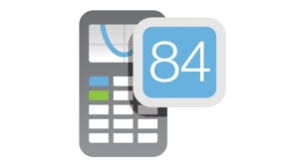
\includegraphics[width=1cm]{TI84Plus-icoon}}}
\newcommand{\grmref}[1]{%
	\reversemarginpar%
	\marginpar{
		\vspace{-0.4cm}%
		\htmladdnormallink{\grmlink}{#1}
	}	
}

% GRM knoppen:
\newcommand{\GRM}[1]{\fbox{\rule[0mm]{0cm}{0.215cm}\textup{\texttt{#1}}}}
\newcommand{\wedgetext}{{\raisebox{0.02cm}{\begin{turn}{90}>\end{turn}}}}
\newcommand{\veetext}{\raisebox{0.2cm}{\begin{turn}{-90}>\end{turn}}}

% voor kolommen met GRM screens:
\newlength{\widthallscreens}
\newlength{\widthscreens}
\newlength{\spaceleftscreen}
\newlength{\spacerightscreen}
\newlength{\spacebetweenscreens}

\newcommand{\setscreens}{
	\setlength{\spaceleftscreen}{2pt}
	\setlength{\spacerightscreen}{2pt}
	\setlength{\spacebetweenscreens}{8pt}
	\addtolength{\linewidth}{-28pt} % 3*8pt tussen vier screens en 2 pt links en 2 pt rechts
	\setlength{\widthallscreens}{\linewidth}
	\setlength{\widthscreens}{0.25\widthallscreens}
	\addtolength{\linewidth}{28pt}
	\newcolumntype{G}{p{\widthscreens}}
	\newcolumntype{s}{p{\spacebetweenscreens}}
	\newcolumntype{L}{p{\spaceleftscreen}}
	\newcolumntype{R}{p{\spacerightscreen}}
	\setlength{\tabcolsep}{0pt}
}

% voor icoon met verwijzing naar Wiskunde Samen gevat² in de marge:
% \newcommand{\wsglink}{\raisebox{0cm}{\includegraphics[width=1cm]{wsglogo}}}
\newcommand{\wsglink}{\raisebox{0cm}{LOGO}}
\newcommand{\htmladdnormallink}[2]{\href{#2}{#1}}
\newcounter{pagnrwsg}
\newcommand{\wsgref}[3]{% 
    % #1 woord dat onderstippeld wordt
    % #2 pagina van Wiskunde Samen gevat² waar je op terecht komt als je op de link klikt  
    % #3 afgedrukt op het logo van Wiskunde Samen gevat² in de marge: één of meerdere paginanummers
    \ifthenelse{\wsg < 1}{#1}{%
        \underdashed{#1}%
        {\setcounter{pagnrwsg}{#2}}%
        {\addtocounter{pagnrwsg}{14}}%
        \reversemarginpar%
        \marginpar{\vspace{-0.6cm}%
           \htmladdnormallink{\wsglink}{https://online.fliphtml5.com/sanky/laea/\#p=\arabic{pagnrwsg}}%
            \raisebox{0.41cm}[0cm][0cm]{%
                \hspace{-1.5cm}\makebox[2cm][c]{\colorbox{white}{\texttt{\footnotesize{#3}}}}%
            }%
        }%
    }%
}

% voor invoegen blanco pagina bij de optie recto-verso:
\def\blancobijrectoverso{
	\ifthenelse{\rectoverso < 1}{\clearpage}{
	\clearpage
	\thispagestyle{empty}
	\mbox{}
	\clearpage
	}
}

% aantal pagina's van het bestand:
\ifthenelse{\rectoverso < 1}{\def\totpag{57}}{\def\totpag{66}}

% documenteigenschappen:
% \usepackage{hyperxmp}
% \hypersetup{
% pdftitle={Open Source Wiskunde Aan zet: Veeltermen}, 
% pdfnumpages={\totpag},
% pdfauthor={Koen De Naeghel},
% pdflang={nl},
% pdfkeywords={wiskunde, open source, wiskunde aan zet, veeltermen, secundair onderwijs, tweede graad, doorstroomfinaliteit},
% pdfsubject={Veeltermen},
% pdfcopyright={\unichar{"24B8} 2024 Koen De Naeghel},
% pdfdate={17 december 2024},
% pdfapart=1,
% pdfstartview=}

% voor het benoemen van titel, auteur en datum:
% \title{Veeltermen}
% \author{Auteur: Koen De Naeghel}
% \date{\today}

\newcommand\BackgroundPic{
    \put(-260,-125){
    \parbox[b][\paperheight]{\paperwidth}{%
    \vfill
    \centering
    
\includegraphics[height=\paperwidth, keepaspectratio]{WaZlogo}%
    \vfill
}}}

% marges:
% \usepackage[paper=a4paper,margin=3.4cm,marginparwidth=2cm]{geometry}
% \usepackage[margin=.5in, includehead, includefoot, hmargin={.8in,.5in}, a4paper]{geometry}
% zes voorkeuren die je meteen zelf kan instellen:
\def\uitbr{1} % waarde 1 als je Uitbreiding in de marge wilt, 0 als je dat niet wilt 
\def\wsg{0} % waarde 1 als je verwijzingen naar Wiskunde Samen gevat² wilt, 0 als je dat niet wilt (onderstippelde woorden in de hoofdtekst en logo met paginanummer en hyperlink naar boekpagina in de marge)
\def\rectoverso{0} % waarde 1 als je het PDF-bestand recto-verso wilt laten afdrukken, 0 als je het recto wilt
\def\voetn{0} % waarde 1 als je de voetnoten wilt, 0 als je dat niet wilt 
\def\grm{0} % waarde 1 als je de schermafdrukken van TI-84 Plus wilt, 0 als je dat niet wilt
\def\grmlogo{0} % waarde 1 als je logo TI-84 Plus in de marge wilt, 0 als je dat niet wilt (met hyperlink naar filmpje) 



% packages algemeen:
\pdfOnly{
% \usepackage[english,dutch]{babel}
}
\usepackage{amsfonts}
\usepackage{amsmath} %  o.a. \eqref en \text, omgeving equation*
\usepackage{amssymb} % o.a. \nmid
\usepackage{amsthm} % o.a. omgeving proof
\usepackage{graphicx} % o.a. figuren
\usepackage{xcolor} % \color
% \usepackage[disable]{todonotes} % \todo 
\usepackage{comment} % omgeving comment
\usepackage{xcolor} % kleuren 
\usepackage[skip=7pt plus1pt, indent=0pt]{parskip} % skip = verticale ruimte tussen twee alinea's, indent = insprong bij nieuwe alinea
\usepackage{multicol} % kolommen
\usepackage{xfrac} % breuken

\usepackage{siunitx} % SI eenheden
\usepackage{eso-pic} % achtergrond voorpagina
\usepackage{tabularx} % kolommen voor rekenmachine
\usepackage{rotating} % voor omgeving turn

% voor figuren met PSTricks:
\usepackage{pstricks} 
\usepackage{pstricks-add}
\usepackage{pst-plot}
\usepackage{pst-node}
\usepackage{pst-coil}
\usepackage{auto-pst-pdf}

% voor figuren met TikZ:
\usepackage{tikz} 
\usepackage{tkz-euclide} 
\usepackage{pgfplots} 
\usetikzlibrary{calc,intersections,through,backgrounds,patterns} 
\pgfplotsset{compat=newest}
\usepgfplotslibrary{fillbetween,colormaps}
\usepackage{import}
\usepackage{tikz-3dplot}

% zelfde parskip in minipage:
\makeatletter
\setlength{\parskip}{\medskipamount}
\newcommand{\@minipagerestore}{\setlength{\parskip}{\medskipamount}}
\makeatother

% voor veranderen van de naam Bibliografie naar Referentielijst:
\pdfOnly{
\addto\captionsdutch{\renewcommand{\bibname}{Referentielijst}}

% voor trefwoordenlijst:
\usepackage{imakeidx}
\makeindex[title=Trefwoordenlijst,program=makeindex,options=-s index.tex,columns=2,intoc=true]
}
% voor nummeren van vergelijkingen:
%WIM%\numberwithin{equation}{chapter} % als je dit desactiveert dan worden vergelijkingen in bijvoorbeeld hoofdstuk 3 genummerd als (1), (2) etc. in plaats van (3.1), (3.2) etc.

% voor hyperlinks en bladwijzers in PDF-bestand:
%WIM%\usepackage[bookmarksopen,bookmarksopenlevel=0,hypertexnames=false,pdfa,bookmarksnumbered]{hyperref} 
%WIM%\usepackage{bookmark} 

% voor hyperlinks: 
\hypersetup{pdfborder={0 0 0}, pdfstartpage=1,linkbordercolor={1 0 0}}%pdfborder={0 0 0} is geen rand rond hyperlinks, pdfborder={1 1 1} wel

% korter commando voor displaystyle, om bijvoorbeeld breuken groter te drukken in doorlopende tekst: 
\newcommand{\D}{\displaystyle}

% (veel)gebruikte verzamelingen:
\newcommand\NN{\mathbb{N}} % verzameling van de natuurlijke getallen
\newcommand\QQ{\mathbb{Q}} % verzameling van de rationale getallen
\newcommand\RR{\mathbb{R}} % verzameling van de re\"ele getallen
\newcommand\ZZ{\mathbb{Z}} % verzameling van de gehele getallen

% (veel)gebruikte operatoren:
\def\co{\operatorname{co}} % coördinaat van een punt
\def\ggd{\operatorname{ggd}} % positieve grootste gemene deler van twee gehele getallen niet beide nul
\def\gr{\operatorname{gr}} % graad van een veelterm

% voor kleur grafieken (donkergroen):
\definecolor{graf}{RGB}{0,100,0} 

% voor lijsten: 
% \usepackage{enumerate}
% \usepackage[shortlabels]{enumitem} 
\setlist{topsep=0em, itemsep=-0.15em}

% voor small bullet:
\newcommand\sbullet[1][.5]{\mathbin{\vcenter{\hbox{\scalebox{#1}{$\bullet$}}}}}

% voor meer verticale ruimte tussen vergelijkingen in align
\addtolength{\jot}{0.1cm}

% voor meervoudige voetnoten:
\usepackage{fnpct}

% voor het onderdrukken van voetnoten als optie:
\usepackage{letltxmacro}
\LetLtxMacro\Oldfootnote\footnote
\newcommand{\EnableFootNotes}{%
  \LetLtxMacro\footnote\Oldfootnote%
}
\newcommand{\DisableFootNotes}{%
  \renewcommand{\footnote}[2][]{\relax}
}

% voor verticale lijn in de marge (uitbreiding):
\usepackage[framemethod=default]{mdframed}
\usepackage{marginnote}
\reversemarginpar
\ifthenelse{\uitbr < 1}{\definecolor{rood}{RGB}{255,255,255}}{\definecolor{rood}{RGB}{254,64,64}} %HEX: #fe4040
\mdfdefinestyle{uitbreiding}{%
    topline=false,
    rightline=false,
    bottomline=false,
    leftline=true,
    linecolor=rood,
    linewidth=5pt,
    rightmargin=0pt,
    skipabove=10pt,% ipv 3
    skipbelow=0pt,
    leftmargin=-25pt,
    innerleftmargin=20pt,
    innerrightmargin=0pt,
    innertopmargin=0pt,
    innerbottommargin=0pt%,
%	needspace=30pt %minimumhoogte vooraleer lijn wordt gesplitst
    }
% \newenvironment{Uitbreiding}{
%     \marginpar{
%         \center
% 		\vspace{0.1cm}
% 		\vspace{7pt}
% 		\rotatebox{90}{\color{rood}\Large \bf Uitbreiding}
% 	}
%     \begin{mdframed}[style=uitbreiding]
%     }{\vspace{-0.05cm}
%     \end{mdframed}
% }

\newenvironment{Uitbreiding}{\begin{xmuitweiding}}{\end{xmuitweiding}}
% omgevingen voor lemma, definitie, voorbeeld etc.:
\newtheoremstyle{mystyle}
    {0em} % Space above
    {0em} % Space below
    {\itshape} % Body font
    {} % Indent amount
    {\bfseries} % Theorem head font
    {.} % Punctuation after theorem head
    {.5em} % Space after theorem head
    {} % Theorem head spec (can be left empty, meaning `normal')
\theoremstyle{mystyle}
%WIM%\newtheorem{lemma}{Lemma}[chapter] % als je [chapter] desactiveert dan Voorbeeld 3 in plaats van Voorbeeld 5.3, als je [chapter] vervangt door [section] dan Voorbeeld 5.2.3 in plaats van Voorbeeld 5.3 
%\theoremstyle{definition} % als je dit activeert dan is wat in de omgeving staat niet cursief gedrukt
\newtheorem{oefening}[lemma]{Oefening}
\newtheorem{definitie}[lemma]{Definitie} 
\newtheorem{voorbeeld}[lemma]{Voorbeeld}
\newtheorem{eigenschap}[lemma]{Eigenschap} 
\newtheorem{stelling}[lemma]{Stelling} 
\newtheorem{gevolg}[lemma]{Gevolg} 
\newtheorem{afspraak}[lemma]{Afspraak} 
\newtheorem{werkwijze}[lemma]{Werkwijze}

% omgeving proof, aangepaste ruimte: 
\makeatletter
\renewenvironment{proof}[1][\proofname]{\par
  \vspace{-\topsep}% remove the space after the theorem
  \pushQED{\qed}%
  \normalfont
  \topsep0pt \partopsep0pt % no space before
  \trivlist
  \item[\hskip\labelsep
        \itshape
    #1\@addpunct{.}]\ignorespaces
}{%
  \popQED\endtrivlist\@endpefalse
  \addvspace{0pt plus 0pt} % no space after
}
\makeatother

% kaderstijlen uit SOHO Wiskunde Plantyn:
\colorlet{steunkleur}{black}
\colorlet{steunkleurlicht}{steunkleur!30!white}
\colorlet{steunkleurkader}{steunkleur!7!white}
\colorlet{steunkleurkaderlicht}{steunkleur!2!white}

\mdfdefinestyle{kaderstijl_vol_licht}
{skipabove=6pt, 
skipbelow=6pt, 
backgroundcolor=steunkleurkader,
linecolor=steunkleurlicht,
linewidth = 0.4pt, 
topline=true,
bottomline=true, 
rightline=true,
innerleftmargin=5pt,
innerrightmargin=5pt,
innertopmargin=5pt,
leftmargin=0cm,
rightmargin=0cm,
innerbottommargin=5pt,
needspace=30pt % minimumhoogte voor splitsen kader
}
\surroundwithmdframed[style=kaderstijl_vol_licht]{definitie}
\surroundwithmdframed[style=kaderstijl_vol_licht]{stelling}
\surroundwithmdframed[style=kaderstijl_vol_licht]{lemma}
\surroundwithmdframed[style=kaderstijl_vol_licht]{eigenschap}
\surroundwithmdframed[style=kaderstijl_vol_licht]{gevolg}

% voor omgevingen voor oefening en antwoord:
\newenvironment{Oefening}{%
    \begin{enumerate}[ 
    series=Oef,
    resume=Oef,
    leftmargin=1.78em,
    label={\bfseries\arabic*.},
    ref=\arabic*
    ]
    \item %
    }{%
    \end{enumerate}
}
\newenvironment{Antwoord}{%
    \begin{enumerate}[%
    series=Antw,
    resume=Antw,
    leftmargin=1.78em,
    label={\bfseries\arabic*.},
    ref=\arabic*
    ]
    \item %
    }{%
    \end{enumerate}
}

% als de omgeving Uitbreiding start met een kaderomgeving (definitie, stelling, eigenschap, lemma of gevolg) dan moet wat extra verticale ruimte voorzien worden, met het commando \uitbreidingstartmetkader:
\def\uitbreidingstartmetkader{\mbox{}\vspace{-0.205cm}}

%WIM % voor schema van de staartdeling:
\usepackage{stackengine}
\setstackgap{S}{5pt}
\stackMath\def\stackalignment{r}
\newcommand{\myRule}[3][white]{\textcolor{#1}{\rule{#2}{#3}}}
\let\ph\phantom % enkel voor tekst
\newcommand{\mph}[1]{% enkel voor math mode
    \mathcolor{white}{#1}%
}
\def\staartmin{\rule{0.25cm}{0.1mm}\myRule{0.3cm}{0.1mm}}
\def\staartphmin{\myRule{0.25cm}{0.1mm}\myRule{0.3cm}{0.1mm}}
\newcommand{\staartstreep}[1]{\rule{\widthof{$#1$}}{0.1mm}}
\newcommand{\staartphstreep}[1]{\myRule{\widthof{$#1$}}{0.1mm}}

% voor kolommen met schema van Horner:
\newcommand{\kolbreed}{1.0cm}
\newcolumntype{H}{>{\centering\arraybackslash$} p{\kolbreed} <{$}}

% voor nieuw commando utikzdashed: onderlijn (zoals underline) maar dan met stippellijn:
\tikzset{
    cheating dash/.code args={on #1 off #2 ends #3}{%
        \csname tikz@addoption\endcsname{%
            \pgfgetpath\currentpath%
            \pgfprocessround{\currentpath}{\currentpath}%
            \csname pgf@decorate@parsesoftpath\endcsname{\currentpath}{\currentpath}%
            \pgfmathparse{max(#1-#3,0)}\let\dashphase=\pgfmathresult%
            \pgfmathparse{\csname pgf@decorate@totalpathlength\endcsname-#1+2*\dashphase}\let\rest=\pgfmathresult%
            \pgfmathparse{#1+#2}\let\onoff=\pgfmathresult%
            \pgfmathparse{max(floor(\rest/\onoff), 1)}\let\nfullonoff=\pgfmathresult%
            \pgfmathparse{max((\rest-\onoff*\nfullonoff)/\nfullonoff+#2, #2)}\let\offexpand=\pgfmathresult%
            \pgfsetdash{{#1}{\offexpand}}{\dashphase pt}}%
    },
    cheating dash per segment/.style args={on #1 off #2 ends #3}{
        /utils/exec=\csname tikz@options\endcsname,%
        decoration={show path construction,
            lineto code={\draw [cheating dash=on #1 off #2 ends #3] (\tikzinputsegmentfirst) -- (\tikzinputsegmentlast);},
            curveto code={\draw [cheating dash=on #1 off #2 ends #3] (\tikzinputsegmentfirst) .. controls (\tikzinputsegmentsupporta) and (\tikzinputsegmentsupportb) .. (\tikzinputsegmentlast);},
            closepath code={\draw [cheating dash=on #1 off #2 ends #3] (\tikzinputsegmentfirst) -- (\tikzinputsegmentlast);}
        },
        decorate,
    },
}
\newcommand{\utikzdash}[1]{%
    \tikz[baseline=(todotted.base)]{
        \node[inner sep=0pt,outer sep=1.5pt] (todotted) {#1};
        \draw[cheating dash per segment=on 2pt off 2pt ends 2pt, line width=0.4pt] (todotted.south west) -- (todotted.south east);
    }%
}%

% voor nieuw commando underdashed: onderlijn met stippellijnen en ook het woord cursief zetten:
\newcommand{\underdashed}[1]{%
    {\em\utikzdash{\!#1\!}}%
}

% voor icoon TI-84 Plus met verwijzing naar filmpje:
\newcommand{\grmlink}{\raisebox{0cm}{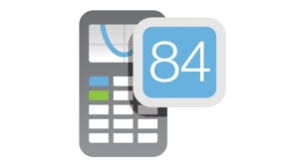
\includegraphics[width=1cm]{TI84Plus-icoon}}}
\newcommand{\grmref}[1]{%
	\ifthenelse{\grmlogo < 1}{}{
		\reversemarginpar%
		\marginpar{
			\vspace{-0.4cm}%
			\htmladdnormallink{\grmlink}{#1}
		}
	}	
}

% GRM knoppen:
\newcommand{\GRM}[1]{\fbox{\rule[0mm]{0cm}{0.215cm}\textup{\texttt{#1}}}}
\newcommand{\wedgetext}{{\raisebox{0.02cm}{\begin{turn}{90}>\end{turn}}}}
\newcommand{\veetext}{\raisebox{0.2cm}{\begin{turn}{-90}>\end{turn}}}

% voor kolommen met GRM screens:
\newlength{\widthallscreens}
\newlength{\widthscreens}
\newlength{\spaceleftscreen}
\newlength{\spacerightscreen}
\newlength{\spacebetweenscreens}

\newcommand{\setscreens}{
	\setlength{\spaceleftscreen}{2pt}
	\setlength{\spacerightscreen}{2pt}
	\setlength{\spacebetweenscreens}{8pt}
	\addtolength{\linewidth}{-28pt} % 3*8pt tussen vier screens en 2 pt links en 2 pt rechts
	\setlength{\widthallscreens}{\linewidth}
	\setlength{\widthscreens}{0.25\widthallscreens}
	\addtolength{\linewidth}{28pt}
	\newcolumntype{G}{p{\widthscreens}}
	\newcolumntype{s}{p{\spacebetweenscreens}}
	\newcolumntype{L}{p{\spaceleftscreen}}
	\newcolumntype{R}{p{\spacerightscreen}}
	\setlength{\tabcolsep}{0pt}
}

% voor icoon met verwijzing naar Wiskunde Samen gevat² in de marge:
\newcommand{\wsglink}{\raisebox{0cm}{\includegraphics[width=1cm]{wsglogo}}}
\newcommand{\htmladdnormallink}[2]{\href{#2}{#1}}
\newcounter{pagnrwsg}
\newcommand{\wsgref}[3]{% 
    % #1 woord dat onderstippeld wordt
    % #2 pagina van Wiskunde Samen gevat² waar je op terecht komt als je op de link klikt  
    % #3 afgedrukt op het logo van Wiskunde Samen gevat² in de marge: één of meerdere paginanummers
    \ifthenelse{\wsg < 1}{#1}{%
        \underdashed{#1}%
        {\setcounter{pagnrwsg}{#2}}%
        {\addtocounter{pagnrwsg}{14}}%
        \reversemarginpar%
        \marginpar{\vspace{-0.6cm}%
           \htmladdnormallink{\wsglink}{https://online.fliphtml5.com/sanky/laea/\#p=\arabic{pagnrwsg}}%
            \raisebox{0.41cm}[0cm][0cm]{%
                \hspace{-1.5cm}\makebox[2cm][c]{\colorbox{white}{\texttt{\footnotesize{#3}}}}%
            }%
        }%
    }%
}

% voor invoegen blanco pagina bij de optie recto-verso:
\def\blancobijrectoverso{
	\ifthenelse{\rectoverso < 1}{\clearpage}{
	\clearpage
	\thispagestyle{empty}
	\mbox{}
	\clearpage
	}
}

% aantal pagina's van het bestand:
\ifthenelse{\rectoverso < 1}{\def\totpag{57}}{\def\totpag{66}}

% documenteigenschappen:
% \usepackage{hyperxmp}
% \hypersetup{
% pdftitle={Open Source Wiskunde Aan zet: Veeltermen}, 
% pdfnumpages={\totpag},
% pdfauthor={Koen De Naeghel},
% pdflang={nl},
% pdfkeywords={wiskunde, open source, wiskunde aan zet, veeltermen, secundair onderwijs, tweede graad, doorstroomfinaliteit},
% pdfsubject={Veeltermen},
% pdfcopyright={\unichar{"24B8} 2024 Koen De Naeghel},
% pdfdate={17 december 2024},
% pdfapart=1,
% pdfstartview=}

% voor het benoemen van titel, auteur en datum:
% \title{Veeltermen}
% \author{Auteur: Koen De Naeghel}
% \date{\today}

\newcommand\BackgroundPic{
    \put(-260,-125){
    \parbox[b][\paperheight]{\paperwidth}{%
    \vfill
    \centering
    
\includegraphics[height=\paperwidth, keepaspectratio]{WaZlogo}%
    \vfill
}}}


\newcommand{\chapter}{\section}

% voor figuren met PSTricks:
\usepackage{pstricks} 
\usepackage{pstricks-add}
\usepackage{pst-plot}
\usepackage{pst-node}
\usepackage{pst-coil}
%\usepackage{auto-pst-pdf}


\addPrintStyle{.}

\begin{document}

% \renewcommand{\floatpagefraction}{0.8}
% \renewcommand{\textfraction}{0.1}
% \renewcommand{\topfraction}{0.9}
% \renewcommand{\bottomfraction}{0.9}


% \frontmatter
% \pdfbookmark[section]{Titelpagina}{Tit}
% \makeatletter
% \begin{titlepage}
% \AddToShipoutPicture*{\BackgroundPic}
% \begin{center}
% {\Huge \sl Open Source}  \\[0.5cm]
% {\Huge \sl Wiskunde Aan\,zet} \\[1.2cm]
% {\huge \bfseries  \@title} \\[1.2cm]
% {\Large  \@author}
% \end{center}
% \end{titlepage}
% \makeatother
% \thispagestyle{empty}

% % bij optie recto-verso een pagina met specificaties en extra titelblad invoegen %%%
% \ifthenelse{\rectoverso < 1}{%%% \clearpage}{
% 	%%% \clearpage
% 	\pagestyle{empty}
% 	\mbox{}
% 	\addtocounter{page}{-1}
% 	%%% \clearpage
% 	\begin{center}
% 	{\Huge \sl Open Source}  \\[0.5cm]
% 	{\Huge \sl Wiskunde Aan\,zet} \\[1.2cm]
% 	{\huge \bfseries  Veeltermen} \\[1.2cm]
% 	{\Large  Auteur: Koen De Naeghel}
% 	\end{center}
% 	%%% \clearpage
% 	\mbox{}
% 	\vfill{
% 		\xmemph{Gepubliceerd door:} 
% 		Online uitgever Lulu.com 

% 		\xmemph{Omslagfoto:} 
% 		\url{https://www.shutterstock.com}, ID: 110461682

% 		\xmemph{Tekstzetsysteem:} \LaTeX{}

% 		\xmemph{Royalty percentage:} $0\%$ 

% 		\copyright\, 2024 Koen De Naeghel

% 		\xmemph{Licentie:} Creative Commons Naamsvermelding-NietCommercieel-GelijkDelen 4.0 \\
% 		{\color{white}\xmemph{Licentie:}} Internationaal (CC BY-NC-SA) 

% 		ISBN 978-1-326-76411-1 

% 		Eerste druk, december 2024
% 	}
% }
% %%%%%%%%%%%%%%%%%%%%%%%%%%%%%%%%%%%%%%%%%%%%%%%%%%%%%%%%%%%%%%%%%%%%%%%%%%%%%%%%%%%%

% \chapter{Licentievoorwaarden} 
% \label{rechten}
% \pagestyle{plain}

% Dit werk is gelicenseerd onder CC BY-NC-SA 4.0, voluit: 
% \begin{center}
% Creative Commons Naamsvermelding-NietCommercieel-GelijkDelen 4.0 Internationaal. 
% \end{center}
% Op deze pagina worden enkele van de belangrijkste kenmerken en voorwaarden van de volledige licentie belicht. Die vereenvoudigde versie (akte) is ontleend aan 
% \begin{center}
% \url{https://creativecommons.org/licenses/by-nc-sa/4.0/legalcode.nl}. 
% \end{center}
% We raden aan om alle voorwaarden van de volledige licentie te bestuderen voordat je het gelicenseerde materiaal gebruikt. De volledige, juridische tekst vind je op
% \begin{center}
% \url{http://creativecommons.org/licenses/by-nc-sa/4.0/nl/legalcode}. 
% \end{center}







% \par

% {\bf Je bent vrij om:}
% \begin{itemize}
% \item[]
% {\bf Delen} - het materiaal te kopi\"eren, te verspreiden en door te geven via elk medium of bestandsformaat.
% \item[]
% {\bf Bewerken} - te remixen, te veranderen en afgeleide werken te maken.
% \item[]
% De licentiegever kan deze toestemming niet intrekken zolang aan de licentievoorwaarden voldaan wordt.
% \end{itemize}

% \par

% {\bf Onder de volgende voorwaarden:} 
% \begin{itemize}
% \item[]
% {\bf Naamsvermelding} - De gebruiker dient de maker van het werk te vermelden, een link naar de licentie te plaatsen en aan te geven of het werk veranderd is. Je mag dat op redelijke wijze doen, maar niet zodanig dat de indruk gewekt wordt dat de licentiegever instemt met je werk of je gebruik van het werk.
% \item[]
% {\bf Niet-commercieel} - Je mag het werk niet gebruiken voor commerci\"ele doeleinden.
% \item[]
% {\bf Gelijk delen} - Als je het werk hebt geremixt, veranderd, of op het werk hebt voortgebouwd, moet je het veranderde materiaal verspreiden onder dezelfde licentie als het originele werk.
% \item[]
% {\bf Geen aanvullende restricties} — Je mag geen juridische voorwaarden of technologische voorzieningen toepassen die anderen er juridisch in beperken om iets te doen wat de licentie toestaat.
% \end{itemize}

% \par

% {\bf Let op:} 

% Voor elementen van het materiaal die zich in het publieke domein bevinden, en voor vormen van gebruik die worden toegestaan via een uitzondering of beperking in de Auteurswet, hoef je je niet aan de voorwaarden van de licentie te houden. 

% Er worden geen garanties afgegeven. Het is mogelijk dat de licentie je niet alle gebruiksvrijheden geeft die nodig zijn voor het beoogde gebruik. Bijvoorbeeld, andere rechten zoals publiciteits-, privacy- en morele rechten kunnen het gebruik van een werk beperken.

% %%% \blancobijrectoverso


\chapter{Voorwoord}

Dit boekdeel is bestemd voor leerlingen van de tweede graad doorstroomfinaliteit van het secundair onderwijs met minstens vijf wekelijkse lestijden wiskunde. Het verwezenlijkt twee differenti\"ele doelen, opgelegd door de Vlaamse Overheid voor de richtingen economische wetenschappen, Grieks-Latijn, Latijn, natuurwetenschappen, technologische wetenschappen:
\begin{center}
\begin{minipage}{13cm}\itshape
\begin{enumerate}
\item[DD1]
De leerlingen bewijzen wiskundige uitspraken. \\
$\sbullet[.75]$ Bewijstechnieken: rechtstreeks bewijs, bewijs uit het ongerijmde
\item[DD6]
De leerlingen analyseren deelbaarheid bij veeltermen met re\"ele co\"efficiënten in \'e\'en variabele. \\
$\sbullet[.75]$ Euclidische deling, reststelling
\end{enumerate}
\end{minipage}
\end{center}
Er werden enkele ingrepen gedaan om de haalbaarheid van de leerstof in 14 lesuren te garanderen. Paragrafen en oefeningen waarbij \textit{Uitbreiding} in de marge staat, hoeven niet behandeld te worden. Van eigenschappen die overtuigend geduid kunnen worden aan de hand van een concreet voorbeeld, kan het formele bewijs achterwege gelaten worden. Bij een krappere timing komen de basisbegrippen dus niet in het gedrang.

De strakke vorm van deze cursus is voor leerlingen mogelijk ongewoon, maar een goede voorbereiding op cursussen in de derde graad doorstroomfinaliteit en in het hoger onderwijs. In deze tekst duiden onderlijnde woorden op een eerste omschrijving van dat begrip. De trefwoordenlijst achteraan laat toe dergelijke omschrijvingen snel terug te vinden. Na elk hoofdstuk zijn de oefeningen verdeeld in drie reeksen: eenvoudig, gemiddeld en verdiepend of verbredend. Achteraan het boek staan de eindantwoorden van de oefeningen.

De inhoud van dit werk is afgeleid uit onderdelen van de invulcursussen \xmemph{Wiskunde Aan\,zet} en \xmemph{Wiskunde In\,zicht}, zie \cite{waz,wiz} achteraan in de referentielijst. Enkele voorbeelden en oefeningen komen uit \cite{TAOPS-intalg} en \cite{Dhont}. Er werden ook vragen uit voorbije toelatingsexamens arts opgenomen \cite{toelatingsexamens}. Voor de vormgeving van dit boek en enkele passages in dit voorwoord werd beroep gedaan op de cursus \xmemph{Algebra\"ische structuur: de vectorruimte $\RR,\RR^n,+$} van Wiskundeplan \cite{Wiskundeplan:cursus}. De kaderstijl voor definities en eigenschappen werd ontleend aan \cite{Kuijpers}. 

Deze publicatie is digitaal beschikbaar op de website 
\begin{center}
\url{https://www.koendenaeghel.be/opensource.htm}
\end{center}
waar ook een link staat naar de broncode in Overleaf. Wie dat wenst, kan met het tekstzetprogramma \LaTeX{} een afgeleid werk kan maken, mits het respecteren van de voorwaarden zoals vermeld op pagina \pageref{rechten}.
Daarbij kan de gebruiker zelf enkele voorkeuren instellen voor het aanmaken van een PDF-bestand, zoals het (des)activeren van de indicatie \textit{Uitbreiding} in de marge en de verwijzingen naar het pocketboekje \xmemph{Wiskunde Samen\,gevat\,${}^{2}$}, zie \cite{wsg}. 

Dit werk heeft niet de pretentie origineel, foutloos, volledig of afgewerkt te zijn, of erger nog de intentie te hebben van: \xmemph{zo moet het}. De auteur wil enkel laten zien: \xmemph{misschien kan het zo ook}, en hoopt met deze vrije publicatie leerlingen en leerkrachten te inspireren en bij te dragen aan een haalbaar kwalitatief wiskundeonderwijs.

\vfill{
\begin{flushright}
Koen De Naeghel \\
Brugge, december 2024
\end{flushright}
}

%%% \blancobijrectoverso
\renewcommand{\contentsname}{\huge{Inhoud}} 
% \pdfbookmark[chapter]{Inhoud}{Inh}
% \tableofcontents

%%% \blancobijrectoverso
% aantal pagina's in frontmatter bijhouden, nodig voor trefwoordenlijst achteraan:
\newcounter{totaalaantalvoorbladen}
\setcounter{totaalaantalvoorbladen}{\value{page}}
\ifthenelse{\rectoverso < 1}{}{\addtocounter{totaalaantalvoorbladen}{1}}

% optie onderdrukken van de voetnoten:
\ifthenelse{\voetn < 1}{\DisableFootNotes}{}

% \mainmatter




\chapter{Basisbegrippen}

In de voorbije jaren heb je leren rekenen met lettervormen, waaronder het optellen, ver\-menigvuldigen en vereenvoudigen van eentermen, tweetermen en drietermen. Dat zullen we in dit hoofdstuk uitbreiden tot viertermen, vijftermen enzovoort. Algemeen spreken we dan van \xmemph{veeltermen}.

\section{Eentermen}

De bewerkingen
\[
2\cdot 3^5, \qquad 2\cdot 8^5, \qquad 2\cdot (-1)^5, \qquad 2\cdot\left(\frac{19}{3}\right)^5, \qquad 2\cdot\left(\sqrt{3}\right)^5 \qquad \text{ en } \qquad 2 \cdot \pi^5
\]
hebben iets gemeen: ze zijn allemaal van de vorm $2\cdot \square^5$ waarbij $\square$ een \wsgref{re\"eel getal}{27}{27} voorstelt. Het is gebruikelijk om in plaats van het symbool $\square$ een Latijnse letter zoals $x$ te schrijven, die we dan een \xmemph{variabele} noemen. De bewerkingen hierboven zijn dan telkens van de vorm $2 \cdot x^5$ en die uitdrukking noemen we een \xmemph{eenterm in $x$}. Daarbij wordt het symbool $\cdot$ voor de vermenigvuldiging meestal weggelaten. 

Doorgaans noteren we een eenterm met een Latijnse hoofdletter zoals $A$ of $B$. Om te beklemtonen dat de variabele van de eenterm gelijk is aan $x$, noteren we dan ook $A(x)$ of $B(x)$. Wat tussen de haakjes staat, noemen we dan het \xmemph{argument}, wat in dit geval gewoon gelijk is aan de variabele $x$. De eenterm van hierboven kan nu geschreven worden als $A(x) = 2x^5$ en veralgemenen leidt tot de volgende definitie.

\begin{definition}
Een \underline{(re\"ele) eenterm in (de variabele) $x$}\index{eenterm} is een uitdrukking $A(x) = ax^n$ waarbij $a \in \RR$ en $n \in \NN$. 
\end{definition}

Spreken we in het vervolg van \xmemph{een eenterm} $A(x) = ax^n$ of $B(x) = bx^m$ dan nemen we steeds aan dat $n,m\in \NN$ en $a,b\in \RR$.

\begin{example}
De volgende uitdrukkingen zijn eentermen in $x$:
\[
A(x) = 2x^5, \quad B(x) = -\frac{3}{7}\,x^1, \quad C(x) = 541x^0 \quad \text{ en } \quad D(x) = 0x^{2024}.
\]
Ook $A(t) = 2t^5$ is een eenterm, maar dan in de variabele $t$. De volgende uitdrukkingen zijn geen eentermen in $x$:
\[
2x^5+3x, \quad \frac{1}{x}, \quad 3x^{-5}, \quad \sqrt{x} \quad \text{en} \quad \left|x\right|.
\] 
\end{example}

De uitdrukking $ax^n$ van een eenterm wordt opgevat als de \xmemph{vermenigvuldiging} van een re\"eel getal $a$ met $x^n$. Om die vermenigvuldiging te benadrukken, noteren we $ax^n$ soms ook als $a \cdot x^n$. Verder vatten we de uitdrukking $x^n$ op als \wsgref{macht}{45}{45} met als grondtal de variabele $x$ en als exponent $n$. Bij afspraak maken we dan ook gebruik van de volgende schrijfwijzen:
\[
1\cdot x^n = x^n, \qquad
0\cdot x^n = 0, \qquad  
x^0 = 1, \qquad 
a\cdot x^0 = a \qquad \text{ en } \qquad 
a\cdot x^1 = a \cdot x = ax.
\]

Als $ax^n$ een eenterm is, dan noemen we het getal $a$ de \underline{co\"effici\"ent}\index{co\"effici\"ent}\index{eenterm!co\"effici\"ent} van de eenterm.

\begin{example}
We vereenvoudigen de onderstaande eentermen, geven telkens de co\"eefici\"ent en vermelden ook of de eenterm al dan niet behoort tot de verzameling van de re\"ele getallen.
\begin{enumerate}

\item
$A(x) = \sqrt{2}\cdot x \cdot x \cdot x = \sqrt{2}\cdot x^3$ met co\"effici\"ent $\sqrt{2}$, en $A(x) \not\in \RR$
\item
$B(x) = 541x^0 = 541$ met co\"effici\"ent $541$, en $B(x) \in \RR$ 
\item
$\D C(x) = -\frac{4}{7}\,x^1 = -\frac{4}{7}\,x$ met co\"effici\"ent $\D -\frac{4}{7}$, en $C(x) \not\in \RR$
\item
$D(x) = 0 x^{2024} = 0$ met co\"effici\"ent $0$, en $D(x) \in \RR$ 
\end{enumerate}
\end{example}

Als $ax^n$ een eenterm is waarbij $a \neq 0$, dan noemen we $n$ de \underline{graad}\index{graad}\index{eenterm!graad} van de eenterm. Schrijven we de eenterm als $A(x)$, dan noteren we de graad als $\gr A(x)$. De graad van de eenterm $0\cdot x^n = 0$ wordt in het secundair onderwijs niet gedefini\"eerd.

\medskip

\begin{Uitbreiding}
In hogere wiskunde stelt men $\gr 0 = - \infty$ omdat op deze manier rekenregels in verband met de graad van een eenterm geldig blijven, bijvoorbeeld 
\xmemph{de graad van het product van twee re\"ele eentermen is gelijk aan de som van de graden van die eentermen}. Daarvoor verwijzen we naar Oefening \ref{oefgraadnulveelterm} op het einde van dit hoofdstuk.
\end{Uitbreiding}

\begin{example}
Beschouw de volgende eentermen.
\[
A(x) = -7x^3, \,\,\, B(x) = -\frac{17}{89}\,x^5\cdot x^3, \,\,\, C(x) = 1, \,\,\, D(x) = \sqrt{5}\,x, \,\,\, P(x) = 0 x^4, \,\,\,  Q(x) = 0 x^7.
\]
De graad van de eenterm $A(x)$ is gelijk aan $3$, in symbolen: $\gr A(x) = 3$. Herschrijven we de andere eentermen als
\[
B(x) = -\frac{17}{89}\,x^8, \qquad C(x) = 1\cdot x^0, \qquad D(x) = \sqrt{5}\,x^1, \qquad P(x) = 0 = Q(x)
\]
dan lezen we hieruit af dat 
\[
\gr B(x) = 8, \qquad \gr C(x) = 0, \qquad \gr D(x) = 1. 
\]
Omdat $P(x) = 0$ bestaat de graad van de eenterm $P(x)$ niet. We schrijven dan: $\gr P(x) = /$. Idem is $\gr Q(x) = /$.
\end{example}

Twee eentermen in $x$ zijn \underline{gelijksoortig}\index{gelijksoortig} als ze ofwel dezelfde graad hebben, ofwel beide gelijk zijn aan nul.

\begin{example}
Gegeven zijn de eentermen
\[
A(x) = -\frac{1}{3}\,x^9, \quad B(x) = 5\,x^9, \quad C(x) = 0x^9, \quad D(x) = 2^9, \quad P(x) = \pi \quad \text{ en } \quad Q(x) = 0 x^7.
\]
Dan zijn $A(x)$ en $B(x)$ gelijksoortig. Omdat $C(x) = 0 = Q(x)$ zijn ook $C(x)$ en $Q(x)$ gelijksoortig. Ten slotte is $D(x) = 2^9 \cdot x^0$ en $P(x) = \pi \cdot x^0$ zodat de eentermen $D(x)$ en $P(x)$ gelijksoortig zijn.  
\end{example}

Twee eentermen in $x$ zijn \underline{gelijk}\index{eenterm!gelijk} als ze ofwel dezelfde graad en dezelfde co\"effici\"ent hebben, ofwel beide gelijk zijn aan nul.

\begin{example}
We hebben dat $0x^{2024} = 0x^{2025}$. En als je weet dat $\sqrt{2}\,x^n = bx^{35}$ dan is $n = 35$ en $b = \sqrt{2}$.
\end{example}


%%% \clearpage

Vervangen we in een eenterm $A(x)$ de variabele $x$ door een re\"eel getal $r$, dan verkrijgen we de \underline{getalwaarde}\index{eenterm!getalwaarde} van $A(x)$ in $x = r$. Die getalwaarde noteren we met $A(r)$. Samengevat: als $A(x) = ax^n$ dan is $A(r) = ar^n$. Met behulp van het symbool $\Rightarrow$ voor \wsgref{implicatie}{2}{2} wordt dit in symbolen:
\[
A(x) = ax^n \quad \Rightarrow \quad A(r) = a r^n.
\]
Hierbij is $a,r \in \RR$ en $n \in \NN$, waarbij we het geval $r = n = 0$ uitsluiten: aan de uitdrukking $0^0$ geven we geen betekenis.

\begin{example}
Als $A(x) = 5x^3$ dan is de getalwaarde van $A(x)$ in $x = -2$ gelijk aan 
\[
A(-2) = 5 \cdot (-2)^3 = 5 \cdot (-8) = - 5 \cdot 8 = -40.
\]
\end{example}

De som of het verschil van twee gelijksoortige eentermen in $x$ is opnieuw een eenterm in $x$, met als rekenregels:
\[
ax^n + bx^n = (a+b)x^n \quad \text{ en } \quad ax^n - bx^n = (a-b)x^n
\]
of kortweg: $ax^n \pm bx^n = (a\pm b)x^n$. Ook het product van twee eentermen in $x$ is opnieuw een eenterm in $x$, waarbij:
\[
ax^n \cdot bx^m = abx^{n+m}.
\]
Na het toepassen van die rekenregels kan een som $a+b$, een verschil $a-b$ of een product $ab$ soms verder uitgewerkt en nadien vereenvoudigd worden. Zo moet je vlot kunnen rekenen met \wsgref{breuken}{37}{37-39}.

\begin{example}
Als $\D A(x) = \frac{3}{4}\,x^5$ en $\D B(x) = -\frac{7}{6}\,x^5$ dan is 
\begin{align*}
A(x) + B(x) & = \frac{3}{4}\,x^5 + \left(-\frac{7}{6}\,x^5\right) 
= \frac{3}{4}\,x^5 - \frac{7}{6}\,x^5
= \left(\frac{3}{4} - \frac{7}{6}\right)x^5 
= \frac{3 \cdot 3 - 7 \cdot 2}{12}\,x^5 
= -\frac{5}{12}\,x^5, \\
A(x) \cdot B(x) & = \frac{3}{4}\,x^5 \cdot \left(-\frac{7}{6}\,x^5\right) = - \frac{3 \cdot 7}{4 \cdot 6}\,x^{5+5} = -\frac{1\cdot 7}{4 \cdot 2}\, x^{10} = -\frac{7}{8}\,x^{10}. 
\end{align*}
\end{example}


\section{Veeltermen}

Als $ax^n$ en $bx^m$ eentermen zijn, dan kunnen we de uitdrukking $ax^n + bx^m$ bekijken, die we opvatten als de \xmemph{som} van die twee eentermen. Het resultaat noemen we een \xmemph{tweeterm}. Analoog kunnen we spreken over een \xmemph{drieterm}, een \xmemph{vierterm} enzovoort. Algemeen spreken we dan van een \xmemph{veelterm}.

\begin{definition}[in woorden]
Een \underline{(re\"ele) veelterm in (de variabele) $x$}\index{veelterm} is een eindige som van eentermen in $x$.
\end{definition}

\begin{example}
De volgende uitdrukkingen zijn veeltermen in $x$:
\[
3x^2, \qquad \sqrt{5} - 8x, \qquad -1 + 3x -2x^2 \qquad \text{ en } \qquad -\frac{4}{3}x^5 - 2x^3 + \pi^2\,x + 5. 
\]
\end{example}

We willen nu ook een willekeurige veelterm in symbolen kunnen schrijven. Als de graad van de eentermen die voorkomen niet te hoog is, kan dat als volgt:
\begin{align*} 
\left\{
\begin{aligned}
& a && \text{ waarbij } a \in \RR  \\
& a + bx && \text{ waarbij } a,b \in \RR  \\
& a + bx + cx^2 && \text{ waarbij } a,b,c \in \RR  \\
& a + bx + cx^2 + dx^3 && \text{ waarbij } a,b,c,d \in \RR \\
& \text{etc.} && 
\end{aligned}
\right.
\end{align*}
Van zodra er een eenterm van graad $26$ voorkomt, hebben we onvoldoende letters in het Latijns alfabet. Dat probleem kunnen we omzeilen door gebruik te maken van een \xmemph{onderindex}\:: in plaats van $a,b,c$ etc. schrijven we $a_0, a_1, a_2$ etc. Op die manier kunnen we een willekeurige veelterm in symbolen uitdrukken.

\begin{definition}[in symbolen]
Een \underline{(re\"ele) veelterm in (de variabele) $x$}\index{veelterm} is een uitdrukking van de vorm $A(x) = a_0 + a_1x + a_2x^2 + \dots + a_n x^n$ waarbij $n \in \NN$ en $a_0,a_1,a_2,\ldots,a_n \in \RR$.
\end{definition}

Spreken we in het vervolg van \xmemph{een veelterm} $a_0 + a_1x + a_2x^2 + \dots + a_n x^n$ of $b_0 + b_1x + \dots + b_m x^m$ dan nemen we steeds aan dat $n,m\in \NN$ en $a_0, \ldots, a_n\in \RR$ en $b_0, \ldots, b_m\in \RR$.

\begin{example}
Kiezen we in de bovenstaande definitie $n = 4$ en $a_0 = -5$, $a_1 = 7$, $a_2 = -3$, $a_3 = 0$ en $a_4 = 0$ dan verkrijgen we de veelterm
\begin{align*}
A(x) 
& = a_0 + a_1x + a_2x^2 + \dots + a_n x^n \\
& = a_0 + a_1x + a_2x^2 + a_3 x^3 + a_4 x^4 \\ 
& = -5 + 7x - 3x^2 + 0x^3 + 0x^4 \\
& = -5 + 7x - 3x^2.
\end{align*}
We konden dus even goed $n = 2$ en $a_0 = -5$, $a_1 = 7$ en $a_2 = -3$ gekozen hebben. 
\end{example}

Dankzij de afspraak $x^0 = 1$ kunnen we een veelterm herschrijven met het \wsgref{sommatieteken}{54}{54}:
\[
A(x) = a_0 + a_1x + a_2x^2 + \dots + a_n x^n = \sum_{i=0}^n a_i x^i.
\]

\begin{example}
Beschouw de veeltermen
\[
A(x) = \sum_{i=0}^3 (2i+1) x^i \qquad \text{ en } \qquad P(t) = \sum_{i=1}^5 \frac{1}{i^2} \, t^i.
\] 
Dan kunnen we die veeltermen uitschrijven als
\begin{align*}
A(x)  = (2\cdot0+1)x^0 + (2\cdot1+1)x^1 + (2\cdot2+1)x^2 + (2\cdot3+1)x^3 = 1 + 3x + 5x^2 + 7x^3
\end{align*}
en
\begin{align*}
P(x) 
& = \frac{1}{1^2} \, t^1 + \frac{1}{2^2} \, t^2 + \frac{1}{3^2} \, t^3 + \frac{1}{4^2} \, t^4 + \frac{1}{5^2} \, t^5 \\
& = t + \frac{1}{4}\,t^2 + \frac{1}{9}\,t^3 + \frac{1}{16}\,t^4 + \frac{1}{5}\,t^5.
\end{align*}
\end{example}

Als $a_0 + a_1x + a_2x^2 + \dots + a_n x^n$ een veelterm is, dan noemen we de getallen $a_0, a_1, a_2, \ldots, a_n$ de \underline{co\"effici\"enten}\index{co\"effici\"ent}\index{veelterm!co\"effici\"enten} van de veelterm. De (een)termen $a_0, a_1x, a_2x^2, \ldots , a_nx^n$ noemen we de \underline{(een)termen} van de veelterm. De term $a_0$ wordt de \underline{constante term}\index{constante term}\index{veelterm!constante term} van de veelterm genoemd.

\begin{example}
De constante term van de veelterm $A(x) = -5 + 7x - 3x^2$ is gelijk aan $-5$.  
\end{example}

Als $a_0 + a_1x + a_2x^2 + \dots + a_n x^n$ een veelterm is waarbij $a_n \neq 0$, dan noemen we $n$ de \underline{graad}\index{graad}\index{veelterm!graad} van de veelterm. Schrijven we de veelterm als $A(x)$, dan noteren we de graad als $\gr A(x)$. In dat geval is $a_nx^n$ de \underline{hoogstegraadsterm}\index{hoogstegraadsterm}\index{veelterm!hoogstegraadsterm} en $a_n$ de \underline{hoogstegraadsco\"effici\"ent}\index{hoogstegraadsco\"effici\"ent}\index{veelterm!hoogstegraadsco\"effici\"ent} van de veelterm. De graad van de veelterm $0 + 0\cdot x + 0 \cdot x^2 + \dots + 0\cdot x^n = 0$ wordt in het secundair onderwijs niet gedefini\"eerd.

Veeltermen van graad nul, \'e\'en, twee of drie wordt respectievelijk \underline{constante}, \underline{lineaire}, \linebreak \underline{kwadratische} en \underline{kubische veeltermen} genoemd. Ook veelterm $0 + 0\cdot x + 0 \cdot x^2 + \dots + 0\cdot x^n = 0$ wordt een constante veelterm genoemd.

\begin{example}
We vereenvoudigen onderstaande veeltermen, en geven telkens de graad, de hoogstegraadsco\"effici\"ent en constante term.
\begin{enumerate}

\item
$A(x) = 1-4x+5x^3-7x^3 = 1 - 4x - 2x^3$ heeft graad $3$, hoogstegraadsco\"effici\"ent $-2$ en constante term $1$.
\item
$B(x) = 0x^2 + 3x = 3x$ heeft graad $1$, hoogstegraadsco\"effici\"ent $3$ en constante term $0$.
\item
$C(x) = \sqrt{7}-\sqrt{28} = \sqrt{7}-2\sqrt{7} = -\sqrt{7}$ heeft graad $0$, hoogstegraadsco\"effici\"ent $-\sqrt{7}$ en constante term $-\sqrt{7}$.
\end{enumerate}
\end{example}

De \wsgref{verzameling}{15}{15} van alle veeltermen in $x$ wordt genoteerd met $\RR[x]$. In symbolen:
\[
\RR[x] = \{a_0 + a_1 x + a_2 x^2 + \dots + a_n x^n \mid \text{$n \in \NN$ en $a_0,a_1,a_2,\ldots,a_n \in \RR$} \}.
\]
Wegens een eerdere afspraak is $a = a\cdot x^0$, zodat elk re\"eel getal $a$ kan geschreven worden als een veelterm. De verzameling van de re\"ele getallen is dus een \wsgref{deelverzameling}{16}{16}
van de verzameling van alle veeltermen, in symbolen: $\RR \subseteq \RR[x]$. 

\begin{example} We hebben dat $1-4x+2x^3 \in \RR[x]$, $x^5-\sqrt{2} \in \RR[x]$ en $\D -\frac{13}{7} \in \RR[x]$.   
\end{example}

Twee veeltermen in $x$ zijn \underline{gelijk} als ze ofwel dezelfde graad en dezelfde co\"effici\"enten hebben, ofwel beide gelijk zijn aan nul. 

Soms komen er in wiskundige uitdrukkingen symbolen zoals $a$, $b$, $p$, $q$ etc. voor die getallen voorstellen. Pas als die symbolen een waarde toegekend krijgen, wordt de uitdrukking volledig vastgelegd. Zo'n symbool noemen we dan een \xmemph{parameter}.\index{parameter} 

\begin{example}
Beschouw $A(x) = ax^5 - 4x^2 + bx + 2$ en $B(x) = 7x^m + 2ax - c^2x^2 - d$ waarbij $a,b,c,d \in \RR$ en $m \in \NN$. We bepalen de waarde(n) van de parameters $a,b,c,d$ en $m$ waarvoor de veelterm $A(x)$ gelijk is aan de veelterm $B(x)$. We hebben: 
\begin{align*}
A(x) = B(x) \quad 
& \Leftrightarrow \quad ax^5 - 4x^2 + bx + 2 = 7x^m + 2ax - c^2x^2 - d \\
& \Leftrightarrow \quad 5 = m \,\,\text{ en }\,\, a = 7 \,\,\text{ en }\,\, -4 = -c^2 \,\,\text{ en }\,\, b = 2a \,\,\text{ en }\,\, 2 = -d \\
& \Leftrightarrow \quad m=5 \,\,\text{ en }\,\, a = 7 \,\,\text{ en }\,\, c^2 = 4 \,\,\text{ en }\,\, b = 14 \text{ en } d = -2 \\
& \Leftrightarrow \quad 
\left\{
\begin{aligned}
& m=5 \,\,\text{ en }\,\, a = 7 \,\,\text{ en }\,\, c = 2 \,\,\text{ en }\,\, b = 14 \text{ en } d = -2 \\
& \text{of} \\
& m=5 \,\,\text{ en }\,\, a = 7 \,\,\text{ en }\,\, c = -2 \,\,\text{ en }\,\, b = 14 \text{ en } d = -2.
\end{aligned}
\right.
\end{align*}
\end{example}

Vervangen we in een veelterm $A(x)$ de variabele $x$ door een re\"eel getal $r$, dan verkrijgen we de \underline{getalwaarde}\index{veelterm!getalwaarde} van $A(x)$ in $x = r$. Die getalwaarde noteren we met $A(r)$. In symbolen:
\[
A(x) = a_0 + a_1x + a_2x^2 + \dots + a_n x^n \quad 
\Rightarrow
\quad A(r) = a_0 + a_1 r + a_2r^2 + \dots + a_n r^n
\]
met $n \in \NN$ en $r, a_0, a_1, \ldots, a_n \in \RR$, waarbij we ook hier het geval $n = r = 0$ uitsluiten. % voor ons heeft $0^0$ geen betekenis.

\begin{example}
Als $A(x) = 2x^3+3x-5$ dan is de getalwaarde van $A(x)$ in $x = 10$ gelijk aan $A(10) = 2\cdot 10^3 + 3 \cdot 10 - 5 = 2025$.
\end{example}

Is de getalwaarde van een veelterm in een re\"eel getal $r$ gelijk aan nul, dan noemen we $r$ een \underline{nulwaarde}\index{veelterm!nulwaarde} \index{nulwaarde} van die veelterm. De uitspraak \xmemph{$r$ is een nulwaarde van $A(x)$} is dus gelijkwaardig met de uitspraak \xmemph{$A(r) = 0$}. Met behulp van het symbool $\Leftrightarrow$ voor \wsgref{equivalentie}{2}{2} wordt dit in symbolen:
\[
r \text{ is een nulwaarde van } A(x) \quad \Leftrightarrow \quad A(r) = 0.
\]
Hierbij is $r \in \RR$ en $A(x)$ een veelterm in $x$. In de literatuur wordt een nulwaarde soms ook een \underline{nulpunt}\index{nulpunt} genoemd. Onze voorkeur gaat uit naar de volgende afspraak: een nulpunt is een punt (dus een meetkundig object), een nulwaarde is een waarde (dus een getal).

Bepalen van de waarde(n) van parameters kan leiden tot een \wsgref{stelsel}{115}{115-119}. 
In het derde jaar heb je geleerd hoe je een stelsel van twee vergelijkingen in twee onbekenden kan oplossen. Die technieken moet je nog steeds kunnen toepassen. 

\begin{example}
We bepalen de waarde(n) van de parameters $a$ en $b$ waarvoor
\[
a(x-3) - b(x+1) = 1-3x.
\]
We hebben:
\begin{align*}
a(x-3) - b(x+1) = 1-3x \quad 
& \Leftrightarrow \quad ax-3a-bx-b=1-3x \\
& \Leftrightarrow \quad (a-b)x +(-3a-b) = 1-3x \\
& \Leftrightarrow \quad
\left\{
\begin{aligned}
a - b & = -3 && (1)\\
-3a - b & = 1. && (2)
\end{aligned}
\right.
\end{align*}
Uit $(1)-(2)$ volgt $4a = -4$ zodat $a = -1$. Invullen in $(2)$ geeft $-1-b =  -3$ waaruit $b = 2$. 
\end{example}

Bij een rekenoefening kan gevraagd worden om de berekening \xmemph{algebra\"isch} uit te voeren: met de hand, waarbij je jouw tussenstappen met berekeningen opschrijft. Als het resultaat een re\"eel getal is, dan kan gevraagd worden om een \wsgref{exacte waarde}{31}{31} te geven. Je kan uiteraard wel de rekenmachine gebruiken om jouw oplossing te controleren. 

Bij het algebra\"isch rekenwerk is het ook de bedoeling om het resultaat te vereenvoudigen. Je moet dus vlot kunnen rekenen met \wsgref{vierkantswortels en derdemachtswortels}{47}{47-51}. 
Indien gevraagd maak je ook de noemers (vierkants)wortelvrij. 

\begin{example}
Gegeven zijn de veeltermen
\[
A(x) = \frac{1}{5}\,x^2-3x+\frac{2}{3}, \quad B(x) = 3(bx)^2-6x+1 \quad \text{ en } \quad C(x) = x^3 + \sqrt[3]{2} x^2 + \sqrt[3]{4}x+5
\]
waarbij $b \in \RR$. Hieronder voeren we het rekenwerk algebra\"isch uit, en geven telkens de exacte waarde van het eindresultaat. 
\begin{enumerate}

\item
De getalwaarde van de veelterm $A(x)$ in $x = -2$ is gelijk aan
\[
A(-2) = \frac{1}{5}\,\cdot (-2)^2-3\cdot(-2)+\frac{2}{3} = \frac{4}{5} +6+ \frac{2}{3} = \frac{12 + 90 + 10}{15} = \frac{112}{15}.
\]
\item
We bepalen de waarde (n) van de parameter $b$ waarvoor $B(4) = 6$. We hebben:
\begin{align*}
B(4) = 6 \quad 
& \Leftrightarrow \quad 3(b\cdot 4)^2-6\cdot 4+1 = 6 \\ 
& \Leftrightarrow \quad 48b^2 = 29 \\
& \Leftrightarrow \quad b = \sqrt{\frac{29}{48}} \,\,\text{ of }\,\, b = - \sqrt{\frac{29}{48}} \\
& \Leftrightarrow \quad b = \frac{\sqrt{29}}{4\sqrt{3}} \,\,\text{ of }\,\, b = - \frac{\sqrt{29}}{4\sqrt{3}}
\end{align*}
\item
De getalwaarde van de veelterm $C(x)$ in $x = \sqrt[3]{2}$ is gelijk aan
\begin{align*}
C(\sqrt[3]{2}) & = (\sqrt[3]{2})^3 + \sqrt[3]{2}\cdot(\sqrt[3]{2})^2 + \sqrt[3]{4}\cdot \sqrt[3]{2}+5 \\
& = 2 + (\sqrt[3]{2})^3 + \sqrt[3]{2^2}\cdot \sqrt[3]{2} + 5 \\
& = 2 + 2 + (\sqrt[3]{2})^2 \cdot \sqrt[3]{2} + 5 \\
& = 2 + 2 + 2 + 5 \\
& = 11.
\end{align*}
\end{enumerate}
\end{example}

De som van twee veeltermen in $x$ is opnieuw een veelterm in $x$. Ook het product van twee veeltermen in $x$ is opnieuw een veelterm in $x$. 

\begin{example}
De som van $A(x) = 3x^3+2x^2-x+4$ met $B(x) = 6x^3-x^2+2$ is 
\[
A(x) + B(x) = 3x^3+2x^2-x+4 + 6x^3-x^2+2 = 9x^3 + x^2 - x + 6.
\]
Voor $P(x) = 6x^2-x+2$ en $Q(x) = -3x^3+5x^2$ is het product gelijk aan
\begin{align*}
P(x) \cdot Q(x) 
& = (6x^2-x+2) \cdot (-3x^3+5x^2) \\
& = 6x^2 \cdot (-3x^3) + 6x^2\cdot 5x^2 - x \cdot(-3x^3) - x \cdot 5x^2 + 2 \cdot(-3x^3) + 2 \cdot 5x^2 \\
& = -18x^5 + 30x^4 + 3x^4 - 5x^3 - 6x^3 + 10x^2 \\
& = -18x^5 + 33x^4 - 11x^3 + 10x^2.
\end{align*}
\end{example}

In het voorbeeld hierboven is de graad van het product $P(x) \cdot Q(x)$ bepaald wordt door de graad van de hoogstegraadsterm $6x^2 \cdot (-3x^3) = -18 x^{5}$. We stellen dus vast dat de graad van het product gelijk is aan de som van de graden. Dat kenmerk geldt ook in het algemeen, in symbolen: 
\begin{equation} \label{eq:graadproduct}
\gr\bigl( A(x) \cdot B(x) \bigr) \, = \, \gr A(x) + \gr B(x)
\end{equation}
waarbij $A(x)$ en $B(x)$ veeltermen zijn, beide verschillend van de nulveelterm. 

In sommmige gevallen is de graad van de som van twee veeltermen gelijk aan het \wsgref{maximum}{13}{13} van de graden van die twee veeltermen. Dat is bijvoorbeeld het geval met 
$A(x) = x^3$ en $B(x) = x^5 + 2x^2$. Inderdaad, dan is $A(x) + B(x) = x^5 + x^3 + 2x^2$ zodat $\gr\left(A(x) + B(x)\right) = 5$ gelijk is aan het maximum van de getallen $\gr A(x) = 3$ en $\gr B(x) = 5$. %In symbolen: $5 = \max\{3,5\}$. 

In andere gevallen kan het voorkomen dat de graad van de som van twee veeltermen kleiner is dan de graad van elk van die twee veeltermen. Dat is precies het geval wanneer de hoogste\-graadstermen van die twee veeltermen elkaars tegengestelde zijn. Zo is voor $A(x) = x^3$ en $C(x) = -x^3 + 2x^2$ de som gelijk aan $A(x) + C(x) = 2x^2$, waarvan de graad kleiner is dan $\max\{3,3\} = 3$. In het algemeen hebben we dat  
\begin{equation} \label{eq:graadsomenverschil}
\gr\bigl( A(x) \pm B(x) \bigr) \, \leq \, \max \bigl\{ \,\gr A(x)\, , \, \gr B(x) \, \bigr\}
\end{equation}
voor alle veeltermen $A(x)$ en $B(x)$ die beide verschillend zijn van de nulveelterm. In het geval dat $\gr A(x) \neq \gr B(x)$ dan geldt in de bovenstaande formule \eqref{eq:graadsomenverschil} steeds de gelijkheid. 

\begin{Uitbreiding}
Spreken we af dat $\gr 0 = - \infty$, dan zijn \eqref{eq:graadproduct} en \eqref{eq:graadsomenverschil} ook geldig voor het geval dat $A(x) = 0$ of $B(x) = 0$, zie Oefening \ref{oefgraadnulveelterm}. Vermeldenswaardig is de gelijkaardige uitdrukking voor de graad van de substitutie van een veelterm in een veelterm, die eenvoudig wordt aangetoond:
\[
\gr\Bigl(A\bigl(B(x\bigr)\Bigr) = \gr A(x) \cdot \gr B(x).
\]
\end{Uitbreiding}

\begin{example}
Van drie veeltermen $A(x)$, $B(x)$ en $C(x)$ weten we dat
\[
\gr A(x) = 6, \quad \gr B(x) = 4 \quad \text{ en } \quad \gr C(x) = 1.
\]
We bepalen de graad van de veelterm $D(x) = A(x) - \bigl(B(x) + 2C(x)\bigr)$ door de bovenstaande formules \eqref{eq:graadproduct} en \eqref{eq:graadsomenverschil} toe te passen. 

Vooreerst is $\gr\bigl(2C(x)\bigr) = \gr(2) + \gr C(x) = 0 + 1 = 1$. Nu is $\gr B(x) \neq \gr\bigl(2C(x)\bigr)$ zodat
\[
\gr \bigl(B(x) + 2C(x)\bigr) = \max \bigl\{\gr B(x),\gr\bigl(2C(x)\bigr)\bigr\} = \max\{4,1\} = 4.
\]
Verder is $\gr A(x) \neq \gr\bigl(B(x) + 2C(x)\bigr)$ zodat 
\[
\gr D(x) = \max \bigl\{\gr A(x),\gr\bigl(B(x) + 2C(x)\bigr)\bigr\} = \max\{6,4\} = 6.
\]

Beschouw vervolgens een veelterm $Q(x)$ waarvan je weet dat $A(x) = B(x)\cdot Q(x) + C(x)$. We gebruiken dit verband om de graad van $Q(x)$ te bepalen. 

Omdat $B(x)\cdot Q(x) = A(x) - C(x)$ en $\gr A(x) \neq \gr C(x)$ is
\[
\gr\bigl(B(x)\cdot Q(x)\bigr) = \gr\bigl(A(x) - C(x)\bigr) = \max \bigl\{\gr A(x),\gr C(x)\bigr\} = \max\{6,1\} = 6.
\]
Anderzijds is 
\[
\gr\bigl(B(x)\cdot Q(x)\bigr) = \gr B(x) + \gr Q(x) = 4 + \gr Q(x).
\]
Hieruit volgt dat $\gr Q(x) = 6-4 = 2$. 
\end{example}

Is het product van twee getallen gelijk aan nul, dan is minstens een van die getallen gelijk aan nul. Die eigenschap geldt ook voor veeltermen. Om dat aan te tonen, maken we gebruik van de techniek \wsgref{bewijs uit het ongerijmde}{5}{5-6}. 
 
\begin{eigenschap} \label{eigenschap:geennuldelers}
Zij $A(x)$ en $B(x)$ twee veeltermen. Dan geldt: 
\[
A(x)\cdot B(x) = 0 \quad \Rightarrow \quad A(x) = 0 \,\,\text{ of } \,\, B(x) = 0.
\]
\end{eigenschap}
\begin{proof}
Gegeven is dat $A(x)\cdot B(x) = 0$. We moeten aantonen dat $A(x) = 0$ of $B(x) = 0$. Veronderstel, uit het ongerijmde, dat deze uitspraak niet waar is. Met behulp van het symbool $\neg$ voor 
\wsgref{negatie}{2}{2} weten we dan:
\[
\neg\bigl(A(x) = 0 \,\, \text{ of } \,\, B(x) = 0\bigr).
\]
Wegens een \wsgref{wet van de Morgan}{3}{3} betekent dit:
\[
A(x) \neq 0 \,\, \text{ en } \,\, B(x) \neq 0.
\] 
We schrijven de veeltermen $A(x)$ en $B(x)$ als
\begin{align*}
A(x) & = a_0 + a_1 x + a_2 x^2 + \dots + a_n x^n \\
B(x) & = b_0 + b_1 x + b_2 x^2 + \dots + b_n x^m
\end{align*}
waarbij $n,m \in \NN$ en $a_0, a_1, \ldots, a_n \in \RR$ en $b_0, b_1, \ldots, b_m \in \RR$. Omdat $A(x) \neq 0$ en $B(x) \neq 0$ mogen we aannemen dat $a_n \neq 0$ en $b_m \neq 0$. Nu is
\begin{align*}
A(x) \cdot B(x) 
& = \left(a_0 + a_1 x + a_2 x^2 + \dots + a_n x^n\right) \cdot \left( b_0 + b_1 x + b_2 x^2 + \dots + b_n x^m\right) \\
& = a_0b_0 + (a_0b_1 + a_1b_0)x + \dots + a_n b_m x^{n+m}.
\end{align*}
Omdat $a_n \neq 0$ en $b_m \neq 0$ weten we dat $a_n \cdot b_m \neq 0$. Hieruit volgt dat $A(x) \cdot B(x) = 0$. Dit is in strijd met het gegeven dat $A(x)\cdot B(x) = 0$. Kortom: de aanname dat $A(x) \neq 0$ en $B(x) \neq 0$ leidt tot een tegenstrijdigheid. Die aanname was dus fout. Op die manier hebben we aangetoond dat $A(x) = 0$ of $B(x) = 0$. 
\end{proof}

\begin{Uitbreiding}
Spreken we af dat $\gr 0 = - \infty$, dan kunnen we ons bewijs heel wat korter opschrijven. 

\xmemph{Alternatief bewijs van Eigenschap \ref{eigenschap:geennuldelers}.}
Gegeven is dat $A(x)\cdot B(x) = 0$. Nemen we van beide leden de graad, dan vinden we $\gr\bigl( A(x)\cdot B(x) \bigr) = \gr 0$ waaruit volgt: $\gr A(x) + \gr B(x) = - \infty$.

Mocht $A(x) \neq 0$ en $B(x) \neq 0$ dan zou een som van twee natuurlijk getallen gelijk zijn aan $-\infty$, een tegenstrijdigheid. We besluiten dat $A(x) = 0$ of $B(x) = 0$.
\qed
\end{Uitbreiding}

%%% \clearpage

\phantomsection
\addcontentsline{toc}{section}{Oefeningen}

\section*{Oefeningen reeks 1}

\begin{Oefening}[\bf \ref{antw1.1}.]\setcounter{enumi}{1} 
\hypertarget{oef1.1}{Welke} uitdrukkingen stellen na vereenvoudiging een eenterm in $x$ voor? 
\begin{multicols}{2}
\begin{enumerate}

\item
$x^{17}$
\item
$\D -\frac{17}{3}\,x^2$
\item
$x^{-1}$
\item
$\D x + 5\cdot \frac{x}{3}$
\item
$x + x^2$
\item
$\D \frac{6}{5}\cdot\frac{3}{8}$
\item
$(2x-3)(2x+3)+9$
\item
$\sqrt{2}\,x^4 + \sqrt{3}\,x^4$
\item
$\sqrt{x}$
\item
$\sqrt{x^2}$
\end{enumerate}
\end{multicols}
\end{Oefening}

\begin{Oefening}[\bf \ref{antw1.2}.]\setcounter{enumi}{2}
\hypertarget{oef1.2}{Schrijf} de volgende veeltermen uit.
\begin{enumerate}

\item
$\D A(x) = \sum_{i=0}^3 ix^i$
\item
$\D B(x) = \sum_{n=0}^3 \frac{x^{2n+1}}{n+1}$
\item
$\D C(x) = \sum_{i=2}^4 (-x)^i$
\end{enumerate}
\end{Oefening}

\begin{Oefening}[\bf \ref{antw1.3}.]\setcounter{enumi}{3}
\hypertarget{oef1.3}{Welke} uitdrukkingen stellen na vereenvoudiging een veelterm in $x$ voor? 
\begin{multicols}{2}
\begin{enumerate}

\item
$5x^4-3x^3+2x^2+x-1$
\item
$\D \frac{1}{2}\,x^3 + 3x^2-\pi\,x+2$
\item
$\D \frac{1}{2}+\frac{1}{3}$
\item
$x$
\item
$\sqrt{2}\,x + \sqrt{3}$
\item
$\D \frac{1-x^2}{2}$ 
\item
$\D 1-\frac{2}{x^2}$
\item
$(x-4)(x^2+2x+3)$
\item
$(-2x^2+5x-1)^{9}$
\item
$\sqrt{9x^4+25}$
\item
$\sqrt{9+25}$
\item
$\sqrt{x^4}$
\end{enumerate}
\end{multicols}
\end{Oefening}

\begin{Oefening} % oef 4
Bepaal telkens de graad, de hoogstegraadsco\"effici\"ent en de constante term van de veelterm.
\begin{multicols}{2}
\begin{enumerate}

\item
$x^4-3x^2+2x-1$
\item
$\sqrt{5}\,x^3-2x$
\item
$\D x+\frac{1}{3}\,x^3+x^2$
\item
$5x+2$
\item
$2$
\item
$(2x^3-7)^2$
\item
$(-5x+7)(3x^2-5x+8)$
\item
$(x-2)^5$
\end{enumerate}
\end{multicols}
\end{Oefening}

\section*{Oefeningen reeks 2}

\begin{Oefening}[\bf \ref{antw1.5}.]\setcounter{enumi}{5}
\hypertarget{oef1.5}{Bepaal} telkens de graad, de hoogstegraadsco\"effici\"ent en de constante term van de veelterm zonder deze veelterm uit te werken of te vereenvoudigen. 
\begin{multicols}{2}
\begin{enumerate}

\item
$(x^2-3)(x^3+5)$
\item
$(2x+3)(x^5+x^2+1)$
\item
$\D \left(\frac{2}{9}\,x^3+x^2-1\right)\left(3x^4+3x+\frac{3}{7}\right)$
\item
$(-x^3+5)(3x^2-7)(5x+2)$
\item
$(5x-3)^3+27$
\item
$(4x^2+5)^3-x^5-x^4-x^3-x^2-x$
\end{enumerate}
\end{multicols}
\end{Oefening}

\pagebreak

\begin{Oefening} % oef 6
Werk de volgende veeltermen uit, en vereenvoudig telkens zoveel mogelijk. Geef daarna telkens de graad, de constante term en de hoogstegraadsco\"effici\"ent.
\begin{multicols}{2}
\begin{enumerate}

\item
$x(x^3-3x+\sqrt{2})$
\item
$x+2x^3-1-2(x^7+8x^8+x^3)$
\item
$(x+1)(x-3)$
\item
$(2x-3)(-6x-1)$
\item
$(x^2+1)(x^3-x+3)$
\item
$(3x^2-6+2x)(x+2)^2$
\item
$-(\sqrt{3}+4x)(-\sqrt{3}+4x)+3x^2-1$
\item
$\D \Bigl(-x^6 + \frac{1}{3}x\Bigr)(2x-1) - 3x^2\Bigl(-x^5-\frac{1}{9}\Bigr)$
\end{enumerate}
\end{multicols} 
\end{Oefening}

\begin{Oefening}[\bf \ref{antw1.7}.]\setcounter{enumi}{7}
\hypertarget{oef1.7}{Werk} telkens uit, vereenvoudig en bepaal de graad. 
\begin{multicols}{2}
\begin{enumerate}

\item
$2x-(x^3-x^2-x-1)$
\item
$x(x^2-3x+2)-2x(x-1)$
\item
$\left(\sqrt{2}\,x+\sqrt{3}\right)\sqrt{5}$
\item
$-3(3x^3-x+2)(x-5)$
\item
$\D \frac{x^3-(x^2+1)(x+4)}{5}$
\item
$(x+2)(x-2)-(x-2)^2$
\item
$17-4x^2-(-2x+3)(-2x-3)-8$
\item
$\D \left(\frac{5}{6}\,x+\frac{1}{3}\right)(3x-2)(3x+2)$
\end{enumerate}
\end{multicols}
\end{Oefening}

\begin{Oefening}[\bf \ref{antw1.8}.]\setcounter{enumi}{8}
\hypertarget{oef1.8}{Bepaal} telkens de getalwaarde van de veelterm in de gegeven $x$-waarde. Gebruik de correcte notatie. Geef aan of die $x$-waarde ook een nulwaarde is. 
\begin{enumerate}

\item
$A(x) = x^3-3x^2-10x+24$ \quad in $x = 2$
\item
$B(x) = x^4-7x^2-6x+1$ \quad in $x = -1$
\item
$P(x) = x^4-4x^3-4x^2-4x-5$ \quad in $x = 5$
\item
$S(x) = x^3-x^2+x-1$ \quad in $x = 0$
\item
$C(x) = x^4-4$ \quad in $x = \sqrt{2}$
\item
$D(x) = 2x^3 + 3x^2 - 11x - 6$ \quad in $\D x = -\frac{1}{2}$
\end{enumerate}
\end{Oefening}

\begin{Oefening}[\bf \ref{antw1.9}.]\setcounter{enumi}{9} 
\hypertarget{oef1.9}{Bepaal} telkens de waarde(n) van de re\"ele parameters waarvoor de veeltermen $A(x)$ en $B(x)$ gelijk zijn.
\begin{enumerate}

\item
$A(x) = (ax+7)x$ en $B(x) = 7x-3x^2$ %waarbij $a \in \RR$
\item
$A(x) = (ax+b)(3x-2)$ en $B(x) = 3x^2+6-11x$ %waarbij $a,b \in \RR$
\end{enumerate}
\end{Oefening}

\begin{Oefening}[\bf \ref{antw1.10}.]\setcounter{enumi}{10} 
\hypertarget{oef1.10}{Bepaal} telkens de exacte waarde(n) van de re\"ele parameters waarvoor de veelterm voldoet aan de voorwaarde. 
\begin{enumerate}

\item
$A(x) = -x^3-8ax-3$  %waarbij $a \in \RR$ 
met $A(1) = 8$ 
\item
$G(x) = (c+1)x^2+3x-\sqrt{2}\,c$ %waarbij $c \in \RR$ en 
met nulwaarde $-1$
\end{enumerate}
\end{Oefening}

\begin{Oefening}[\bf \ref{antw1.11}.]\setcounter{enumi}{11} 
\hypertarget{oef1.11}{Gegeven} zijn de veeltermen 
\[
A(x) = -3x^4+2x^6-5x^6+6x^4+21x^4-5+12x^2+5 \quad \text{ en } \quad B(x) = -5x^2+2x-6-2x+6.
\]
\begin{enumerate}

\item
Vereenvoudig de veeltermen $A(x)$ en $B(x)$.
\item
Geef de graad van de veeltermen $A(x)$ en $B(x)$. Hanteer de correcte notatie.
\item
Bepaal $A(-2)$ en $B(\sqrt{3})$. 
\item
Werk uit, vereenvoudig en bepaal de graad van de som en het product van de veeltermen $A(x)$ en $B(x)$. 
\end{enumerate}
\end{Oefening}

%%% \clearpage

\section*{Oefeningen reeks 3}

\begin{Oefening}[\bf \ref{antw1.12}.]\setcounter{enumi}{12}
\hypertarget{oef1.12}{Gegeven} zijn de veeltermen 
\[
A(x) = 2x^2 + 5x + 13, \quad B(x) =  x^3-3x-4  \quad \text{ en } \quad C(x) = xA(x) + cB(x)
\]
waarbij $c \in \RR$.
\begin{enumerate}

\item
Bepaal $A\bigl(B(3)\bigr)$.
\item
Bepaal de waarde(n) van de parameter $c$ waarvoor $\gr C(x) = 2$.
\end{enumerate}
\end{Oefening}

\begin{Oefening}[\bf \ref{antw1.13}.]\setcounter{enumi}{13} 
\hypertarget{oef1.13}{Bepaal} een kwadratische veelterm $A(x)$ waarvoor $A(0) = 2$ en waarbij $-2$ en $1$ nulwaarden zijn.
\end{Oefening}

\begin{Oefening}[\bf \ref{antw1.14}.]\setcounter{enumi}{14} 
\hypertarget{oef1.14}{Bepaal} een kubische veelterm $A(x)$ zonder constante term waarvoor
\[
A(x) = A(x-1) + x(x-1).
\]
\end{Oefening}

\begin{Oefening}[\bf \ref{antw1.15}.]\setcounter{enumi}{15} 
\hypertarget{oef1.15}{Als} je weet dat er precies \'e\'en veelterm is waarvan de derde macht gelijk is aan 
\[
P(x) = 8x^6 + 36x^5 + 66x^4 + 63x^3 + 33x^2 + 9x + 1,
\]
bepaal dan deze veelterm.
\end{Oefening}

\begin{Oefening}[\bf \ref{antw1.16}.]\setcounter{enumi}{16} 
\hypertarget{oef1.16}{Gegeven} is de veelterm
\[
A(x) = x^4 - 4x^3 + ax^2 + 2x + b
\]
waarbij $a,b \in \RR$. Bepaal de waarde(n) van de parameters $a$ en $b$ waarvoor $A(x)$ het kwadraat is van een veelterm. 
\end{Oefening}

\begin{Oefening}[\bf \ref{antw1.17}.]\setcounter{enumi}{17} 
\hypertarget{oef1.17}{Beschouw} de veelterm $P(x) = (3x - 1)^{12}$. Bereken algebra\"isch de som van de co\"effici\"enten. 
\end{Oefening}

\begin{Oefening}[\bf \ref{antw1.18}.]\setcounter{enumi}{18} 
\hypertarget{oef1.18}{Als} $a,b,c,d$ re\"ele getallen zijn waarvoor geldt dat
\[
ax^3 + bx^2 + cx + d = (x^2-6x-8)^{10}\cdot(4x+2)^5 - (x+1)^8\cdot(x^2+5x+4)^{27}
\]
bepaal dan algebra\"isch de waarde van $a-b+c-d$.
\end{Oefening}

\begin{Oefening} % oef 19
Van een rechthoekig stuk karton met afmetingen $20\:\text{cm}$ op $10\:\text{cm}$ knippen we in elke hoek een vierkant met zijde $x$ weg. Nadien plooien we het karton langs de stippellijnen, om zo een doos zonder deksel rechts te verkrijgen. 
\begin{enumerate}

\item 
Schrijf een veelterm $V(x)$ op dat het volume van de doos weergeeft. 
\item
Geef de graad en de constante term van deze veelterm, en verklaar jouw antwoord zowel algebra\"isch als met behulp van de context van deze oefening.
\item
Geef alle nulwaarden van deze veelterm, en verklaar jouw antwoord zowel algebra\"isch als met behulp van de context van deze oefening.
\end{enumerate}

\medskip

%%%%%%%%%%%%%%%%%%%%%%%%%%%%%%%%%%%%%%%%%%%%%%%%%%%%%%%%%%%%%%%%%%%%%%%%%
\begin{center}
\psset{xunit=1cm,yunit=1cm}
\begin{pspicture}(0,-1)(6,4)% co linksonder, co rechtsboven
\psline[](0,0)(6,0)(6,3)(0,3)(0,0)

\psline[linestyle=dashed](0,0.5)(6,0.5)
\psline[linestyle=dashed](0,2.5)(6,2.5)
\psline[linestyle=dashed](0.5,0)(0.5,3)
\psline[linestyle=dashed](5.5,0)(5.5,3)

\psline[linecolor=blue]{<->}(0,3.5)(6,3.5)
\uput[u](3,3.5){\color{blue}\SI{20}{\cm}}

\psline[linecolor=blue]{<->}(-0.5,0)(-0.5,3)
\uput[l](-0.5,1.5){\color{blue}\SI{10}{\cm}}

\psline[linecolor=red]{<->}(0,-0.5)(0.5,-0.5)
\uput[d](0.25,-0.5){\color{red}$x$}

\psline[linecolor=red]{<->}(5.5,-0.5)(6,-0.5)
\uput[d](5.75,-0.5){\color{red}$x$}

\psline[linecolor=red]{<->}(6.5,0)(6.5,0.5)
\uput[r](6.5,0.25){\color{red}$x$}

\psline[linecolor=red]{<->}(6.5,2.5)(6.5,3)
\uput[r](6.5,2.75){\color{red}$x$}
\end{pspicture}
\end{center}
%%%%%%%%%%%%%%%%%%%%%%%%%%%%%%%%%%%%%%%%%%%%%%%%%%%%%%%%%%%%%%%%%%%%%%%%%
\end{Oefening}

%%% \clearpage

\begin{Uitbreiding}
\begin{Oefening}% oef 20
\label{oefgraadnulveelterm}
{\bf (min oneindig en de graad van de nulveelterm)} 
Om aan de nulveelterm ook een graad te kunnen toekennen, breiden we de verzameling van de re\"ele getallen uit met een element, voorgesteld door het symbool $- \infty$, lees als: min oneindig. Het element $-\infty$ is dus geen (re\"eel) getal. Men spreekt ook wel van het \xmemph{oneigenlijk getal} $-\infty$. Ook de orde en de optelling in $\RR$ worden uitgebreid door de volgende definities (waarbij $a \in \RR$):
\[
\begin{aligned}
\\[-0.5cm]
-\infty & < a \\
(-\infty) + a & = -\infty \\
a + (-\infty) & = -\infty \\
(-\infty) + (-\infty) & = (-\infty).
\end{aligned}
\]
De \underline{graad van de nulveelterm}\index{graad}\index{veelterm!graad} is nu per definitie gelijk aan het oneigenlijk getal $-\infty$. In symbolen: $\gr 0 = - \infty$.

Bewijs de volgende eigenschappen, waarbij $A(x)$ staat voor een willekeurige veelterm verschillend van de nulveelterm.
\begin{enumerate}

\item
$\gr\bigl( A(x) \cdot 0 \bigr) \, = \, \gr A(x) + \gr 0$
\item
$\gr\bigl( 0 \cdot 0 \bigr) \, = \, \gr 0 + \gr 0$
\item
$\D \gr\bigl( A(x) + 0 \bigr) \, \leq \, \max \bigl\{ \,\gr A(x)\, , \, \gr 0 \, \bigr\}$
\item
$\D \gr\bigl( A(x) + (-A(x)) \bigr) \, \leq \, \max \bigl\{ \,\gr A(x)\, , \, \gr \left(-A(x)\right) \, \bigr\}$
\end{enumerate}
\end{Oefening}
\end{Uitbreiding}


\chapter{Deling van veelterm door veelterm}\label{hoofdstuk:2}

Net zoals je kan spreken over deling van gehele getallen, kun je ook spreken over \xmemph{deling van veeltermen}. Die definitie, eigenschappen en werkwijzen staan in dit hoofdstuk centraal. 

\section{Deelbaarheid}

Het geheel getal $2025$ is deelbaar door het geheel getal $15$ omdat er een geheel getal $q$ bestaat waarvoor $2025 = 15\cdot q$, namelijk $q = 35$. Op een gelijkaardige manier kunnen we zeggen dat de veelterm $x^2-1$ deelbaar is door de veelterm $x+1$, omdat er een veelterm $Q(x)$ bestaat waarvoor $x^2-1 = (x+1)\cdot Q(x)$, namelijk $Q(x) = x-1$. We veralgemenen dit als volgt.

\begin{definition}[in woorden]\label{definitie:deler}
Zij $A(x)$ en $B(x)$ twee veeltermen waarbij $B(x) \neq 0$. 
We noemen $B(x)$ een \underline{deler}\index{deler} van $A(x)$ als er een veelterm $Q(x)$ bestaat zodat $A(x) = B(x)\cdot Q(x)$.
\end{definition}

\begin{example}
Beschouw de veeltermen $A(x) = 14x^2+17x+5$ en $B(x) = 2x+1$. Dan is $B(x)$ een deler van $A(x)$, want er bestaat een veelterm $Q(x)$ waarvoor $A(x) = B(x) \cdot Q(x)$, bijvoorbeeld $Q(x) = 7x+5$. Dat kunnen we controleren door het product %$B(x) \cdot Q(x)$ 
uit te werken:
\[
B(x) \cdot Q(x) = (2x+1) \cdot (7x+5) = 14x^2 + 10x + 7x + 5 = 14x^2 + 17x + 5 = A(x).
\]
\end{example}

Argumenteren dat een gegeven veelterm $A(x)$ niet deelbaar is door een gegeven veelterm $B(x)$ kan door aan te tonen dat er geen enkele veelterm $Q(x)$ bestaat waarvoor $A(x) = B(x) \cdot Q(x)$. 

\begin{example} \label{geendeler}
Zij $A(x) = 2x^3+15$ en $B(x) = x-3$. Dan is $B(x)$ geen deler van $A(x)$. Inderdaad, mocht er toch een veelterm $Q(x)$ bestaan waarvoor $A(x) = B(x) \cdot Q(x)$ dan zou $\gr Q(x) = 2$ zodat $Q(x) = a x^2 + b x + c$ voor zekere $a,b,c \in \RR$ met $a \neq 0$. In dat geval is
\[
2x^3+15 = (x-3) \cdot (a x^2 + b x + c) 
\]
en door de hoogstegraadsterm en constante term van beide leden te vergelijken, vinden we meteen dat $a = 2$ en $c = -5$. Invullen en uitwerken van het rechterlid geeft dan
\begin{align*}
2x^3+15 
& = (x-3) \cdot (2 x^2 + b x - 5) \\
& = 2x^3 + bx^2 - 5x - 6x^2 - 3bx + 15 \\
& = 2x^3 + (b-6)x^2 + (-5-3b)x + 15.
\end{align*}
Hieruit volgt dat $b - 6 = 0$ en $-5-3b = 0$, zodat $b = 6$ en $b = -\frac{5}{3}$, wat onmogelijk is. Er bestaat dus geen veelterm $Q(x)$ met $A(x) = B(x) \cdot Q(x)$. Dus $x-3$ is geen deler van $2x^3+15$. 
\end{example}

Als een veelterm $B(x) \neq 0$ een deler is van een veelterm $A(x)$ dan noteren we $B(x) \mid A(x)$ en zeggen we dat de veelterm $A(x)$ \underline{deelbaar} is door de veelterm $B(x)$. Is dat niet zo, dan schrijven we $B(x) \nmid A(x)$. 

\begin{example} 
We hebben dat $x \mid x^2$ en $(x+1) \mid (x^2-1)$ en $(x-3) \nmid (2x^3+15)$.
\end{example}

Met behulp van de \wsgref{existenti\"ele kwantor}{4}{4} $\exists$, lees als \xmemph{er bestaat}, kunnen we Definitie \ref{definitie:deler} als volgt aanvullen.

\begin{definition}[in woorden en symbolen]
Zij $A(x)$ en $B(x)$ twee veeltermen met $B(x) \neq 0$. We noemen $B(x)$ een \underline{deler}\index{deler} van $A(x)$ als er een veelterm $Q(x)$ bestaat waarvoor geldt dat $A(x) = B(x)\cdot Q(x)$. In symbolen:
\[
B(x) \mid A(x) \quad \Leftrightarrow \quad \exists \, Q(x) \in \RR[x]: A(x) = B(x)\cdot Q(x).
\]
\end{definition}

In dat geval noemen we de veelterm $A(x)$ het \underline{deeltal}, veelterm $B(x)$ de \underline{deler} en veelterm $Q(x)$ een \underline{quoti\"ent (van de opgaande deling)}.\index{quoti\"ent}\index{opgaande deling} 

\begin{example}
Beschouw de veeltermen $A(x) = x^8$ en $B(x) = x^2$. Dan is $B(x) \mid A(x)$ en een quoti\"ent van de opgaande deling is gelijk aan $x^6$. 
\end{example}

In de bovenstaande voorbeelden bestaat er telkens hoogstens \'e\'en veelterm $Q(x)$ waarvoor $A(x) = B(x)\cdot Q(x)$. Dat resultaat blijkt waar te zijn voor alle veeltermen $A(x)$ en $B(x)$ met $B(x) \neq 0$. Die eigenschap is erg belangrijk, die we daarom een \xmemph{stelling} noemen. Hieronder zullen we die stelling ook bewijzen. 

\begin{stelling}[opgaande deling]
Zij $A(x)$ en $B(x)$ twee veeltermen waarbij $B(x) \neq 0$. Dan bestaat er hoogstens \'e\'en veelterm $Q(x)$ zodat $A(x) = B(x)\cdot Q(x)$. 
\end{stelling}
\begin{proof}
Stel dat er twee veeltermen $Q(x)$ en $Q'(x)$ bestaan waarvoor $A(x) = B(x)\cdot Q(x)$ en $A(x) = B(x)\cdot Q'(x)$. Gelijkstellen levert nu:
\begin{align*}
A(x) = A(x) \quad & \Rightarrow \quad B(x)\cdot Q(x) = B(x)\cdot Q'(x) \\
& \Rightarrow \quad B(x)\cdot Q(x) - B(x)\cdot Q'(x) = 0 \\
& \Rightarrow \quad B(x) \cdot \bigl(Q(x) - Q'(x) \bigr) = 0 \\
& \Rightarrow \quad B(x) = 0 \,\,\text{ of } \,\, Q(x) - Q'(x) = 0. 
\end{align*}
Er is gegeven dat $B(x) \neq 0$. Dus moet noodzakelijk $Q(x) - Q'(x)$ zodat $Q(x) = Q'(x)$. Bijgevolg bestaat er hoogstens \'e\'en veelterm $Q(x)$ zodat $A(x) = B(x)\cdot Q(x)$.
\end{proof}

Combineren we die stelling met de definitie van deelbaarheid, dan vinden we: een veelterm $B(x) \neq 0$ is een deler van een veelterm $A(x)$ als en slechts als er precies \'e\'en veelterm $Q(x)$ bestaat waarvoor geldt dat $A(x) = B(x)\cdot Q(x)$. Dit kunnen we in symbolen noteren door gebruik te maken van de kwantor $\exists!$ die we lezen als \xmemph{er bestaat precies \'e\'en}:
\[
B(x) \mid A(x) \quad \Leftrightarrow \quad \exists! \, Q(x) \in \RR[x]: A(x) = B(x)\cdot Q(x).
\] 
In dat geval mogen we $Q(x)$ voortaan \xmemph{het} quoti\"ent (van de opgaande deling) noemen, en noteren we ook 
\[
\frac{A(x)}{B(x)} = Q(x).
\]

\begin{example}
We hebben dat $x^2 \mid x^8$ en het quoti\"ent van de deling is gelijk aan $x^6$. De volgende notatie komt dan overeen met een rekenregel voor \wsgref{machten}{45}{45}:
\[
\frac{x^8}{x^2} = x^6.
\]
\end{example}


Een typische oefening is bepalen van het quoti\"ent van een opgaande deling. In de volgende paragraaf zien we de algemene werkwijze om dat te doen. 

In het geval er in de veeltermen $A(x)$ en $B(x)$ parameters voorkomen, dan is de zogenaamde \xmemph{methode van de onbepaalde co\"effici\"enten} vaak effici\"enter. Hierbij bepalen we eerst de graad van het quoti\"ent $Q(x)$, daarna wordt het quoti\"ent $Q(x)$ uitgedrukt met co\"effici\"enten die nog onbepaald zijn (vandaar de naam), om daarna met het verband $A(x) = B(x) \cdot Q(x)$ die co\"effici\"enten van $Q(x)$ te bepalen. Die methode kwam al eerder aan bod in Voorbeeld \ref{geendeler}. 

\begin{example}
We bepalen de waarde(n) van de parameters $p$ en $q$ waarvoor geldt dat de veelterm $6x^3+px^2+32x+q$ deelbaar is door de veelterm $2x^2-7x-1$. In dat geval heeft het quoti\"ent van de opgaande deling graad $1$, zodat 
\[
6x^3+px^2+32x+q = (2x^2-7x-1)\cdot (ax+b)
\]
voor zekere $a,b \in \RR$ met $a \neq 0$. De veelterm in het rechterlid heeft hoogstegraadsterm $2x^2 \cdot ax = 2ax^3$, die gelijk moet zijn aan de hoogstegraadsterm van de veelterm in het linkerlid, zodat $6 = 2a$ dus $a = 3$. Een analoge redenering voor de constante term geeft dat $(-1) \cdot b = q$ zodat $b = -q$. Invullen en uitwerken van het rechterlid geeft nu:
\begin{align*}
6x^3+px^2+32x+q 
& = (2x^2-7x-1)\cdot (3x-q) \\
& = 6x^3 - 2qx^2 - 21x^2 + 7qx - 3x + q \\
& = 6x^3 + (-2q-21)x^2 + (7q-3)x+q.
\end{align*}
Vergelijken van de co\"effici\"enten van $x^2$ en $x$ in linker- en rechterlid leidt tot een stelsel:
\[
\left\{ 
\begin{aligned}
p & = -2q - 21 \\
32 & = 7q - 3. 
\end{aligned}
\right.
\]
De tweede vergelijking geeft $q = 5$, en door die waarde in de eerste vergelijking te substitueren, vinden we ten slotte dat $p = -31$.  
\end{example}


\section{Schema van de staartdeling}\index{staartdeling, schema van de}\index{schema!van de staartdeling}

In de lagere school heb je geleerd hoe je een deling van twee gehele getallen kan uitvoeren met behulp van het \wsgref{schema van de staartdeling}{41}{41}.\footnote{De staartdeling is een voorbeeld van wat we een \xmemph{algoritme} noemen: een eindige reeks instructies om vanuit een gegeven begintoestand een probleem op te lossen of een taak uit te voeren. De fundamentele vraag welke problemen met een algoritme kunnen opgelost worden, werd in 1937 opgelost door Alan Turing\index{Turing, Alan} \cite{Turing}. Zijn werk lag aan de basis van een van de grootste uitvindingen ooit: de computer.} Zo geeft bijvoorbeeld de deling van $239$ door $5$ als quoti\"ent $47$ en rest $4$. Dat resultaat kun je schrijven als $239 = 5 \cdot 47 + 4$. Kenmerkend is dat de rest kleiner is dan (de absolute waarde van) de deler. 

Hieronder leer je om een deling van veeltermen op een gelijkaardige manier uit te voeren.

\begin{werkwijze} \label{werkwijze:staartdeling}
We hernemen het voorbeeld $A(x) = 14x^2+17x+5$ en $B(x) = 2x+1$. Om na te gaan dat $B(x)$ een deler van $A(x)$ is en om tegelijk ook het quoti\"ent te vinden, kunnen we stapsgewijs \xmemph{de veelterm $B(x)$ forceren in de veelterm $A(x)$}. Dat gaat als volgt:
\begin{align*}
14x^2 + 17x + 5 
& = \mathcolor{red}{7x} \cdot (2x+1) \mathcolor{blue}{- 7x} + 17x + 5 \\
& = \mathcolor{red}{7x} \cdot (2x+1) + 10x + 5 \\
& = \mathcolor{red}{7x} \cdot (2x+1) + \mathcolor{red}{5} \cdot (2x+1) \mathcolor{blue}{- 5} + 5 \\
& = \mathcolor{red}{7x} \cdot (2x+1) + \mathcolor{red}{5} \cdot (2x+1) \\
& = (2x+1)\cdot(\mathcolor{red}{7x + 5}).
\end{align*}

%%% \clearpage


Het vele schrijfwerk kan ingekort worden door het onderstaande \xmemph{schema van de staartdeling}, ook wel \xmemph{lange deling} genoemd. Hierin herken je de stappen die we hierboven uitgevoerd hebben. 
\[
\begin{array}{l|l}
& 2x+1 \\
\cline{2-2}
\vrule height 1.2em width 0pt
& \mathcolor{red}{7x+5} \\[-0.96cm]
\stackunder[0.05cm]{%
  \stackon[0pt]{14x^2+17x+5}{}%
}{%
  \Shortstack[r]{
    {14x^2+\mph{1}\mathcolor{blue}{7x}\mph{+5}}
    {\staartmin \staartstreep{14x^2+\mph{1}7x} \staartphstreep{+50}}
    {10x+5}
    {10x+\mathcolor{blue}{5}} 
    {\staartmin \staartstreep{10x+5}}
    {0}
}
}  
\end{array}
\]
Hieruit besluiten we dat $B(x) = 2x+1$ een deler is van $A(x) = 14x^2+17x+5$, want er bestaat een veelterm $Q(x)$ waarvoor $A(x) = B(x) \cdot Q(x)$, namelijk $Q(x) = 7x+5$. In symbolen:
\[
\underbrace{14x^2+17x+5}_{A(x)} = \underbrace{(2x+1)}_{B(x)}\cdot\underbrace{(7x + 5)}_{Q(x)}.
\]
Ook in het geval een veelterm $A(x)$ niet deelbaar is door een veelterm $B(x)$, kunnen we te werk gaan zoals hierboven. Het \xmemph{forceren van de veelterm $B(x)$ in de veelterm $A(x)$} verloopt nu als volgt:
\begin{align*}
2x^3 + 3x^2 - 1 
& = \mathcolor{red}{2x} \cdot (x^2+3x) \mathcolor{blue}{- 6x^2} + 3x^2 - 1 \\
& = \mathcolor{red}{2x} \cdot (x^2+3x) - 3x^2 - 1 \\
& = \mathcolor{red}{2x} \cdot (x^2+3x) \mathcolor{red}{- 3} \cdot (x^2+3x) \mathcolor{blue}{+ 9x} - 1  \\
& = (x^2+3x) \cdot (\mathcolor{red}{2x - 3}) + 9x - 1.
\end{align*}
Het bijbehorende schema van de staartdeling vergt opnieuw minder schrijfwerk. 
\[
\begin{array}{l|l}
& x^2+3x \\
\cline{2-2}
\vrule height 1.2em width 0pt
& \mathcolor{red}{2x-3} \\[-0.96cm]
\stackunder[0.05cm]{%
  \stackon[0pt]{2x^3+3x^2-1\mph{x-1}}{}%
}{%
  \Shortstack[r]{
    {2x^3 \mathcolor{blue}{+6x^2}\mph{-9x-1}} 
    {\staartmin \staartstreep{2x^3+6x^2} \staartphstreep{-9x-10}}
    {-3x^2-1\mph{x-1}} 
    {-3x^2 \mathcolor{blue}{-9x}\mph{-1}} 
    {\staartmin \staartstreep{-3x^2-9x} \staartphstreep{-10}}
    {9x-1}
}
}  
\end{array}
\]
In dit geval stopt de procedure bij een \xmemph{restveelterm} (kortweg \xmemph{rest}) $R(x)$ die verschillend is van nul. Kenmerkend is dat de graad van die rest kleiner is dan de graad van $B(x)$. Uit het bovenstaande schema van de staartdeling mogen we dus besluiten dat
\[
\underbrace{2x^3+3x^2-1}_{A(x)} = \underbrace{(x^2+3x)}_{B(x)}\cdot\underbrace{(2x - 3)}_{Q(x)} \,\, + \,\, \underbrace{9x - 1}_{R(x)} \quad \text{ waarbij } \quad \gr R(x) < \gr B(x).
\]
\end{werkwijze}

In het vervolg zullen we meestal meteen het schema van de staartdeling opschrijven. Onthoud wel waar die staartdeling vandaan komt: het is een kortere schrijfwijze voor het \xmemph{forceren van een veelterm $B(x)$ in een veelterm $A(x)$}, de lange werkwijze die we hierboven twee keer uitgeschreven hebben. Enerzijds komt die lange werkwijze later nog aan bod in bewijzen van eigenschappen. Anderzijds komt ze ook nog van pas bij het oplossen van sommige oefeningen, net zoals dat bij de methode van de onbepaalde co\"effici\"enten het geval is.

%%% \clearpage

\begin{example}
Beschouw de veeltermen $A(x) = 6x^3 + 19x^2 + 8x - 5$ en $B(x) = 2x+5$. We gaan met behulp van het schema van de staartdeling na of $A(x)$ deelbaar is door $B(x)$. 

\[
\begin{array}{l|l}
& 2x+5 \\
\cline{2-2}
\vrule height 1.2em width 0pt
& 3x^2+2x-1 \\[-0.96cm]
\stackunder[0.05cm]{%
  \stackon[0pt]{6x^3+19x^2+\mph{0}8x-5}{}%
}{%
  \Shortstack[r]{
    {6x^3+15x^2\mph{+08x-5}} 
    {\staartmin \staartstreep{6x^3+15x^2} \staartphstreep{+10x-50}}
    {4x^2+\mph{0}8x-5} 
    {4x^2+10x\mph{-5}} 
    {\staartmin \staartstreep{4x^2+10x-5}}
    {-2x-5}
    {-2x-5}
    {\staartmin \staartstreep{-2x-5}}
    {0}
}
}  
\end{array}
\]

Uit dit schema volgt het verband tussen deeltal, deler, quoti\"ent en rest:
\[
\underbrace{6x^3 + 19x^2 + 8x - 5}_{A(x)} = \underbrace{(2x+5)}_{B(x)}\cdot\underbrace{(3x^2+2x-1)}_{Q(x)} \,\, + \,\, \underbrace{0}_{R(x)} 
\]
waaruit we besluiten dat $A(x)$ deelbaar is door $B(x)$.
\end{example}

\begin{example}
Gegeven is de veelterm $A(x) = x^3 + ax^2 - 9x + b$ waarbij $a,b \in \RR$. We bepalen de waarde(n) van de parameters $a$ en $b$ waarvoor $A(x)$ deelbaar is door $(x+1)^2$. Dat kunnen we doen met behulp van het schema van de staartdeling: 
\[
\begin{array}{l|l}
& x^2+2x+1 \\
\cline{2-2}
\vrule height 1.2em width 0pt
& x+a-2 \\[-0.96cm]
\stackunder[0.05cm]{%
  \stackon[0pt]{x^3 + ax^2 - 9x + b}{}%
}{%
  \Shortstack[r]{
    {x^3 + 2x^2 + x\mph{9+b}} 
    {\staartmin \staartstreep{(a-2)x^2-10x+b}}
    {(a-2)x^2-10x+b} 
    {(a-2)x^2 + (2a-4)x + a-2} 
    {\staartmin \staartstreep{(a-2)x^2 + (2a-4)x + a-2}}
    {(-2a-6)x+b-a+2}
}
}  
\end{array}
\]
waaruit volgt dat  
\begin{align*}
(x+1)^2 \mid A(x) \quad 
& \Leftrightarrow \quad (-2a-6)x+b-a+2 = 0x + 0 \\
& \Leftrightarrow \quad
\left\{ 
\begin{aligned}
-2a-6 & = 0 \\
b-a+2 & = 0 
\end{aligned}
\right. \\ 
& \Leftrightarrow \quad
\left\{ 
\begin{aligned}
a & = -3 \\
b & = -5. 
\end{aligned}
\right.
\end{align*} 
Een andere manier om $a$ en $b$ te bepalen is door middel van de methode van de onbepaalde co\"effici\"enten. Dat blijkt effici\"enter te zijn dan het schema van de staartdeling, omdat je heel wat minder rekenwerk moet uitvoeren: het quoti\"ent van de opgaande deling van $A(x)$ door $(x+1)^2 = x^2 + 2x + 1$ heeft graad $1$ en vergelijken van hoogstegraadsterm en constante term in linker- en rechterlid geeft meteen:
\begin{align*}
x^3 + ax^2 - 9x + b 
& = (x^2 + 2x + 1)(x + b) \\
& = x^3 + (b+2)x^2 + (2b+1)x + b
\end{align*}
zodat 
\begin{align*}
\left\{ 
\begin{aligned}
a & = b+2 \\
-9 & = 2b+1
\end{aligned}
\right. 
\quad \Leftrightarrow \quad
\left\{ 
\begin{aligned}
a & = -3 \\
b & = -5. 
\end{aligned}
\right.
\end{align*}
\end{example}

\section{Stelling van de euclidische deling}

Hernemen we het voorbeeld $A(x) = 2x^3+3x^2-1$ en $B(x) = x^2+3x$, dan vonden we hierboven:
\[
\underbrace{2x^3+3x^2-1}_{A(x)} = \underbrace{(x^2+3x)}_{B(x)}\cdot\underbrace{(2x-3)}_{Q(x)} \,\, + \,\, \underbrace{9x-1}_{R(x)} \quad \text{ waarbij } \quad \underbrace{\gr R(x)}_{1} < \underbrace{\gr B(x)}_{2}.
\]
Bij het voorbeeld met $A(x) = 14x^2+17x+5$ en $B(x) = 2x+1$ was de deling opgaand:
\[
\underbrace{14x^2+17x+5}_{A(x)} = \underbrace{(2x+1)}_{B(x)}\cdot\underbrace{(7x+5)}_{Q(x)} \,\, + \,\, \underbrace{0}_{R(x)} \quad \text{ waarbij } \quad R(x) = 0.
\]
Ook voor elke andere keuze van $A(x)$ en $B(x) \neq 0$ bestaan er zo'n veeltermen $Q(x)$ en $R(x)$, die daarenboven steeds uniek zijn. Ons bewijs bestaat uit twee delen. Eerst bewijzen we dat de veeltermen $Q(x)$ en $R(x)$ bestaan. Daarna bewijzen we dat ze uniek zijn. \footnote{De stelling van de euclidische deling voor veeltermen is analoog aan het gelijknamig resultaat voor gehele getallen: als $a,b \in \ZZ$ met $b \neq 0$ dan bestaat er precies \'e\'en geheel getal $q$ en \'e\'en geheel getal $r$ zodat $a = bq + r$ waarbij $0 \leq r < \left|b\right|$. Hoewel deze stelling genoemd is naar Euclides van Alexandri\"e\index{Euclides van Alexandri\"e} $\pm$300 v.Chr. lijkt het weinig waarschijnlijk dat Euclides bewust was van het bestaan en de uniciteit van het quoti\"ent en de rest. In die tijd was de manier om quoti\"ent en rest te bepalen beperkt tot het herhaaldelijk verminderen van het deeltal met de deler. De reden is dat het schema van de staartdeling van gehele getallen berust op een positiestelsel zoals het Hindu-Arabisch getallensysteem, die in de tijd van Euclides nog niet bekend was. De naam \xmemph{euclidische deling} werd pas in de 19e eeuw ge\"introduceerd als verwijzing naar een algemeen resultaat uit de hogere wiskunde. Euclidische deling is dus wel degelijk een stelling, en geen algoritme.}

\begin{stelling}[deling met rest, euclidische deling]\index{deling met rest}\index{euclidische deling}
Zij $A(x)$ en $B(x)$ twee veeltermen met $B(x) \neq 0$. Dan bestaat er precies \'e\'en veelterm $Q(x)$ en precies \'e\'en veelterm $R(x)$ zodat
\begin{equation} \label{euclides}
A(x) = B(x)\cdot Q(x) + R(x) \quad \text{ waarbij } \quad \gr R(x) < \gr B(x) \,\, \text{ of } \,\, R(x) = 0.
\end{equation}
\end{stelling}
\begin{Uitbreiding}
\begin{proof}[Bewijs dat $Q(x)$ en $R(x)$ bestaan] Beschouw de verzameling 
\begin{align*}
S & = \bigl\{ A(x) - B(x)\cdot C(x) \mid C(x) \in \RR[x] \bigr\}.  
\end{align*}
Als $0 \in S$ dan is $0 = A(x) - B(x)\cdot Q(x)$ voor een zekere veelterm $Q(x)$, zodat \begin{align*}
A(x) = B(x)\cdot Q(x) + R(x) \quad \text{ waarbij } \quad R(x) = 0.
\end{align*}
Dus als $0 \in S$ dan bestaan er veeltermen $Q(x)$ en $R(x)$ zodat uitspraak \eqref{euclides} geldt. 

Voor het vervolg van dit (deel)bewijs mogen we dus veronderstellen dat $0 \not\in S$. Nemen we van elke veelterm in $S$ de graad, dan zijn er veeltermen in $S$ waarvoor de graad het kleinst is. Kies zo'n veelterm en noteer ze met $R(x)$. Omdat $R(x) \in S$ geldt dat $R(x) = A(x) - B(x)\cdot Q(x)$ voor een zekere veelterm $Q(x)$. Dus we hebben alvast dat
\[
A(x) = B(x)\cdot Q(x) + R(x) \quad \text{ waarbij } \quad R(x) \neq 0.
\]
We tonen aan dat $\gr R(x) < \gr B(x)$. Stel uit het ongerijmde dat $\gr R(x) \geq \gr B(x)$. Delen we de hoogstegraadsterm van $R(x)$ door de hoogstegraadsterm van $B(x)$, dan vinden we een eenterm $ax^k$ waarvoor de graad van $R(x) - ax^k B(x)$ kleiner is dan de graad van $R(x)$. Nu is
\begin{align*}
R(x) - ax^k B(x) & = A(x) - B(x)\cdot Q(x) - ax^k B(x) = A(x) - B(x)\cdot (Q(x) + ax^k) 
\end{align*}
zodat $R(x) - ax^k B(x) \in S$. Maar dan hebben we een veelterm in $S$ gevonden waarvan de graad kleiner is dan de graad van $R(x)$. Dit is in strijd  met onze veronderstelling dat $R(x)$ een veelterm in $S$ is waarvoor de graad het kleinst is. Bijgevolg is noodzakelijk $\gr R(x) < \gr B(x)$. Dus ook als $0 \not\in S$ bestaan er veeltermen $Q(x)$ en $R(x)$ zodat uitspraak \eqref{euclides} geldt.
\end{proof}
\end{Uitbreiding}

%%% \clearpage

\begin{proof}[Bewijs dat $Q(x)$ en $R(x)$ uniek zijn] Stel dat er nog een tweede veelterm $Q'(x)$ en een tweede veelterm $R'(x)$ zou bestaan zodat
\[
A(x) = B(x)\cdot Q'(x) + R'(x) \quad \text{ waarbij } \quad \gr R'(x) < \gr B(x) \,\, \text{ of } \,\, R'(x) = 0.
\]
We moeten aantonen dat $Q'(x) = Q(x)$ en dat $R'(x) = R(x)$. Gelijkstellen levert nu:
\begin{align}
& B(x) \cdot Q(x) + R(x) = B(x) \cdot Q'(x) + R'(x) \notag \\
\Rightarrow \quad & B(x) \cdot Q(x) - B(x) \cdot Q'(x) = R'(x) - R(x) \notag \\
\Rightarrow \quad & \underbrace{B(x) \cdot \bigl(Q(x) - Q'(x)\bigr)}_{\text{LL}} = \underbrace{R'(x) - R(x)}_{\text{RL}}. \label{euclides2}
\end{align}
Mocht $Q'(x) \neq Q(x)$ en $R'(x) \neq R(x)$ dan zou de graad van het linkerlid van \eqref{euclides2} groter dan of gelijk aan de graad van $B(x)$ zijn, terwijl de graad van het rechterlid van \eqref{euclides2} kleiner dan de graad van $B(x)$ zou zijn, wat onmogelijk is. Dus moet $Q'(x) = Q(x)$ of $R'(x) = R(x)$. We onderscheiden die twee gevallen.
\begin{itemize}
\item[]
Eerste geval: $Q'(x) = Q(x)$. Dan volgt uit de gelijkheid \eqref{euclides2} dat ook $R'(x) = R(x)$.  
\item[]
Tweede geval: $R'(x) = R(x)$. Dan volgt uit de gelijkheid \eqref{euclides2} dat
\begin{align*}
B(x) \cdot \bigl(Q(x) - Q'(x)\bigr) = 0 \quad 
& \Rightarrow \quad B(x) = 0 \,\, \text{ of } \,\, Q(x) - Q'(x) = 0 \\
& \Rightarrow \quad B(x) = 0 \,\, \text{ of } \,\, Q(x) = Q'(x). 
\end{align*}
Omdat gegeven is dat $B(x) \neq 0$ volgt nu noodzakelijk $Q(x) = Q'(x)$.
\end{itemize}
We besluiten dat in elk geval $Q'(x) = Q(x)$ en $R'(x) = R(x)$. Hiermee is aangetoond dat $Q(x)$ en $R(x)$ uniek zijn. 
\end{proof}

De bovenstaande stelling lijkt heel erg op een kenmerk van getallen dat je in de lagere school hebt gezien. Zo kan de deling van $365$ door $7$ geschreven worden als
\[
365 = 52 \cdot 7 + 1
\]
waarbij je $365$ het deeltal, $7$ de deler, $52$ het quoti\"ent en $1$ de rest noemde. Ook in het geval van een deling van veeltermen zullen we die benamingen gebruiken: als
\[
A(x) = B(x)\cdot Q(x) + R(x) \quad \text{ waarbij } \quad \gr R(x) < \gr B(x) \,\, \text{ of } \,\, R(x) = 0
\]
dan noemen we $A(x)$ het \underline{deeltal}\index{deeltal}, $B(x)$ de \underline{deler}\index{deler}, $Q(x)$ het \underline{quotie\"nt}\index{quoti\"ent} en $R(x)$ de \underline{rest}\index{rest} bij de deling van $A(x)$ door $B(x)$. 

\begin{example}
De veelterm $A(x) = x^3 + px^2 - 8x + q$ is deelbaar door $x-1$ en de rest bij deling door $x^2 - 9$ is $x-9$. Om de waarde(n) van de parameters $p$ en $q$ te vinden, gaan we als volgt te werk: we weten dat
\begin{align*}
A(x) = (x-1)\cdot Q(x) \quad \text{ en } \quad A(x) = (x^2-9)\cdot Q'(x) + x - 9
\end{align*}
voor zekere veeltermen $Q(x)$ en $Q'(x)$. Vervangen we $x$ door respecievelijk $1$, $3$ en $-3$ dan verkrijgen we 
\[
\left\{
\begin{aligned}
A(1) & = 0 \\
A(3) & = -6 \\
A(-3) & = -12
\end{aligned}
\right.
\quad \Leftrightarrow \quad 
\left\{
\begin{aligned}
1+p-8+q & = 0 \\
27+9p-24+q & = -6 \\
-27+9p+24+q & = -12
\end{aligned}
\right.
\quad \Leftrightarrow \quad 
\left\{
\begin{aligned}
p+q & = 7 && (1) \\
9p+q & = -9 && (2) \\
9p+q & = -9.
\end{aligned}
\right.
\]
Uit (2)$-$(1) volgt $8p=-16$ zodat $p = -2$. Invullen in (1) geeft dan $-2+q=7$ zodat $q = 9$. 
\end{example}

%%% \clearpage

\phantomsection
\addcontentsline{toc}{section}{Oefeningen}

\section*{Oefeningen reeks 1}
\begin{Oefening}[\bf \ref{antw2.1}.]\setcounter{enumi}{1} 
\hypertarget{oef2.1}{Ga} telkens na of de eenterm deelbaar is door $6x^6$ en geef in dat geval het quoti\"ent van de deling.
\begin{multicols}{2}
\begin{enumerate}

\item
$36x^8$
\item
$-12x^6$
\item
$9x^{10}$
\item
$0$
\item
$-24x^4$
\item
$\D -\frac{3}{5}\,x^7$ 
\item
$\sqrt{2}\,x^6$ 
\item
$42$
\end{enumerate}
\end{multicols}
\end{Oefening}

\begin{Oefening}[\bf \ref{antw2.2}.]\setcounter{enumi}{2} 
\hypertarget{oef2.2}{Ga} telkens na of de veelterm deelbaar is door $6$, door $3x$ en door $3x^2$; en geef in die gevallen telkens het quoti\"ent van de deling.
\begin{multicols}{2}
\begin{enumerate}

\item
$12x^3-18x^2+6x$
\item
$6x^2-3x$
\item
$0$
\item
$\D 2x^2+\frac{3}{5}\,x^2$
\item
$\sqrt{3}\,x-8$
\item
$x^8-\pi\,x^5$
\end{enumerate}
\end{multicols}
\end{Oefening}

\begin{Oefening}[\bf \ref{antw2.3}.]\setcounter{enumi}{3} 
\hypertarget{oef2.3}{Bepaal} de veelterm waarbij de deling door $-3x^2+2x-1$ als quoti\"ent $x-3$ en als rest $2x-1$ heeft. Werk de veelterm uit en vereenvoudig zoveel mogelijk.
\end{Oefening}

\begin{Oefening}[\bf \ref{antw2.4}.]\setcounter{enumi}{4}  
\hypertarget{oef2.4}{Gegeven} is de veelterm $P(x) = 4x^3 - px^2 + qx - 4$ waarbij $p,q \in \RR$. Bepaal de waarde(n) van de parameters $p$ en $q$ waarvoor de deling van $P(x)$ door $2x^2+3$ als quoti\"ent $2x-1$ en als rest $2x-1$ heeft. 
\end{Oefening}

\begin{Oefening}[\bf \ref{antw2.5}.]\setcounter{enumi}{5} 
\hypertarget{oef2.5}{Bepaal} telkens het quoti\"ent en de rest bij deling van $A(x)$ door $B(x)$. Schrijf ook telkens het verband op tussen deeltal, deler, quoti\"ent en rest. Geef ook aan of $A(x)$ deelbaar is door $B(x)$.
\begin{enumerate}
\item
$A(x) = 5x^2 + 3x$ \quad en \quad $B(x) = x^2$
\item
$A(x) = x^2$ \quad en \quad $B(x) = x$
\item
$A(x) = 5x^3+2$ \quad en \quad $B(x) = 2x^2$
\item
$A(x) = -3$ \quad en \quad $B(x) = 5$
\item
$A(x) = 7x^2-8x+5$ \quad en \quad $B(x) = 3x^4+2x^2$
\item
$A(x) = 3x^2 - 5x + 3$ \quad en \quad $B(x) = x^2 - 5x + 25$ 
\item
$A(x) = 8-8x^2-8x^3$ \quad en \quad $B(x) = 3x^2 - 3x + 3$ 
\end{enumerate}
\end{Oefening}


\section*{Oefeningen reeks 2}

\begin{Oefening}[\bf \ref{antw2.6}.]\setcounter{enumi}{6} 
\hypertarget{oef2.6}{Als} $x^4 + 4x^3 + 6px^2 + 4qx + r$ deelbaar is door $x^3 + 3x^2 + 9x + 3$, bepaal dan $p(q+r)$.
\end{Oefening}

\begin{Oefening}[\bf \ref{antw2.7}.]\setcounter{enumi}{7} 
\hypertarget{oef2.7}{Voer} telkens het schema van de staartdeling uit: deling van $A(x)$ door $B(x)$. Noteer ook telkens jouw besluit of $A(x)$ deelbaar is door $B(x)$.
\begin{enumerate}
\item
$A(x) = x^2-x+6$ \quad en \quad $B(x) = x+2$
\item
$A(x) = x^3+x^2-9x+1$ \quad en \quad $B(x) = x^2+1$
\item
$A(x) = 2x^3 +5x^2+9x+9$ \quad en \quad $B(x) = x^2 + x + 3$ 
\item
$A(x) = x^4 + x^3 + 5x^2 + 4x + 4$ \quad en \quad $B(x) = x^2 + x + 1$  
\item
$A(x) = 4x^4 + 7x^2 + 13x - 5$ \quad en \quad $B(x) = 2x^2 + x + 1$
\end{enumerate}
\end{Oefening}

\pagebreak

\begin{Oefening}[\bf \ref{antw2.8}.]\setcounter{enumi}{8}  
\hypertarget{oef2.8}{Toon} telkens aan dat de veelterm $A(x)$ deelbaar is door de veelterm $B(x)$ en schrijf $A(x)$ als een product van twee veeltermen.
\begin{enumerate}
\item
$A(x) = x^4 + x^2 + 1$ \quad en \quad $B(x) = x^2 + x + 1$
\item
$A(x) = x^5 - 1$ \quad en \quad $B(x) = x - 1$
\item
$A(x) = x^4 + 1$ \quad en \quad $B(x) = x^2 + \sqrt{2}\,x + 1$
\end{enumerate}
\end{Oefening}

\begin{Oefening}[\bf \ref{antw2.9}.]\setcounter{enumi}{9} 
\hypertarget{oef2.9}{Gegeven} zijn de volgende veeltermen waarbij de letters $a$, $b$ en $c$ re\"ele getallen voorstellen. Bepaal, door middel van de methode van de onbepaalde co\"effici\"enten, telkens de waarde(n) van de parameters $a$, $b$ en $c$ opdat $A(x)$ deelbaar zou zijn door $B(x)$. 
\begin{enumerate}
\item
$A(x) = x^3 + ax^2 + bx + 1$ \quad \text{ en } \quad $B(x) = x^2 + x + 1$
\item
$A(x) = 3x^3 - ax^2 - 4x + 8$ \quad \text{ en } \quad $B(x) = x^2 + bx + 4$
\item
$A(x) = 4x^4 + ax^3 + 7x^2 + bx + 3$ \quad \text{ en } \quad $B(x) = 2x^2 + x + 1$
\item
$A(x) = 3x^4 + ax^3 -ax - 35$ \quad \text{ en } \quad $B(x) = x^3 + bx^2 + cx + 7$
\item %REEKS 3??
$A(x) = x^4+1$ \quad \text{ en } \quad $B(x) = x^2+ax+b$
\item %REEKS 3??
$A(x) = x^4+x^2+1$ \quad \text{ en } \quad $B(x) = x^2+ax+b$
\end{enumerate}
\end{Oefening}

\begin{Oefening}[\bf \ref{antw2.10}.]\setcounter{enumi}{10} 
\hypertarget{oef2.10}{Bepaal} telkens het quoti\"ent en de rest bij deling van $A(x)$ door $B(x)$. Schrijf ook telkens het verband op tussen deeltal, deler, quoti\"ent en rest. Geef ook aan of $A(x)$ deelbaar is door $B(x)$.
\begin{enumerate}
\item
$A(x) = x^2-1$ \quad en \quad $B(x) = x+1$
\item
$A(x) = 2x-8$ \quad en \quad $B(x) = -6$
\item
$A(x) = x^3 +125$ \quad en \quad $B(x) = x^2 - 5x + 25$ 
\item
$A(x) = 3x^3 + 5x^2 + 7x + 9$ \quad en \quad $B(x) = x^2 + x + 1$ 
\item
$A(x) = x^3 + 3x^2 + 5x + 1$ \quad en \quad $B(x) = x^2 + 4x + 2$ 
\item
$A(x) = x^2+x+1$ en $B(x) = 3x-2$ 
\item
$A(x) = 2x^3 + x^2 + 1$ en $B(x) = 4x^2 + 5$ 
\end{enumerate}
\end{Oefening}

\begin{Oefening}[\bf \ref{antw2.11}.]\setcounter{enumi}{11} 
\hypertarget{oef2.11}{Bepaal} telkens het quoti\"ent en de rest bij deling van $A(x)$ door $B(x)$. Schrijf ook telkens het verband op tussen deeltal, deler, quoti\"ent en rest. Geef ook aan of $A(x)$ deelbaar is door $B(x)$.
\begin{enumerate}
\item 
$A(x) = x^3+1$ \quad en \quad $B(x) = 2x+2$
\item
$A(x) = 10x^4 + 27x^3 + 34x^2 + 63x$ \quad en \quad $B(x) = x^2 + 3x + 2$ 
\item
$A(x) = x^5 - 5x^4 - 14x^3 - 3x + 5$ \quad en \quad $B(x) = x^3 - 5x^2 + 6x - 1$ 
\item
$A(x) = 3x^5 + 2x^4 + 13x^3 + 10x^2 + 4x + 8$ \quad en \quad $B(x) = x^2 + 4$ 
\item
$A(x) = x^5 - 5x + 1918$ \quad en \quad $B(x) = (x-1)^2$ 
\item
$\D A(x) = x^4 + 3x^2 + \frac{8}{9}$ en $B(x) = 3x^2 + 1$ 
\item
$\D A(x) = 2x^4 + 4x^3 + 5x^2 + 2x + 7$ en $B(x) = 2x^2+3x-5$ 
\end{enumerate}
\end{Oefening}

\begin{Oefening}[\bf \ref{antw2.12}.]\setcounter{enumi}{12} 
\hypertarget{oef2.12}{Bepaal} telkens het quoti\"ent en de rest bij deling van $A(x)$ door $B(x)$. Hierbij stellen de letters $a$ en $b$ re\"ele getallen voor. 
\begin{enumerate}
\item
$A(x) = ax - 4x^4 - 2x^2 + b$ en $B(x) = 2-x^2$ 
\item
$A(x) = 8x^3 + b + ax$ \quad en \quad $B(x) = 3+2x$ 
\end{enumerate}
\end{Oefening}

\begin{Oefening}[\bf \ref{antw2.13}.]\setcounter{enumi}{13} 
\hypertarget{oef2.13}{Gegeven} is de veelterm
\[
A(x) = 3x^3 + mx^2 + nx - 3
\]
waarbij $m,n \in \RR$. Bepaal de waarde(n) van de parameters $m$ en $n$ waarvoor de deling van $A(x)$ door $x^2-1$ als als rest $2x-3$ heeft. 
\end{Oefening}

\section*{Oefeningen reeks 3}

\begin{Oefening}
Beschouw $a,b,c,d \in \RR$ willekeurig met $a \neq 0$. Bewijs:
\[
\exists k \in \RR: (x^2 + k) \mid (ax^3 + bx^2 + cx + d) \quad \Leftrightarrow \quad ad = bc
\]
\end{Oefening}

\begin{Uitbreiding}
\begin{Oefening} 
Zij $A(x)$ en $B(x)$ twee veeltermen waarbij $A(x) \neq 0$ en $B(x) \neq 0$. Vul aan en bewijs de volgende eigenschap:
\[
B(x) \mid A(x) \quad \Rightarrow \quad \gr\biggl(\frac{A(x)}{B(x)}\biggr) 
\, = \, \ldots
\]
\end{Oefening}

\begin{Oefening}
Zij $r \in \RR_0$ en $A(x), B(x), C(x), D(x), E(x), K(x)$ en $L(x)$ veeltermen waarbij $D(x) \neq 0$ en $E(x) \neq 0$. Bewijs de volgende basiseigenschappen van deelbaarheid. 
\begin{enumerate}
\item
$r \mid A(x)$
\item
Als $\D A(x)  \neq 0$ dan is $A(x) \mid 0$ en $\D \bigl(rA(x)\bigr) \mid A(x)$.
\item
Als $D(x) \mid A(x)$ dan is $\D \bigl(rD(x)\bigr) \mid A(x)$.
\item
Als $D(x) \mid E(x)$ en $E(x) \mid A(x)$ dan is $D(x) \mid A(x)$. 
\item
Als $D(x) \mid A(x)$ dan is $D(x) \mid \bigl(K(x)A(x)\bigr)$ en $\bigl(E(x)D(x)\bigr) \mid \bigl(E(x)A(x)\bigr)$.
\item
Als $D(x) \mid A(x)$ en $D(x) \mid B(x)$ dan is $D(x) \mid \bigl(K(x)A(x)+L(x)B(x)\bigr)$.
\item
Als $D(x) \mid A(x)$ dan is $\gr D(x) \leq \gr A(x)$ of $A(x) = 0$.
\end{enumerate}
\end{Oefening}
\end{Uitbreiding}

\begin{Oefening}[\bf \ref{antw2.17}.]\setcounter{enumi}{17}  
\hypertarget{oef2.17}{Stel} dat het deling van een veelterm $A(x)$ door een veelterm $B(x) \neq 0$ als quoti\"ent $Q(x)$ en als rest $R(x)$ heeft. Als $\gr A(x) = 12$ en $\gr R(x) = 2$, wat zijn dan de mogelijke waarden voor de graad van de veelterm $Q(x)$?
\end{Oefening}

\begin{Oefening}[\bf \ref{antw2.18}.]\setcounter{enumi}{18} 
\hypertarget{oef2.18}{Gegeven} is de veelterm
\[
A(x) = x^3+3x^2+ax+13
\]
waarbij $a \in \RR$. Bepaal de waarde(n) van de parameter $a$ waarvoor de deling van $A(x)$ door $x^2+3x-2$ als als rest een getal heeft. 
\end{Oefening}

\begin{Oefening}[\bf \ref{antw2.19}.]\setcounter{enumi}{19}
\hypertarget{oef2.19}{Bepaal} de rest bij deling van $A(x)$ door $B(x)$ waarbij
\[
A(x) = x^{81} + x^{49} + x^{25} + x^{9} + x \quad \text{ en } \quad B(x) = x^3-x.
\]
\end{Oefening}

\begin{Oefening}[\bf \ref{antw2.20}.]\setcounter{enumi}{20}
\hypertarget{oef2.20}{Toon} voor elk van onderstaande gevallen het bestaan van de veeltermen $Q(x)$ en $R(x)$ in de stelling van de euclidische deling aan. Doe dat telkens door expliciet de veeltermen $Q(x)$ en $R(x)$ te geven. 
\begin{enumerate}
\item
$A(x) = 0$ en $B(x) \neq 0$ een willekeurige veelterm 
\item
$A(x)$ een willekeurige veelterm en $B(x) = 1$
\item
$A(x)$ een willekeurige veelterm en $B(x) = -7$
\item
$A(x)$ een willekeurig re\"eel getal en $B(x) \neq 0$ een willekeurige veelterm met constante term gelijk aan nul.
\item
$A(x) \neq 0$ een willekeurige veelterm en $B(x) = A(x)$
\item
$A(x) \neq 0$ een willekeurige veelterm en $B(x) = \sqrt{2}\cdot A(x)+\pi$
\end{enumerate}
\end{Oefening}

\chapter{Deling van veelterm door \texorpdfstring{$x-a$}{x-a}}

In het vorige hoofdstuk kwam de deling van een veelterm $A(x)$ door een veelterm $B(x) \neq 0$ aan bod. In dit hoofdstuk bestuderen we het specifiek geval dat $B(x) = x-a$ met $a \in \RR$.

\section{Reststelling}

Om in het algemeen de rest bij deling van een veelterm $A(x)$ door een veelterm $B(x) \neq 0$ te vinden, voeren we het schema van de staartdeling uit. In het geval dat $B(x) = x-a$ voor een zekere $a \in \RR$ kun je die rest op een meer effici\"ente manier vinden.

Beschouw bijvoorbeeld de deling van de veelterm $A(x) = x^3-2x^2+3x-1$ door $B(x) = x-2$. We bepalen quoti\"ent en rest bij deling van $A(x)$ door $B(x)$ met behulp van de staartdeling.
\[
\begin{array}{l|l}
& x-2 \\
\cline{2-2}
\vrule height 1.2em width 0pt
& x^2+3 \\[-0.96cm]
\stackunder[0.05cm]{%
  \stackon[0pt]{x^3-2x^2+3x-1}{}%
}{%
  \Shortstack[r]{
    {x^3-2x^2\mph{+3x-1}}
    {\staartmin \staartstreep{x^3-2x^2+3x-1}}
    {3x-1}
    {3x-6} 
    {\staartmin \staartstreep{3x-6}}
    {5}
}
}  
\end{array}
\]
Uit dit schema volgt het onderstaand verband tussen deeltal, deler, quoti\"ent en rest.
\[
\underbrace{x^3-2x^2+3x-1}_{A(x)} = \underbrace{(x-2)}_{B(x)}\cdot\underbrace{(x^2+3)}_{Q(x)} \,\, + \,\, \underbrace{5}_{R(x)} 
\]
We laten zien dat je de rest $R(x)$ ook kan vinden zonder het schema van de staartdeling. Vooreerst tonen we aan dat die rest een getal is: uit de stelling van de euclidische deling volgt
\[
\gr R(x) < \underbrace{\gr B(x)}_{1} \quad \text{ of } \quad R(x) = 0
\]
zodat $\gr R(x) = 0$ of $R(x) = 0$, dus $R(x) = r$ voor een zekere $r \in \RR$. Zo vinden we:
\begin{align*}
A(x) & = (x-2) \cdot Q(x) + \underbrace{R(x)}_{r} \\
\Rightarrow \quad A(2) & = \underbrace{(2-2)}_{0} \cdot \, Q(2) + r = r. 
\end{align*}
Op die manier kunnen we de rest berekenen: $R(x) = r = A(2) = 2^3 - 2 \cdot 2^2 + 3 \cdot 2 - 1 = 5$.

%%% \clearpage

De vaststelling die we hierboven gemaakt hebben, geeft ons nu een manier om meteen de rest bij deling van een veelterm door $x-a$ te vinden, zonder dat we eerst het schema van de staartdeling moeten uitvoeren. Dat resultaat wordt de \xmemph{reststelling} genoemd.

\begin{stelling}[reststelling]\index{reststelling}
Zij $A(x)$ een veelterm en $a \in \RR$. Dan is de rest bij deling van $A(x)$ door $x-a$ gelijk aan $A(a)$.
\end{stelling}
\begin{proof}
Wegens de stelling van de euclidische deling bestaat er precies  \'e\'en veelterm $Q(x)$ en \'e\'en veelterm $R(x)$ zodat
\[
A(x) = (x-a)\cdot Q(x) + R(x) \quad \text{ waarbij } \quad \gr R(x) < \underbrace{\gr (x-a)}_{1} \,\, \text{ of } \,\, R(x) = 0.
\]
Hieruit volgt dat $\gr R(x) = 0$ of $R(x) = 0$. Dus is $R(x) = r$ voor een zekere $r \in \RR$. \\
Zo vinden we:
\begin{align*}
A(x) & = (x-a) \cdot Q(x) + \underbrace{R(x)}_{r} \\
\Rightarrow \quad A(a) & = \underbrace{(a-a)}_{0} \cdot \, Q(a) + r = r. 
\end{align*}
We besluiten dat de rest bij deling van $A(x)$ door $x-a$ gelijk is aan $R(x) = r = A(a)$. 
\end{proof}

Als we in het vervolg enkel de rest bij deling van een veelterm door $x-a$ willen weten, dan passen we de reststelling toe. Ze kan ook gebruikt worden om de rest bij deling door $bx-a$ te bepalen. 

\begin{example}
Beschouw de veelterm $A(x) = 5x^7 - 3x^2 + 2$. Dan is, wegens de reststelling, de rest bij deling van $A(x)$ door $x+1$ gelijk aan
\[
A(-1) = 5 \cdot (-1)^7 - 3 \cdot (-1)^2 + 2 = -5-3+2 = -6.
\]
Om ook de rest bij deling van $A(x)$ door $2x-1$ te vinden, passen we eerst de stelling van de euclidische deling toe: er bestaan (unieke) veeltermen $Q(x)$ en $R(x)$ waarvoor
\[
A(x) = (2x-1)\cdot Q(x) + R(x) \quad \text{ waarbij } \quad \gr R(x) < \underbrace{\gr (2x-1)}_{1} \,\, \text{ of } \,\, R(x) = 0
\]
zodat $R(x) = r \in \RR$. Zo vinden we:
\begin{align*}
A(x) & = (2x-1) \cdot Q(x) + \underbrace{R(x)}_{r} \\
\Rightarrow \quad A\left(\frac{1}{2}\right) & = \underbrace{\left(2 \cdot \frac{1}{2}-1\right)}_{0} \cdot \,Q\left(\frac{1}{2}\right) + r = r. 
\end{align*} 
We besluiten dat de rest bij deling van $A(x)$ door $2x-1$ gelijk is aan
\begin{align*}
r = A\left(\frac{1}{2}\right) & = 5 \cdot \left(\frac{1}{2}\right)^7 - 3 \cdot \left(\frac{1}{2}\right)^2 + 2 \\
& = \frac{5}{128} - \frac{3}{4} + 2 \\
& = \frac{5}{128} - \frac{96}{128} + \frac{256}{128} \\
& = \frac{165}{128}.
\end{align*}
\end{example}

\section{Kenmerken van deelbaarheid} 

Om na te gaan of een geheel getal deelbaar is door $2$, $3$, $5$, $7$, $9$, $10$ of $11$ kun je een \wsgref{kenmerk van deelbaarheid}{42}{42} gebruiken. Voor grotere getallen gaat dat heel wat sneller dan het uitvoeren van de staartdeling. Zo kun je meteen inzien dat $2025$ deelbaar is door $3$ en door $5$, en dus ook door $15$.  

Ook bij veeltermen kun je spreken over kenmerken van deelbaarheid. Om in het algemeen na te gaan of een veelterm $A(x)$ deelbaar is door een veelterm $B(x) \neq 0$, voeren we het schema van de staartdeling uit, en verkijgen:
\[
B(x) \mid A(x) \quad \Leftrightarrow \quad \text{ de rest bij deling van $A(x)$ door $B(x)$ is gelijk aan $0$.}
\] 
In het geval dat $B(x) = x-a$ met $a \in \RR$ leidt de reststelling tot een sluiproute.

\begin{stelling}[kenmerk van deelbaarheid door $x-a$]\label{stelling:kenmerkvandeelbaarheid}\index{kenmerk van deelbaarheid!door $x-a$}
Zij $A(x)$ een veelterm en $a \in \RR$. Dan geldt:
\[
(x-a) \mid A(x) \quad \Leftrightarrow \quad A(a) = 0.
\]
\end{stelling}
\begin{proof}
Wegens de reststelling geldt:
\begin{align}
(x-a) \mid A(x) \quad 
& \Leftrightarrow \quad \underbrace{\text{ de rest bij deling van $A(x)$ door $x-a$ }}_{A(a)} \text{ is gelijk aan $0$} \nonumber \\
& \Leftrightarrow \quad A(a) = 0. \tag*{\qedhere}
\end{align}
\end{proof}

Bepalen van de waarde van een parameter kan leiden tot een \wsgref{vergelijking}{104}{104-110}. Verwacht wordt dat je vlot eerstegraads-, tweedegraads- en bikwadratische vergelijkingen kan oplossen waarbij je jouw redenering correct kan opschrijven. 

\begin{example}
We bepalen de waarde(n) van de re\"ele parameter $p$ waarvoor de veelterm $A(x) = 5x^2-4x-3$ deelbaar is door $x-2p$. Het kenmerk van deelbaarheid door $x-a$ geeft:
\begin{align*}
(x-2p) \mid A(x) \quad 
& \Leftrightarrow \quad A(2p) = 0 \\
& \Leftrightarrow \quad 5 \cdot (2p)^2 - 4 \cdot 2p - 3 = 0 \\
& \Leftrightarrow \quad 20p^2 - 8p - 3 = 0 \\
& \mph{\Leftrightarrow} \qquad 
\begin{array}{|l}
\hline
\begin{aligned}
\vrule height 0.4cm width 0cm
D & = b^2-4ac \\[0.1cm]
& = (-8)^2-4 \cdot 20 \cdot (-3) \\[0.1cm]
& = 304 > 0 \\[0.1cm]
\end{aligned} \\
\hline
\end{array} \\
& \Leftrightarrow \quad p = \frac{-b \pm \sqrt{D}}{2a} = \frac{-(-8) \pm \sqrt{304}}{2 \cdot 20} \\
& \mph{\Leftrightarrow} \qquad 
\begin{array}{|l}
\hline
\mbox{} \\[-0.3cm]
\begin{array}{lc|cr}
\text{schema: } & 304 & 2 \\
& 152 & 2 \\
& 76 & 2 \\
& 38 & 2 \\
& 19 & 19 \\
& 1 & & \text{ zodat } \,\, 304 = 2^4 \cdot 19 = 4^2 \cdot 19
\end{array}\\[-0.3cm]
\mbox{} \\
\hline
\end{array} \\
& \Leftrightarrow \quad p = \frac{8 \pm 4\sqrt{19}}{40} \\
& \Leftrightarrow \quad p = \frac{2 + \sqrt{19}}{10} \,\, \text{ of } \,\, p = \frac{2 - \sqrt{19}}{10}.
\end{align*}
\end{example}

Het kenmerk van deelbaarheid door $x-a$ kan gemakkelijk veralgemeend worden. De uitspraak die we hieronder moeten aantonen, is een equivalentie. Een bewijs van zo'n equivalentie $P \Leftrightarrow Q$ bestaat vaak uit twee deelbewijzen: een bewijs van de implicatie $P \Rightarrow Q$ en een bewijs van de implicatie $Q \Rightarrow P$. In beide gevallen zullen we de implicatie aantonen met een \wsgref{rechtstreeks bewijs}{7}{7}.

\begin{stelling}[kenmerk van deelbaarheid door $(x-a)(x-b)$]\index{kenmerk van deelbaarheid!door $(x-a)(x-b)$} 
Zij $A(x)$ een veelterm en $a,b \in \RR$ met $a \neq b$. Dan geldt:
\[
(x-a)(x-b) \mid A(x) \quad \Leftrightarrow \quad A(a) = 0 \,\, \text{ en } \,\, A(b) = 0.
\]
\end{stelling}
\begin{Uitbreiding}
\begin{proof}
We bewijzen de eigenschap in twee delen.

Veronderstel eerst dat $(x-a)(x-b) \mid A(x)$. We moeten aantonen dat $A(a) = 0$ en $A(b) = 0$.

Omdat $(x-a)(x-b) \mid A(x)$ bestaat er een veelterm $Q(x)$ zodat
\[
A(x) = (x-a)(x-b)Q(x).
\]
Vervangen we $x$ door $a$ dan vinden we 
\[
A(a) = \underbrace{(a-a)}_{0}(a-b)Q(a) = 0
\]
en analoog is
\[
A(b) = (b-a)\underbrace{(b-b)}_{0}Q(a) = 0.
\]
Omgekeerd, veronderstel dat $A(a) = 0$ en $A(b) = 0$. Te bewijzen is dat $(x-a)(x-b) \mid A(x)$.

Uit het kenmerk van deelbaarheid door $x-a$ volgt dat $(x-a) \mid A(x)$. Er bestaat dus een veelterm $Q'(x)$ zodat
\[
A(x) = (x-a)Q'(x).
\]
Als we hierin $x$ vervangen door $b$, dan verkrijgen we 
\[
\underbrace{A(b)}_{0} = \underbrace{(b - a)}_{\neq 0} Q'(b)
\]
zodat $Q'(b) = 0$. Dus $(x-b) \mid Q'(x)$ zodat $Q'(x) = (x-b)Q''(x)$ voor een zekere veelterm $Q''(x)$. Samengevat is dan
\[
A(x) = (x-a)Q'(x) = (x-a)(x-b)Q''(x)
\]
waaruit we mogen besluiten dat $(x-a)(x-b) \mid A(x)$.
\end{proof}
\end{Uitbreiding}

\begin{example}
We gaan na of de veelterm $A(x) = x^{2025} - x^{2009}$ deelbaar is door $x^2 - 1$. Omdat $x^2-1 = (x-1)(x+1)$ kunnen we het kenmerk van deelbaarheid door $(x-a)(x-b)$ toepassen:
\begin{align*}
(x^2-1) \mid (x^{2025} - x^{2009}) \quad 
& \Leftrightarrow \quad (x-1)(x+1) \mid A(x) \\
& \Leftrightarrow \quad A(1) = 0 \,\, \text{ en } \,\, A(-1) = 0 \\
& \Leftrightarrow \quad 1^{2025} - 1^{2009} = 0 \,\, \text{ en } \,\, (-1)^{2025} - (-1)^{2009} = 0 \\
& \Leftrightarrow \quad 1 - 1 = 0 \,\, \text{ en } \,\, (-1) - (-1) = 0.
\end{align*}
Die laatste uitspraak $1 - 1 = 0$ en $(-1) - (-1) = 0$ is waar, en omdat ze gelijkwaardig is met de eerste uitspraak $(x^2-1) \mid (x^{2025} - x^{2009})$ besluiten we dat $A(x)$ deelbaar is door $x^2-1$. 
\end{example}

\section{Schema van Horner}

Om in het algemeen het quoti\"ent en de rest bij deling van een veelterm $A(x)$ door een veelterm $B(x) \neq 0$ te vinden, voeren we het schema van de staartdeling uit. In het geval dat $B(x) = x-a$ voor een zekere $a \in \RR$ kun je de rest veel sneller vinden door de reststelling toe te passen: de rest is gelijk aan $A(a)$. Hieronder leer je om ook het quoti\"ent op een meer efficiente manier te vinden. 

\begin{werkwijze}
Beschouw de veeltermen $A(x) = 3x^3+5x^2+8x+13$ en $B(x) = x-2$. Om quoti\"ent en rest te vinden, kunnen we de veelterm 
\xmemph{de veelterm $B(x)$ forceren in de veelterm $A(x)$}, een manier die ook al in het vorige hoofdstuk aan bod kwam, zie Werkwijze \ref{werkwijze:staartdeling}:
\begin{align*}
3x^3+5x^2+8x+13
& = {\mathcolor{red}{3}}x^2(x-2) + {\mathcolor{red}{3}}\cdot 2x^2 + 5x^2 + 8x + 13 \\
& = {\mathcolor{red}{3}}x^2(x-2) + {\mathcolor{graf}{11}}x^2 + 8x + 13 \\
& = {\mathcolor{red}{3}}x^2(x-2) + {\mathcolor{graf}{11}}x(x-2) + {\mathcolor{graf}{11}}\cdot 2x + 8x + 13 \\
& = {\mathcolor{red}{3}}x^2(x-2) + {\mathcolor{graf}{11}}x(x-2) + {\mathcolor{blue}{30}}x + 13 \\
& = {\mathcolor{red}{3}}x^2(x-2) + {\mathcolor{graf}{11}}x(x-2) + {\mathcolor{blue}{30}}(x-2) + {\mathcolor{blue}{30}} \cdot 2 + 13 \\
& = {\mathcolor{red}{3}}x^2(x-2) + {\mathcolor{graf}{11}}x(x-2) + {\mathcolor{blue}{30}}(x-2) + {\mathcolor{gray}{73}} %\\
%& = (x-2) \cdot \left({\mathcolor{red}{3}}x^2 + {\mathcolor{graf}{11}}x + {\mathcolor{blue}{30}}\right) + {\mathcolor{gray}{73}}.
\end{align*}
zodat $\D \underbrace{3x^3+5x^2+8x+13}_{A(x)} = \underbrace{(x-2)}_{B(x)}\cdot\underbrace{({\mathcolor{red}{3}}x^2 + {\mathcolor{graf}{11}}x + {\mathcolor{blue}{30}})}_{Q(x)} \,\, + \,\, \underbrace{{\mathcolor{gray}{73}}}_{R(x)}$ waarbij $\gr R(x) < \gr B(x)$.

Dat schrijfwerk kan ingekort worden met het schema van de staartdeling uit Hoofdstuk \ref{hoofdstuk:2}. Omdat de deler $B(x)$ van de vorm $x-a$ is, kunnen we quoti\"ent en rest op een andere manier berekenen die nog minder schrijfwerk vergt: het zogenaamde \xmemph{schema van Horner}.\footnote{De meest gangbare naam voor dit rekenschema is \xmemph{synthetische deling}. Uit dat schema volgt dat de rest bij deling van een veelterm $A(x) = a_0 + a_1x + a_2x^2 + \dots + a_nx^n$ door $x-a$, dat wegens de reststelling gelijk is aan de getalwaarde van $A(x)$ in $x=a$, kan geschreven worden als $A(a) = ((a_n a +a_{n-1})a+\dots)a+a_0$. Het belang ervan is dat ze het aantal vermenigvuldigingen tot een minimum beperkt, wat leidt tot een grotere numerieke stabiliteit van de berekende waarden. Deze gemotiveerde schrijfwijze voor $A(a)$ werd voor het eerst in 1819 door William George Horner\index{Horner, William George} beschreven. In de Lage Landen wordt het ganse rekenschema van de synthetische deling ook het \xmemph{schema van Horner} genoemd, maar dat is historisch gezien onjuist. Zie \cite{Cajori} en \cite{wiki:Hornerschema}.} 
\index{schema!van Horner}\index{Horner, schema van}
\renewcommand{\kolbreed}{\widthof{$2 \cdot 30$}}
\[
\begin{array}{c|HHHH}
  & 3 & 5 & 8 & 13 \\[0.2cm]
2 & \downarrow  & 2 \cdot {\mathcolor{red}{3}}  & 2 \cdot {\mathcolor{graf}{11}}  & 2 \cdot {\mathcolor{blue}{30}}  \\[0.2cm]
\hline 
\vrule height 1.2em width 0pt 
  & {\mathcolor{red}{3}} & {\mathcolor{graf}{11}} & {\mathcolor{blue}{30}} & \multicolumn{1}{|c}{{\mathcolor{gray}{73}}} 
\end{array}
\]
\end{werkwijze}

\begin{example}
Beschouw de veelterm $A(x) = 2x^3 + 5x^2 - 3$. We bepalen met behulp van het schema van Horner het quoti\"ent en de rest bij deling van $A(x)$ door $x+3$. 
\renewcommand{\kolbreed}{\widthof{$-3 \cdot (-1)$}}
\[
\begin{array}{c|HHHH}
  & 2 & 5 & 0 & -3 \\[0.2cm]
-3 & \downarrow  & -3 \cdot 2  & -3 \cdot (-1)  & -3 \cdot 3  \\[0.2cm]
\hline 
\vrule height 1.2em width 0pt 
  & 2 & -1 & 3 & \multicolumn{1}{|c}{-12} 
\end{array}
\]
Hieruit lezen we af dat het quoti\"ent $Q(x)$ gelijk is aan $2x^2-x+3$ en de rest $R(x)$ gelijk is aan $-12$. We controleren ons antwoord door de deler $x+3$ te vermenigvuldigen met $Q(x)$ en vervolgens $R(x)$ op te tellen:
\begin{align*}
(x+3)\cdot(2x^2-x+3) - 12 
& = 2x^3 - x^2 + 3x + 6x^2 - 3x + 9 - 12 \\
& = 2x^3 + 5x^2 - 3 = A(x).
\end{align*}
\end{example}

%%% \clearpage

Is een veelterm $A(x)$ deelbaar door $x-a$ en $x-b$, dan kan het schema van Horner twee keer na elkaar uitgevoerd worden om zo het quoti\"ent bij deling van $A(x)$ door $(x-a)(x-b)$ te bepalen. 

\begin{example}
Gegeven is de veelterm $A(x) = x^4 - 3x^3 - 7x^2 - 9 x - 30$. Er is ook gegeven dat die veelterm deelbaar is door $(x-5)(x+2)$. Om het quoti\"ent van die deling te vinden, kunnen we als volgt te werk gaan.

Eerst zoeken we het quoti\"ent bij deling van $A(x)$ door $x-5$. Daartoe voeren we het schema van Horner uit.
\renewcommand{\kolbreed}{\widthof{$-30$}}
\[
\begin{array}{c|HHHHH}
  & 1 & -3 & -7 & -9 & -30 \\[0.2cm]
5 & \downarrow  & 5  & 10  & 15 & 30  \\[0.2cm]
\hline 
\vrule height 1.2em width 0pt 
  & 1 & 2 & 3 & 6 & \multicolumn{1}{|c}{0}
\end{array}
\]
Hieruit lezen we af dat
\[
A(x) = (x-5)\underbrace{(x^3 + 2x^2 + 3x + 6)}_{Q(x)}.
\] 
Omdat $A(x)$ deelbaar is door $x+2$ (gegeven), is ook de veelterm $Q(x)$ deelbaar door $x+2$. Dat kunnen we inzien door in de bovenstaande gelijkheid elke $x$ te vervangen door $-2$:
\[
A(-2) = (-2-5)\cdot Q(-2)
\]
en omdat $(x+2) \mid A(x)$ is $A(-2) = 0$ (kenmerk van deelbaarheid) zodat $Q(-2) = 0$ en dus ook $(x+2) \mid Q(x)$. We bepalen nu het quoti\"ent bij deling van $Q(x)$ door $x+2$ door middel van een tweede schema van Horner.
\renewcommand{\kolbreed}{\widthof{$-6$}}
\[
\begin{array}{c|HHHH}
  & 1 & 2 & 3 & 6 \\[0.2cm]
-2 & \downarrow  & -2  & 0  & -6  \\[0.2cm]
\hline 
\vrule height 1.2em width 0pt 
  & 1 & 0 & 3 & \multicolumn{1}{|c}{0}
\end{array}
\]
Op die manier vinden we dat $Q(x) = (x+2)(x^2+3)$ zodat uiteindelijk
\begin{align*}
A(x) 
& = (x-5)Q(x) \\
& = (x-5)(x+2)(x^2+3).
\end{align*}
Het quoti\"ent bij deling van $A(x)$ door $(x-5)(x+2)$ is dus gelijk aan $x^2+3$. 
\end{example}

In het vervolg zullen een redenering zoals in het voorbeeld hierboven wat korter opschrijven: we voeren dan de twee schema's van Horner meteen na elkaar uit
\renewcommand{\kolbreed}{\widthof{$-30$}}
\[
\begin{array}{c|HHHHH}
  & 1 & -3 & -7 & -9 & -30 \\[0.2cm]
5 & \downarrow  & 5  & 10  & 15 & 30  \\[0.2cm]
\hline 
\vrule height 1.2em width 0pt 
  & 1 & 2 & 3 & 6 & \multicolumn{1}{|c}{0} \\[0.2cm]
-2 & \downarrow  & -2  & 0  & -6 \\[0.2cm]
\cline{1-5}
\vrule height 1.2em width 0pt 
  & 1 & 0 & 3 & \multicolumn{1}{|c}{0}
\end{array}
\]
en lezen dan af dat  
\begin{align*}
x^4 - 3x^3 - 7x^2 - 9 x - 30 
& = (x-5)(x^3 + 2x^2 + 3x + 6) \\
& = (x-5)(x+2)(x^2+3).
\end{align*}

\begin{example}
Gegeven is de veelterm $A(x) = 3 x^3 - x^2 - 7 x + 5$. Er is ook gegeven dat die veelterm deelbaar is door $x^2-2x+1$. Om het quoti\"ent van die deling te bepalen, merken we op dat de deler gelijk is aan $(x-1)^2 = (x-1)(x-1)$. We kunnen het quoti\"ent dus vinden door het schema van Horner twee keer na elkaar kunnen uitvoeren:
\renewcommand{\kolbreed}{\widthof{$-30$}}
\[
\begin{array}{c|HHHH}
  & 3 & -1 & -7 & 5  \\[0.2cm]
1 & \downarrow  & 3  & 2  & -5   \\[0.2cm]
\hline 
\vrule height 1.2em width 0pt 
  & 3 & 2 & -5 & \multicolumn{1}{|c}{0} \\[0.2cm]
1 & \downarrow  & 3  & 5 \\[0.2cm]
\cline{1-5}
\vrule height 1.2em width 0pt 
  & 3 & 5 & \multicolumn{1}{|c}{0}
\end{array}
\]
waaruit we dan aflezen dat 
\begin{align*}
A(x) 
& = 3x^3 - x^2 - 7x + 5 \\
& = (x-1)(3x^2+2x-5) \\
& = (x-1)(x-1)(3x+5).
\end{align*}
\end{example}

\begin{Uitbreiding}
Meer algemeen kunnen we het schema van Horner ook gebruiken om quoti\"ent en rest bij deling van een veelterm door $B(x) = bx-a$ te vinden, waarbij $a,b \in \RR$ met $b \neq 0$. 

\begin{example}
Gegeven zijn de veeltermen $A(x) = 3x^3-8x^2+13x-7$ en $B(x) = 3x-2$. We beschouwen de deling van $A(x)$ door $B(x)$. Eerst herschrijven we het verband tussen deeltal, deler, quoti\"ent $Q(x)$ en rest $R(x)$ als volgt:
\begin{align*}
3x^3-8x^2+13x-7 
& = (3x-2)\cdot Q(x) + R(x) \\
& = \left(x-\frac{2}{3}\right) \cdot \,3Q(x) + R(x)
\end{align*}
waaruit we afleiden dat $3Q(x)$ en $R(x)$ het quoti\"ent en de rest zijn bij deling van $A(x)$ door $x - \frac{2}{3}$. Die vinden we door het schema van Horner op te schrijven.
\renewcommand{\kolbreed}{\widthof{$-8$}}
\[
\begin{array}{c|HHHH}
  & 3 & -8 & 13 & -7 \\[0.2cm]
\D \frac{2}{3} & \downarrow  & 2  & -4  & 6  \\[0.2cm]
\hline 
\vrule height 1.2em width 0pt 
  & 3 & -6 & 9 & \multicolumn{1}{|c}{-1} 
\end{array}
\]
Hieruit lezen we af dat $R(x) = -1$ en $3Q(x) = 3x^2 - 6x + 9$ zodat $Q(x) = x^2-2x+3$.

We kunnen de controle uitvoeren door de deler met het quoti\"ent $Q(x)$ te vermenigvuldigen, en er daarna de rest $R(x)$ bij op te tellen:
\begin{align*}
B(x) \cdot Q(x) + R(x) 
& = (3x-2)(x^2-2x+3) - 1 \\
& = 3x(x^2-2x+3) - 2(x^2-2x+3) - 1 \\
& = 3x^3 - 6x^2 + 9x - 2x^2 + 4x - 6 - 1 \\
& =  3x^3-8x^2+13x-7 \\
& = A(x).
\end{align*}
\end{example}
\end{Uitbreiding}

%%% \clearpage

\phantomsection
\addcontentsline{toc}{section}{Oefeningen}

\section*{Oefeningen reeks 1}
\begin{Oefening}[\bf \ref{antw3.1}.]\setcounter{enumi}{1}
\hypertarget{oef3.1}{Bepaal} telkens de rest bij deling van $A(x) = x^3-x+6$ door de gegeven veelterm.
\begin{multicols}{2}
\begin{enumerate}

\item
$x-3$
\item
$x+2$
% 0 dus deelbaar!
\item
$x + 2\sqrt{2}$
\item
$x$
\item
$3x-5$
\item
$-1$
\end{enumerate}
\end{multicols}
\end{Oefening}

\begin{Oefening}[\bf \ref{antw3.2}.]\setcounter{enumi}{2}
\hypertarget{oef3.2}{{\bf (toelatingsexamen arts)}}\index{toelatingsexamen arts} 
Gegeven zijn de re\"ele getallen $a$ en $b$. Bij deling van de veelterm $P(x) = x^2 + bx + ab$ door $x+a$ is de rest gelijk aan
\begin{multicols}{4}
\begin{enumerate}

\item 
$a^2$
\item 
$b-a$ 
\item 
$a-b$ 
\item 
$b$
\end{enumerate}
\end{multicols}
\end{Oefening}

\begin{Oefening}[\bf \ref{antw3.3}.]\setcounter{enumi}{3}
\hypertarget{oef3.3}{Ga} telkens na of de gegeven veelterm een deler is van $A(x) = x^4 - 10x^2 + 9$. 
\begin{multicols}{2}
\begin{enumerate}

\item
$x-2$
\item
$x-3$
\item
$x+1$
\item
$x$
\end{enumerate}
\end{multicols}
\end{Oefening}

\begin{Oefening}[\bf \ref{antw3.4}.]\setcounter{enumi}{4}
\hypertarget{oef3.4}{Bepaal} telkens het quoti\"ent bij deling van $A(x)$ door $B(x)$.% met behulp van het schema van Horner.
\begin{enumerate}

\item
$A(x) = 2x^3+5x^2-3$ \quad en \quad $B(x) = x-3$.
\item
$A(x) = x^5 - x^4 + x^3 - x^2 + x - 1$ \quad en \quad $B(x) = x+1$
\end{enumerate}
\end{Oefening}

\section*{Oefeningen reeks 2}

\begin{Oefening}[\bf \ref{antw3.5}.]\setcounter{enumi}{5}
\hypertarget{oef3.5}{Gegeven} zijn de veeltermen
\[
A(x) = -x^4 - kx^2+\frac{3}{2} \quad \text{ en } \quad B(x) = x+2
\]
waarbij $k \in \RR$. Bepaal de waarde(n) van de parameter $k$ zodat de rest bij deling van $A(x)$ door $B(x)$ gelijk is aan $\frac{4}{5}$. 
\end{Oefening}

\begin{Oefening}[\bf \ref{antw3.6}.]\setcounter{enumi}{6} 
\hypertarget{oef3.6}{{\bf (toelatingsexamen arts)}}\index{toelatingsexamen arts} 
De deling van de veelterm $P(x) = x^3 + mx^2 + mx + 4$ door $x-2$ en $x+2$ levert dezelfde rest op. Hoeveel is die rest?
\begin{multicols}{4} 
\begin{enumerate}

\item 
$-16$
\item 
$-12$ 
\item 
$-8$ 
\item
$-4$
\end{enumerate}
\end{multicols}
\end{Oefening}

\begin{Oefening}[\bf \ref{antw3.7}.]\setcounter{enumi}{7}  
\hypertarget{oef3.7}{Bepaal} telkens de exacte waarde(n) van de parameters zodat $A(x)$ deelbaar is door $B(x)$. 
\begin{enumerate}

\item
$A(x) = 5x^2+2x-7$ \quad \text{ en } \quad $B(x) = x-2a$ 
\item
$A(x) = (2-a)x^2 + 5ax + a^2$ \quad \text{ en } \quad $B(x) = x-3$ 
\item
$A(x) = -2x^2 + a\sqrt{2}\,x + a-5$ \quad \text{ en } \quad $B(x) = x-\sqrt{2}$ 
\item
$A(x) = 2x^3 + ax^2 + (1-6a^2)x + 2a$ \quad \text{ en } \quad $B(x) = x+2a$ 
\item
$A(x) = ax^3 + 19x^2 + bx + 8$ \quad \text{ en } \quad $B(x) = (x-2)(x+4)$ 
\item
$A(x) = x^4 + ax^3 - 9x^2 + 18x + b$ \quad \text{ en } \quad $B(x) = x(x-2)$ 
\item 
$A(x) = -2x^3 + bx - 2ax^2 + 3a$ \quad \text{ en } \quad $B(x) = x+a$ 
\end{enumerate}
\end{Oefening}

%%% \clearpage

\begin{Oefening}[\bf \ref{antw3.8}.]\setcounter{enumi}{8} 
\hypertarget{oef3.8}{{\bf (toelatingsexamen arts)}}\index{toelatingsexamen arts}
De veelterm $P(x) = 8x^3 + 8$ is deelbaar door $x+a$, met $a \in \RR$. Hoeveel is de rest van de deling van $P(x)$ door $x+2a$?
\begin{multicols}{4} 
\begin{enumerate}

\item 
$-60$ 
\item
$-56$ 
\item
$-52$ 
\item 
$-50$ 
\end{enumerate}
\end{multicols}
\end{Oefening}

\begin{Oefening}[\bf \ref{antw3.9}.]\setcounter{enumi}{9} 
\hypertarget{oef3.9}{{\bf (toelatingsexamen arts)}}\index{toelatingsexamen arts}
Als de veelterm $P(x) = x^2 + ax + a$ deelbaar is door $x+b$, met $a$ en $b$ re\"ele getallen, dan geldt
\begin{multicols}{2} 
\begin{enumerate}

\item 
$b \neq 0$ en $\D a = -\frac{b}{b-1}$
\item
$b \neq 1$ en $\D a = -\frac{b^2}{b-1}$
\item
$b \neq 1$ en $\D a = \frac{b^2}{b-1}$
\item
$b \neq 1$ en $\D a = \frac{b}{b-1}$
\end{enumerate}
\end{multicols}
\end{Oefening}

\begin{Oefening}[\bf \ref{antw3.10}.]\setcounter{enumi}{10}
\hypertarget{oef3.10}{Gegeven} is de veelterm
\[
A(x) = x^3 - ax^2 + bx - 12
\]
waarbij $a,b \in \RR$. Bepaal de waarde(n) van de parameters $a$ en $b$ waarvoor $A(x)$ deelbaar is door $(x-1)(x-3)$. 
\end{Oefening}

\begin{Oefening}[\bf \ref{antw3.11}.]\setcounter{enumi}{11} 
\hypertarget{oef3.11}{{\bf (toelatingsexamen arts)}}\index{toelatingsexamen arts}
We beschouwen de veelterm $A(x) = 2x^3 + px^2 + qx + r$. Deze veelterm is deelbaar door $x^2 - 1$ en de rest bij deling door $x-3$ is $8$. Geef de waarde van de uitdrukking $(p-r)\cdot q$.
\begin{multicols}{4} 
\begin{enumerate}

\item 
$-20$
\item 
$-10$
\item 
$10$
\item 
$20$
\end{enumerate}
\end{multicols}
\end{Oefening}

\begin{Oefening}[\bf \ref{antw3.12}.]\setcounter{enumi}{12} 
\hypertarget{oef3.12}{Gegeven} is de veelterm
\[
A(x) = (b-c)x^2 + b^2(c-x) + c^2(x-b)
\]
waarbij $b,c \in \RR$ met $b \neq c$. Toon aan dat $A(x)$ deelbaar is door $(x-b)(x-c)$ en schrijf $A(x)$ als een product. 
\end{Oefening}

\begin{Oefening}[\bf \ref{antw3.13}.]\setcounter{enumi}{13}  
\hypertarget{oef3.13}{{\bf (toelatingsexamen arts)}}\index{toelatingsexamen arts}
We beschouwen de veelterm $F(x) = x^3 + px^2 - 8x + q$. Deze veelterm is deelbaar door $x-1$ en de rest bij deling door $x^2-9$ is $x-9$. Geef de waarde van $q$.
\begin{multicols}{4} 
\begin{enumerate}

\item 
$-9$
\item 
$-2$
\item 
$9$
\item 
$16$
\end{enumerate}
\end{multicols}
\end{Oefening}

\begin{Oefening}[\bf \ref{antw3.14}.]\setcounter{enumi}{14}  
\hypertarget{oef3.14}{Bepaal} telkens het quoti\"ent en de rest bij deling van $A(x)$ door $B(x)$.
\begin{enumerate}

\item
$A(x) = 4x^3-6x+2$ \quad en \quad $B(x) = 2x-6$
\item
$A(x) = 18x^3-10$ \quad en \quad $\D B(x) = x + \sqrt{6}$
\item 
$A(x) = 2x^4 + 17x^3 - 68x$ \quad en \quad $\D B(x) = x+\frac{1}{2}$
\item 
$A(x) = \sqrt{2}\,x^2 + 3\sqrt{10}\,x - 20\sqrt{2}$ \quad en \quad $\D B(x) = x - \sqrt{5}$
\end{enumerate}
\end{Oefening}

\begin{Oefening}[\bf \ref{antw3.15}.]\setcounter{enumi}{15}  
\hypertarget{oef3.15}{Jeroen} deelt de veelterm $6x^4-7x^3+22x^2-24x-13$ door $2x-1$ en vindt als quoti\"ent $6x^3-4x^2+20x-14$ en als rest $-20$. 
\begin{enumerate}
\item[(a)]
Hoe kan Jeroen snel inzien dat hij een fout gemaakt heeft zonder de deling opnieuw uit te voeren? 
\item[(b)]
Bepaal het juiste quoti\"ent en de juiste rest.
\item[(c)]
Hoe kun je zeker weten dat jouw quoti\"ent en rest correct is? Voer dit uit.
\end{enumerate}
\end{Oefening}

\section*{Oefeningen reeks 3}

\begin{Oefening}[\bf \ref{antw3.16}.]\setcounter{enumi}{16}   
\hypertarget{oef3.16}{De} rest bij deling van een veelterm door $x-1$ is $6$. Delen we de veelterm door $x-2$ dan verkrijgen we als rest $18$. Bepaal de rest bij deling van de veelterm door $x^2-3x+2$. %$(x-1)(x-2)$. 
\end{Oefening}

\begin{Uitbreiding}
\begin{Oefening}
{\bf (veralgemeende reststelling)}\index{reststelling!veralgemeende}\index{veralgemeende reststelling}
Zij $A(x)$ een veelterm en $a,b \in \RR$ met $b \neq 0$. Toon aan dat de rest bij deling van $A(x)$ door $bx-a$ gelijk is aan $A\left(\frac{a}{b}\right)$.
\end{Oefening}

\begin{Oefening}
{\bf (kenmerk van deelbaarheid door $bx-a$)}\index{kenmerk van deelbaarheid!door $bx-a$}
Zij $A(x)$ een veelterm en $a,b \in \RR$ met $b \neq 0$. Bewijs:
\[
(bx-a) \mid A(x) \quad \Leftrightarrow \quad A\left(\frac{a}{b}\right) = 0
\]
\end{Oefening}

\begin{Oefening}
{\bf (kenmerken van deelbaarheid door $x-1$ en $x+1$)}\index{kenmerk van deelbaarheid!door $x-1$}\index{kenmerk van deelbaarheid!door $x+1$}
Bewijs de volgende uitspraken.
\begin{enumerate}

\item
Een veelterm is deelbaar door $x-1$ als en slechts als de som van de co\"effici\"enten gelijk is aan nul.
\item
Een veelterm is deelbaar door $x+1$ als en slechts als de som van de co\"effici\"enten van de termen van even graad gelijk is aan de som van de co\"effici\"enten van de termen van oneven graad.
\end{enumerate}
\end{Oefening}
\end{Uitbreiding}

\begin{Oefening}[\bf \ref{antw3.20}.]\setcounter{enumi}{20}   
\hypertarget{oef3.20}{Gegeven} is de veelterm
\[
A(x) = 48x^6 + 491 x^5 - 364x^4 + 456x^3 - 164x^2 + 272x + 309.
\]
Bepaal algebra\"isch en zonder gebruik van te maken van ICT of rekenmachine de getalwaarde van $A(x)$ in $x = -11$. 
\end{Oefening}

%%% \clearpage

\chapter{Toepassingen}

In dit hoofdstuk richten we ons tot drie soorten vragen die we over een veelterm $A(x)$ kunnen stellen. Bij elk van deze drie vragen passen we de leerstof uit de vorige hoofdstukken toe. 
\begin{enumerate}
\item
Een veelterm uitwerken: schrijven als een som van eentermen. 
\item
Een veelterm ontbinden in factoren: schrijven als een product van veeltermen.
\item
Nulwaarden bepalen van een veelterm $A(x)$: alle $x \in \RR$ bepalen waarvoor $A(x) = 0$. 
\end{enumerate}

\section{Veeltermen uitwerken}\index{veelterm!uitwerken}

Bij het uitwerken van een veelterm maak je gebruik van de \wsgref{rekenregels en tekenregels}{36}{36-38} voor som, verschil en product. Het is de gewoonte om daarna de termen te herschikken naar toenemende of afnemende graad. Zo is bijvoorbeeld
\begin{align*}
7x^3-2(5x^3-5)-(x^3-8)x^2 & = 7x^3 - 10x^3 + 10 - x^5 + 8x^2 \\
& = -x^5 - 3x^3 + 8x^2 + 10.
\end{align*}
Soms kun je het rekenwerk verkorten door middel van \wsgref{merkwaardige producten}{52}{52-53}
waarvan de belangrijkste hieronder staan. Je kan elke gelijkheid aantonen door het linkerlid uit te werken en daarna te vereenvoudigen. We bewijzen \'e\'en gelijkheid. De andere bewijzen laten we over als oefening voor de lezer. 

\begin{eigenschap}[merkwaardige producten]\index{merkwaardige producten}
Zij $a,b,c \in \RR$. Dan geldt:
\begin{align*}
& (a+b)^2 = a^2+2ab+b^2 && \text{kwadraat van som van twee termen} \\
& (a-b)^2 = a^2-2ab+b^2 && \text{kwadraat van verschil van twee termen} \\
& (a-b)(a+b) = a^2-b^2 && \text{product van tweeterm met zijn toegevoegde} \\
& (a+b+c)^2 = a^2 + b^2 + c^2 + 2ab + 2bc + 2ca && \text{kwadraat van som van drie termen} \\
& (a+b)^3 = a^3+3a^2b+3ab^2+b^3 && \text{derde macht van som van twee termen} \\
& (a-b)^3 = a^3-3a^2b+3ab^2-b^3 && \text{derde macht van verschil van twee termen.}
\end{align*}
\end{eigenschap} 
\begin{proof}[Bewijs van merkwaardig poduct voor kwadraat van som van drie termen]
\begin{align}
(a+b+c)^2 
& = (a+b+c)(a+b+c) \nonumber \\
& = a^2 + ab + ac + ba + b^2 + bc + ca + cb + c^2 \nonumber \\
& = a^2 + b^2 + c^2 + 2ab + 2bc + 2ca \tag*{\qedhere}
\end{align}
\end{proof}

\begin{example}
We werken telkens de veelterm uit door gebruik te maken van merkwaardige producten, en vereenvoudigen nadien zoveel als mogelijk.
\begin{enumerate}

\item 
$\D (-3x+5)^2 = (5-3x)^2 = 5^2 - 2 \cdot 5 \cdot 3x + (3x)^2 = 9x^2 - 30x + 25$
\item 
$\D \left(\frac{1}{2}\,x-3\right)\left(3+\frac{1}{2}\,x\right) = \left(\frac{1}{2}\,x-3\right)\left(\frac{1}{2}\,x+3\right) = \left(\frac{1}{2}\,x\right)^2 - 3^2 = \frac{1}{4}\,x^2 - 9$
\item
$\D (4x^2 - 5x + 3)^2 = (4x^2)^2 + (-5x)^2 + 3^2 + 2 \cdot 4x^2 \cdot (-5x) + 2\cdot (-5x) \cdot 3 + 2 \cdot 4x^2 \cdot 3$
\item[]
$\D \mph{(4x^2 - 5x + 3)^2} = 16x^4 + 25x^2 + 9 -40x^3 - 30x + 24x^2$
\item[]
$\D \mph{(4x^2 - 5x + 3)^2} = 16x^4 - 40x^3 + 49x^2 - 30x + 9$
\end{enumerate}
\end{example} 

\section{Veeltermen ontbinden in factoren}\index{veelterm!ontbinden in factoren}\index{ontbinden in factoren}

Tot nu toe heb je al enkele strategie\"en gezien om te \wsgref{ontbinden in factoren}{56}{56-60}: afzonderen, merkwaardige producten herkennen, groeperen en ontbinden van een kwadratische veelterm.

\begin{example}
De volgende kwadratische veelterm kan ontbonden worden in lineaire factoren omdat de discriminant positief is. Het rekenwerk kan ingekort worden door eerst een gemeenschappelijke factor van de termen af te zonderen. 
\begin{align*}
6x^2+21x-45 & = 3(2x^2 + 7x - 15) \\
& \qquad 
\begin{array}{|l}
\hline
\begin{aligned}
\vrule height 0.4cm width 0cm
& D = b^2 - 4ac = 7^2-4\cdot 2 \cdot (-15) = 169 > 0 \\[0.1cm] 
& x_{1} = \frac{-b + \sqrt{D}}{2a} = \frac{-7 + 13}{4} = \frac{3}{2} \\[0.1cm] 
& x_{2} = \frac{-b - \sqrt{D}}{2a} = \frac{-7 - 13}{4} = -5 \\[0.1cm]
\end{aligned} \\
\hline
\end{array} \\
& = 3 \cdot a(x-x_1)(x-x_2) \\
& = 3 \cdot 2\left(x- \frac{3}{2}\right)(x+5) \\
& = 3(2x-3)(x+5)
\end{align*}
\end{example}

In deze paragraaf leer je nog twee andere strategie\"en. Door al die werkwijzen doordacht in te zetten, kun je dan al heel wat eenvoudige veeltermen algebra\"isch ontbinden in factoren. Vooreerst vermelden we een belangrijk resultaat, dat een gevolg is van de zogenaamde \xmemph{hoofdstelling van de algebra}.\footnote{De hoofdstelling van de algebra stelt dat elke \xmemph{complexe} veelterm (een veelterm waarvan de co\"effici\"enten \xmemph{complexe getallen} zijn) dat niet constant is kan geschreven worden als een product van lineaire complexe veeltermen. Die stelling werd voor het eerst aangetoond door Carl Friedrich Gauss\index{Gauss, Carl Friedrich} in 1798.}\index{hoofdstelling van de algebra} Het bewijs laten we achterwege.

\begin{stelling}\label{stelling:ontbinden}
Elke veelterm kan geschreven worden als een product van constante veeltermen, lineaire veel\-termen en kwadratische veeltermen met strikt negatieve discriminant.
\end{stelling}

\begin{example}
Gegeven is telkens een veelterm met bijbehorende ontbinding in factoren. Om aan te geven dat we een kwadratische veelterm niet verder kunnen ontbinden in lineaire factoren, duiden we aan dat de discriminant $D$ strikt negatief is. Je kan elke gelijkheid controleren door het rechterlid uit te werken en te vereenvoudigen. 
\begin{enumerate}

\item
$\D 2x^3 + 5x^2 + 14x + 6 = (2x+1)\underbrace{(x^2+2x+6)}_{D < 0}$
\item
$\D x^4+x^2+1 = \underbrace{(x^2+x+1)}_{D < 0}\underbrace{(x^2-x+1)}_{D < 0}$
\end{enumerate}
\end{example}

%%% \clearpage

Sommige veeltermen kun je meteen ontbinden omdat je een merkwaardig product herkent. Zo volgt bijvoorbeeld uit $x^2 - a^2 = (x-a)(x+a)$ met $a \in \RR$ meteen dat
\[
x^2 - 7 = x^2 - \bigl(\sqrt{7}\bigr)^2 = \bigl(x-\sqrt{7})(x+\sqrt{7}\bigr). 
\]
Om ook een veelterm $A(x)$ van de vorm $x^3 - a^3$ te ontbinden in factoren, kunnen we als volgt te werk gaan.
We stellen vast dat $A(a) = 0$. Daarom is $A(x)$ deelbaar door $x-a$, zie Stelling \ref{stelling:kenmerkvandeelbaarheid} (kenmerk van deelbaarheid door $x-a$). We berekenen het quoti\"ent met het schema van Horner
\renewcommand{\kolbreed}{\widthof{$-a^3$}}
\[
\begin{array}{c|HHHH}
  & 1 & 0 & 0 & -a^3 \\[0.2cm]
\D a & \downarrow  & a  & a^2  & a^3  \\[0.2cm]
\hline 
\vrule height 1.2em width 0pt 
  & 1 & a & a^2 & \multicolumn{1}{|c}{0} 
\end{array}
\]
waaruit we afleiden dat $x^3 - a^3 = (x-a)(x^2 + ax + a^2)$. Zo kunnen we ook elk verschil van derde machten ontbinden in factoren, zoals
\[
x^3 - 125 = x^3 - 5^3 = (x-5)(x^2 + 5x + 25) 
\]
en ook
\[
8x^3 - 27 = (2x)^3 - 3^3 = (2x-3)(4x^2+6x+9).
\]
Op een gelijkaardige manier kun je ook een veelterm $A(x)$ van de vorm $x^3 + a^3$ ontbinden in factoren: deze keer is $A(-a) = 0$ zodat $A(x)$ is deelbaar door $x-(-a) = x+a$. Het bijbehorende schema van Horner is dan
\renewcommand{\kolbreed}{\widthof{$-a^3$}}
\[
\begin{array}{c|HHHH}
  & 1 & 0 & 0 & -a^3 \\[0.2cm]
\D -a & \downarrow  & -a  & a^2  & -a^3  \\[0.2cm]
\hline 
\vrule height 1.2em width 0pt 
  & 1 & -a & a^2 & \multicolumn{1}{|c}{0} 
\end{array}
\]
waaruit volgt dat  $x^3 + a^3 = (x+a)(x^2-ax+a^2)$. Zo is dan bijvoorbeeld
\[
x^3+8 = x^3 + 2^3 = (x+2)(x^2-2x+4).
\]
Bij uitbreiding kun je ook producten herkennen voor $x^4-a^4$ en $x^5 \pm a^5$. Die vatten we hieronder samen. Ook hier kun je elke gelijkheid aantonen door het rechterlid uit te werken en te vereenvoudigen. Je kan ook een gelijkheid terugvinden vanuit het linkerlid: pas het kenmerk van deelbaarheid door $x \pm a$ toe en voer het schema van Horner uit, zoals we hierboven voor $x^3 \pm a^3$ hebben laten zien.\footnote{Merk op dat we de producten voor $x^3 + a^3$ en $x^5 + a^5$ kunnen verkrijgen door in de gelijkheden voor $x^3 - a^3$ en $x^5 - a^5$ elke $a$ te vervangen door $-a$. Zoals Stelling \ref{stelling:ontbinden} hierboven aangeeft, kun je de tweetermen $x^4 - a^4$ en $x^5 \pm a^5$ nog verder ontbinden in factoren tot een product van lineaire en kwadratische veeltermen. Je kan ook $x^4+a^4$ ontbinden in factoren. Die ontbindingen staan vermeld in Oefening \ref{somtweevierdemachten}.} 
 
\begin{eigenschap}[merkwaardige producten herkennen]\index{merkwaardige producten}
Voor elke $a \in \RR$ is:
\begin{align*}
& x^2 - a^2 = (x-a)(x+a) && \text{verschil van twee kwadraten} \\
& x^3 + a^3 = (x+a)(x^2 - ax + a^2) && \text{som van twee derde machten} \\
& x^3 - a^3 = (x-a)(x^2 + ax + a^2) && \text{verschil van twee derde machten} \\
& x^4 - a^4 = (x-a)(x^3 + ax^2 + a^2x + a^3) && \text{verschil van twee vierde machten} \\
& x^5 + a^5 = (x+a)(x^4 - ax^3 + a^2x^2 - a^3x + a^4) && \text{som van twee vijfde machten} \\
& x^5 - a^5 = (x-a)(x^4 + ax^3 + a^2x^2 + a^3x + a^4) && \text{verschil van twee vijfde machten.}
\end{align*}
\end{eigenschap}

%%% \clearpage

Nu kunnen we sommige eenvoudige veeltermen zo ver mogelijk ontbinden in factoren door alle eerder geziene strategie\"en voor ontbinden in factoren te combineren (afzonderen, merkwaardige producten herkennen, groeperen en ontbinden van een kwadratische veelterm).

\begin{example}
We ontbinden telkens de veelterm zo ver mogelijk in factoren. 
\begin{enumerate}

\item 
$\D x^3 + 8 = x^3 + 2^3 = (x+2)\underbrace{(x^2-2x+4)}_{D = -12 < 0}$
\item
$\D -500x^3 + \frac{27}{2} = -\frac{1}{2}(1000x^3 - 27) = -\frac{1}{2}(10x-3)\underbrace{(100x^2 + 30x + 9)}_{D = -2700 < 0}$
\item
$\D x^4-25 = (x^2 - 5)(x^2+5) = (x-\sqrt{5})(x+\sqrt{5})\underbrace{(x^2+5)}_{D = -20 < 0}$
\item
$\D 9x^5 - 6x^4 - 16x^3 = x^3(9x^2-6x-16)$ 
\item[]
$\D \mph{9x^5 - 6x^4 - 16x^3} \qquad 
\begin{array}{|l}
\hline
\begin{aligned}
\vrule height 0.4cm width 0cm
& D = (-6)^2-4\cdot 9 \cdot (-16) = 612 = 2^2 \cdot 3^2 \cdot 17 \\[0.1cm] 
& x_{1,2} = \frac{-(-6) \pm \sqrt{6^2 \cdot 17}}{2 \cdot 9} = \frac{6 \pm 6\sqrt{17}}{18} = \frac{1 \pm \sqrt{17}}{3} \\[0.1cm] 
\end{aligned} \\
\hline
\end{array}
$
\item[]
$\D \mph{9x^5 - 6x^4 - 16x^3} = x^3 \cdot 9 \cdot \left(x-\frac{1+\sqrt{17}}{3}\right)\cdot\left(x-\frac{1-\sqrt{17}}{3}\right)$
\item[]
$\D \mph{9x^5 - 6x^4 - 16x^3} = x^3(3x-1-\sqrt{17})(3x-1+\sqrt{17})$
\end{enumerate}
\end{example}

Voor heel wat andere veeltermen volstaan die technieken niet, maar kan toch ontbonden worden door het kenmerk van deelbaarheid door $x-a$ toe te passen. Beschouw bijvoorbeeld
\[
A(x) = 2x^3 +x^2 - 8x + 21.
\]
Wegens het kenmerk van deelbaarheid (Stelling \ref{stelling:kenmerkvandeelbaarheid}) geldt voor elk re\"eel getal $a$: 
\[
(x-a) \mid A(x) \quad \Leftrightarrow \quad A(a) = 0. 
\]
Dus als $a$ een nulwaarde van de veelterm $A(x)$ is, dan kunnen we $A(x)$ ontbinden in factoren:
\[
2x^3 +x^2 - 8x + 21 = (x-a)(bx^2 + cx + d) % bx^3 + (c-ab)x^2 + (d-ac)x -ad => b = 2 geheel, c geheel, d geheel 
%\]
\quad 
\text{ voor zekere } b,c,d \in \RR.
\]
We merken op dat de co\"effici\"enten van de veelterm $A(x)$ gehele getallen zijn: $3$, $1$, $-8$ en $21$. In dat opzicht is het niet ondenkbaar dat de veelterm $A(x)$ een nulwaarde $a$ heeft dat zelf ook een geheel getal is. We spreken dan van een \xmemph{gehele nulwaarde}.

Als die veelterm $A(x)$ een gehele nulwaarde $a$ heeft, dan leert het uitwerken van het rechterlid ons dat de getallen $b,c,d$ zelf ook gehele getallen zijn. Bovendien vinden we dat $21 = -ad$, zodat $a$ een (gehele) deler is van $21$. Besluit: als $a$ een gehele nulwaarde van $A(x)$ is, dan is $a$ een deler van de constante term. 

Die redenering gaat ook op voor andere veeltermen met gehele co\"effici\"enten. Nulwaarden worden ook \xmemph{wortels} genoemd, en omdat het over gehele nulwaarden gaat, noemt men het resultaat de \xmemph{gehele wortelstelling}. Voor een bewijs verwijzen we naar Oefening \ref{oefening:gehelewortelstelling}.
\footnote{De voorwaarde $a \neq 0$ is nodig, omdat deelbaarheid door $0$ ongedefinieerd is.
Een veralgemening is de zogenaamde \xmemph{rationale wortelstelling}, zie Oefening \ref{oefening:rationalewortelstelling}.}

\begin{stelling}[gehele wortelstelling] \label{stelling:gehelewortelstelling}\index{gehele wortelstelling}
Zij $A(x)$ een veelterm met gehele co\"effici\"enten. Als $a \neq 0$ een gehele nulwaarde van $A(x)$ is, dan is $a$ een deler van de constante term. 
\end{stelling}

%%% \clearpage




De gehele wortelstelling leidt tot een techniek om elke veelterm met gehele co\"efici\"enten te ontbinden in factoren, op voorwaarde dat die veelterm een gehele nulwaarde heeft. Die nulwaarde(n) kun je opsporen door eerst de delers van de constante term te berekenen en daarna voor elke deler na te gaan of ze een nulwaarde is van de veelterm. In de praktijk kun je het berekenen van de getalwaarden uitvoeren met ICT. \footnote{De \xmemph{rationale wortelstelling} leidt tot een techniek om elke veelterm met \xmemph{rationale} co\"efici\"enten 
te ontbinden in factoren, op voorwaarde dat er een \xmemph{rationale} nulwaarde is. De kanshebbers voor rationale nulwaarden $\frac{p}{q}$ worden dan bepaald door de delers $p$ van de constante term en de delers $q$ van de hoogstegraadsco\"effici\"ent.}

\begin{example}
We ontbinden de volgende veelterm zo ver als mogelijk.
\renewcommand{\kolbreed}{\widthof{$-21$}}
\begin{align*}
A(x) & = 2x^3 + x^2 - 8x + 21 \\
& \qquad
\begin{array}{|l}
\hline
\vrule height 0.5cm width 0cm
\text{ kanshebbers gehele nulwaarden: delers van de constante term $21$
} \\[0.1cm]
\text{ ICT: } A(-3) = 0 \text{ dus $A(x)$ is deelbaar door $x- (-3) = x+3$} \\[0.1cm]
\text{ schema van Horner:} \\[0.1cm]
\qquad
\begin{array}{c|HHHH}
  & 2 & 1 & -8 & 21 \\[0.2cm]
\D -3 & \downarrow  & -6  & 15  & -21  \\[0.2cm]
\hline 
\vrule height 1.2em width 0pt 
  & 2 & -5 & 7 & \multicolumn{1}{|c}{0} 
\end{array} \\[-0.2cm]
\mbox{}\\
\hline
\end{array} \\[0.1cm]
& = (x+3)\underbrace{(2x^2-5x+7)}_{D = -31 < 0}
\end{align*}
\ifthenelse{\grm < 1}{}{
Gebruik van de grafische rekenmachine TI-84 Plus CE.
\grmref{https://www.dropbox.com/scl/fi/0gicz349b69zknu9fnj6o/TI84Plus-p.O-28.mp4?rlkey=e9x3cawyyw4zm6n3fbp33l6ie&raw=1}


\setscreens
\begin{tabularx}{\linewidth}{LGsGsGsGR}
& \GRM{y=} && \GRM{2nd}\,\GRM{table}\,\GRM{\veetext} && \GRM{\veetext} && \GRM{\wedgetext}\\[0.2cm]
&
{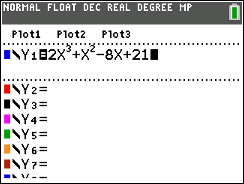
\includegraphics[width=\widthscreens]{screen01}}
&&
{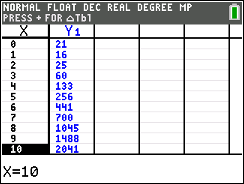
\includegraphics[width=\widthscreens]{screen02}}
&&
{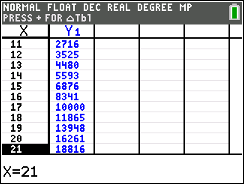
\includegraphics[width=\widthscreens]{screen03}}
&&
{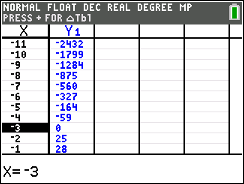
\includegraphics[width=\widthscreens]{screen04}}
&
\end{tabularx}
\setlength{\tabcolsep}{6pt}
}
\end{example}

\begin{example} 
We ontbinden de volgende veelterm zo ver als mogelijk.
\renewcommand{\kolbreed}{\widthof{$-18$}}
\begin{align*}
A(x) & = x^3 + 4x^2 - 3x - 18 \\
& \qquad
\begin{array}{|l}
\hline
\vrule height 0.5cm width 0cm
\text{ kanshebbers gehele nulwaarden: delers van de constante term $-18$
} \\[0.1cm]
\text{ ICT: } A(2) = 0 \text{ en } A(-3) = 0 \text{ dus $A(x)$ is deelbaar door $(x-2)(x+3)$} \\[0.1cm]
\text{ schema's van Horner:} \\[0.1cm]
\qquad
\begin{array}{c|HHHH}
  & 1 & 4 & -3 & -18 \\[0.2cm]
2 & \downarrow  & 2  & 12  & 18  \\[0.2cm]
\hline 
\vrule height 1.2em width 0pt 
  & 1 & 6 & 9 & \multicolumn{1}{|c}{0} \\[0.2cm]
-3& \downarrow & -3 & -9 \\[0.2cm]
\cline{1-4}
\vrule height 1.2em width 0pt
  & 1 & 3 & \multicolumn{1}{|c}{0} 
\end{array} \\[-0.2cm]
\mbox{}\\
\hline
\end{array} \\[0.1cm]
& = (x-2)(x^2+6x+9) \\
& = (x-2)(x+3)(x+3) = (x-2)(x+3)^2
\end{align*}
\end{example}

%%% \clearpage

\begin{example} 
We ontbinden de volgende veelterm zo ver als mogelijk.
\renewcommand{\kolbreed}{\widthof{$-6$}}
\begin{align*}
& \mph{=} \frac{1}{2}\,x^4 + x^3 - x^2 - 3x - \frac{3}{2} \\
& = \frac{1}{2}\underbrace{\left(x^4 + 2x^3 - 2x^2 - 6x - 3 \right)}_{A(x)} \\
& \qquad
\begin{array}{|l}
\hline
\vrule height 0.5cm width 0cm
\text{ kanshebbers gehele nulwaarden: delers van de constante term $-3$
} \\[0.1cm]
\text{ ICT: } A(-1) = 0 \text{ dus $A(x)$ is deelbaar door $x+1$} \\[0.1cm]
\text{ schema van Horner:} \\[0.1cm]
\qquad
\begin{array}{c|HHHHH}
  & 1 & 2 & -2 & -6 & -3 \\[0.2cm]
\D -1 & \downarrow  & -1  & -1  & 3 & 3  \\[0.2cm]
\hline 
\vrule height 1.2em width 0pt 
  & 1 & 1 & -3 & -3 & \multicolumn{1}{|c}{0}
\end{array} \\[-0.2cm]
\mbox{}\\
\hline
\end{array} \\[0.1cm]
& = \frac{1}{2}(x+1)\underbrace{(x^3+x^2-3x-3)}_{Q(x)} \\
& \qquad
\begin{array}{|l}
\hline
\vrule height 0.5cm width 0cm
\text{ kanshebbers gehele nulwaarden: delers van de constante term $-3$
} \\[0.1cm]
\text{ ICT: } Q(-1) = 0 \text{ dus $Q(x)$ is deelbaar door $x+1$} \\[0.1cm]
\text{ schema van Horner:} \\[0.1cm]
\qquad
\begin{array}{c|HHHH}
  & 1 & 1 & -3 & -3 \\[0.2cm]
\D -1 & \downarrow  & -1  & 0  & 3  \\[0.2cm]
\hline 
\vrule height 1.2em width 0pt 
  & 1 & 0 & -3 & \multicolumn{1}{|c}{0}
\end{array} \\[-0.2cm]
\mbox{}\\
\hline
\end{array} \\[0.1cm]
& = \frac{1}{2}(x+1)(x+1)(x^2-3) \\
& = \frac{1}{2}(x+1)^2(x-\sqrt{3})(x+\sqrt{3})
\end{align*}
\end{example}
Vinden we slechts \'e\'en gehele nulwaarde $a$, dan kun je overwegen om  het schema van Horner meteen twee keer na elkaar uit te voeren. Is ook bij het tweede schema de rest gelijk aan nul, dan is de veelterm deelbaar door $(x-a)^2$. Bij het voorbeeld hierboven gaat dat als volgt.
\renewcommand{\kolbreed}{\widthof{$-6$}}
\begin{align*}
A(x) & = x^4 + 2x^3 - 2x^2 - 6x - 3 \\
& \qquad
\begin{array}{|l}
\hline
\vrule height 0.5cm width 0cm
\text{ kanshebbers gehele nulwaarden: delers van de constante term $-3$
} \\[0.1cm]
\text{ ICT: } A(-1) = 0 \text{ dus $A(x)$ is deelbaar door $x+1$} \\[0.1cm]
\text{ schema's van Horner:} \\[0.1cm]
\qquad
\begin{array}{c|HHHHH}
  & 1 & 2 & -2 & -6 & -3 \\[0.2cm]
\D -1 & \downarrow  & -1  & -1  & 3 & 3  \\[0.2cm]
\hline 
\vrule height 1.2em width 0pt 
  & 1 & 1 & -3 & -3 & \multicolumn{1}{|c}{0} \\[0.2cm]
-1 & \downarrow  & -1  & 0  & 3 \\[0.2cm]
\cline{1-5}
\vrule height 1.2em width 0pt 
  & 1 & 0 & -3 & \multicolumn{1}{|c}{0}
\end{array}\\[-0.2cm]
\mbox{}\\
\hline
\end{array} \\[0.1cm]
& = (x+1)(x+1)(x^2-3)
\end{align*}

%%% \clearpage

\section{Algebra\"isch bepalen van nulwaarden}\index{veelterm!nulwaarde} 

Om de nulwaarden van een veelterm $A(x)$ te bepalen, moeten we een \wsgref{vergelijking oplossen}{104}{104}, namelijk $A(x) = 0$. Ontbinden in factoren is een strategie om zo'n vergelijking algebra\"isch op te lossen, want 
uit Eigenschap \ref{eigenschap:geennuldelers} volgt voor elke twee veeltermen $A(x)$ en $B(x)$:
\[
A(x) \cdot B(x) = 0 \quad \Leftrightarrow \quad A(x) = 0 \,\, \text{ of } \,\, B(x)=0. 
\]  

\begin{example}
We bepalen telkens algebra\"isch de nulwaarden van de veelterm.
\begin{enumerate}

\item
$\D \mph{\Leftrightarrow \quad} x^4-34x^2-2x^3-2x-35 = 0$ 
\item[]
$\D \Leftrightarrow \quad \underbrace{x^4 - 2x^3 - 34x^2 - 2x - 35}_{A(x)} = 0$ \quad termen herschikken
\item[]
\renewcommand{\kolbreed}{\widthof{$-35$}}
$\D \mph{\Leftrightarrow \quad}
\begin{array}{|l}
\hline
\vrule height 0.5cm width 0cm
\text{ kanshebbers gehele nulwaarden: delers van de constante term $-35$
} \\[0.1cm]
\text{ ICT: } A(7) = 0 \text{ en } A(-5) = 0 \text{ dus $A(x)$ is deelbaar door $(x-7)(x+5)$} \\[0.1cm]
\text{ schema's van Horner:} \\[0.1cm]
\qquad
\begin{array}{c|HHHHH}
  & 1 & -2 & -34 & -2 & -35 \\[0.2cm]
7 & \downarrow  & 7  & 35  & 7 & 35  \\[0.2cm]
\hline 
\vrule height 1.2em width 0pt 
  & 1 & 5 & 1 & 5 & \multicolumn{1}{|c}{0} \\[0.2cm]
-5& \downarrow & -5 & 0 & -5 \\[0.2cm]
\cline{1-5}
\vrule height 1.2em width 0pt
  & 1 & 0 & 1 & \multicolumn{1}{|c}{0} 
\end{array} \\[-0.2cm]
\mbox{}\\
\hline
\end{array}
$ 
\item[]
$\D \Leftrightarrow \quad (x-7)(x+5)(x^2+1) = 0$
\item[]
$\D \Leftrightarrow \quad x - 7 = 0 \,\, \text{ of } \,\,  x + 5 = 0 \,\, \text{ of } \,\, x^2 + 1 = 0$
\item[]
$\D \Leftrightarrow \quad x = 7 \,\, \text{ of } \,\,  x = -5 \,\, \text{ of } \,\, \underbrace{x^2}_{\geq 0} = \underbrace{-1}_{< 0}$ 
\quad oplossingsverzameling $V = \{7,-5\}$
\item
$\D \mph{\Leftrightarrow \quad} \frac{1}{25}\,x^4-\frac{9}{25}\,x^3+\frac{14}{25}\,x^2+\frac{7}{5}\,x-1 = 0$ 
\item[]
$\D \Leftrightarrow \quad \underbrace{x^4 - 9x^3 + 14x^2 + 35x - 25}_{A(x)} = 0$ \quad beide leden maal $25$
\item[]
\renewcommand{\kolbreed}{\widthof{$-25$}}
$\D \mph{\Leftrightarrow \quad}
\begin{array}{|l}
\hline
\vrule height 0.5cm width 0cm
\text{ kanshebbers gehele nulwaarden: delers van de constante term $-25$
} \\[0.1cm]
\text{ ICT: } A(5) = 0 \text{ dus $A(x)$ is deelbaar door $x-5$} \\[0.1cm]
\text{ schema's van Horner:} \\[0.1cm]
\qquad
\begin{array}{c|HHHHH}
  & 1 & -9 & 14 & 35 & -25 \\[0.2cm]
5 & \downarrow  & 5  & -20  & -30 & 25  \\[0.2cm]
\hline 
\vrule height 1.2em width 0pt 
  & 1 & -4 & -6 & 5 & \multicolumn{1}{|c}{0} \\[0.2cm]
5 & \downarrow & 5 & 5 & -5 \\[0.2cm]
\cline{1-5}
\vrule height 1.2em width 0pt
  & 1 & 1 & -1 & \multicolumn{1}{|c}{0} 
\end{array} \\[-0.2cm]
\mbox{}\\
\hline
\end{array}
$ 
\item[]
$\D \Leftrightarrow \quad (x-5)^2(x^2+x-1) = 0$
\item[]
$\D \Leftrightarrow \quad x - 5 = 0 \,\, \text{ of } \,\,  x^2+x-1 = 0$
\item[]
$\D \Leftrightarrow \quad x = 5 \,\, \text{ of } \,\,  x = \frac{-1 \pm \sqrt{5}}{2}$ \quad oplossingsverzameling $\D V = \left\{5,\frac{-1 + \sqrt{5}}{2},\frac{-1 - \sqrt{5}}{2} \right\}$
\end{enumerate}
\end{example}

%%% \clearpage

\begin{Uitbreiding}
Elke veelterm $A(x)$ kan opgevat worden als het voorschrift van een functie, waarvan we de grafiek kunnen plotten. De snijpunten van die grafiek met de $x$-as komen dan overeen met de oplossingen van de vergelijking $A(x) = 0$, en dus met de nulwaarden van de veelterm. De ontbinding in factoren geeft de ligging van de grafiek ten opzichte van de $x$-as aan, en in welke punten de grafiek raakt aan de $x$-as. 

\begin{example}
Gegeven is de functie $f$ met als voorschrift $f(x) = x^4 + x^3 - 13x^2-x$ waarvan de grafiek hieronder staat afgebeeld. Er worden ook drie snijpunten van de grafiek met de $x$-as aangeduid: de oorsprong $O$ en de punten $P$ en $Q$. 

\medskip

%%%%%%%%%%%%%%%%%%%%%%%%%%%%%%%%%%%%%%%%%%%%%%%%%%%%%%%%%%%%%%%%%%%%%%%%%
\begin{center}
\psset{xunit=0.525cm,yunit=0.525cm}
\begin{pspicture}(-4.5,-4.99)(4,5.7) % co linksonder, co rechtsboven
\psaxes[labels=none,ticks=none]{->}(0,0)(-4.5,-4.99)(4,5.7)
\uput[l](0,5.7){$y$}
\uput[d](4,0){$x$}
\psplot[plotpoints=200,linewidth=0.4mm,linecolor=graf]{-4.5}{3.85}{x 4 add x 1 add mul x 1 neg add mul x 3 neg add mul 14 div 0.5 add 19 14 div neg add}
\uput[r](-4.5,5){\color{graf} $f$}
\uput[ur](0,0){$O$}
\psline[linewidth=0.4mm,linecolor=graf]{*-*}(0,0)(0,0)
\uput[ur](-4.1064,0){$P$}
\psline[linewidth=0.4mm,linecolor=graf]{*-*}(-4.1064,0)(-4.1064,0)
\uput[ul](3.1829,0){$Q$}
\psline[linewidth=0.4mm,linecolor=graf]{*-*}(3.1829,0)(3.1829,0)
\end{pspicture}
\end{center}
%%%%%%%%%%%%%%%%%%%%%%%%%%%%%%%%%%%%%%%%%%%%%%%%%%%%%%%%%%%%%%%%%%%%%%%%%

Het lijkt het erop dat de punten $O$, $P$ en $Q$ de enige snijpunten van de grafiek met de $x$-as zijn. Meer bepaald, we hebben de indruk dat de grafiek van $f$ de $x$-as raakt in de oorsprong. Schrijven we $\co(P) = (a,0)$ en $\co(Q) = (b,0)$ met $a,b \in \RR$ dan vermoeden we dat de tekentabel van $f$ gegeven wordt door
\renewcommand{\kolbreed}{\widthof{$a$}}
\[
\begin{array}{c|HHHHHHH}
x  & & a &  & 0 & & b & \\
\hline 
\vrule height 1.2em width 0pt 
f(x) & + & 0 & - & 0 & - & 0 & +
\end{array} 
\]
Om dat met zekerheid te weten, redeneren we als volgt. Alvast is 
\[
f(x) = x(x^3 + x^2 - 13x - 1)
\]
zodat $f(0) = 0$, en de grafiek van $f$ de $x$-as snijdt in de oorsprong.  Omdat $f(a) = 0$ weten we dat $f(x)$ deelbaar is door $x-a$. Analoog is $f(x)$ ook deelbaar door $x-b$. Hieruit volgt dat 
\[
f(x) = x(x-a)(x-b)(x-c)
\]
voor een zeker re\"eel getal $c$, en omdat $abc = 1$ en $a < 0$ en $b > 0$ weten we dat $c < 0$. Naast de drie snijpunten $O(0,0)$, $P(a,0)$ en $Q(b,0)$ is er dus nog een vierde snijpunt $R(c,0)$ van de grafiek van $f$ met de $x$-as, die zich net links van de $y$-as situeert. De correcte tekentabel van de functie $f$ wordt dus gegeven door
\renewcommand{\kolbreed}{\widthof{$a$}}
\[
\begin{array}{c|HHHHHHHHH}
x  & & a & & c & & 0 & & b & \\
\hline 
\vrule height 1.2em width 0pt 
f(x) & + & 0 & - & 0 & + & 0 & - & 0 & +
\end{array} 
\]
Ter controle gebruiken we ICT om de veelterm $x^4 + x^3 - 13x^2-x$ te ontbinden in factoren:
\[
f(x) = x(x+4,1064\ldots)(x-3,1829\ldots)(x+0,0765\ldots).
\]
De reden waarom de grafiek van $f$ de $x$-as snijdt in de oosprong maar niet raakt in de oorsprong, is omdat $f(x)$ deelbaar is door $x-0$, maar niet door $(x-0)^2$. 
\end{example}
\end{Uitbreiding}

%%% \clearpage

\phantomsection
\addcontentsline{toc}{section}{Oefeningen}

\section*{Oefeningen reeks 1}
\begin{Oefening}[\bf \ref{antw4.1}.]\setcounter{enumi}{1}
\hypertarget{oef4.1}{Werk} telkens de veelterm uit. Vereenvoudig zoveel mogelijk. 
\begin{multicols}{2}
\begin{enumerate}

\item
$-3x^7\left(-7x^3\right)$
\item
$\D \frac{3}{10}\,x^5\left(-\frac{3}{5}x^2\right)$
\item
$\D -\frac{1}{2}\,x^2\left(x^4-6x^3-8x^2+2x-1\right)$
\item
$(x-1)^3(x-1)^2$
\end{enumerate}
\end{multicols}
\end{Oefening}

\begin{Oefening}[\bf \ref{antw4.2}.]\setcounter{enumi}{2}
\hypertarget{oef4.2}{Werk} telkens de veelterm uit met behulp van merkwaardige producten. Vereenvoudig zoveel mogelijk. 
\begin{multicols}{2}
\begin{enumerate}

\item
$(\sqrt{3}\,x-2)(\sqrt{3}\,x+2)$
\item
$(x^2-1)(x^2+1)$
\item
$(-x^3-3)(-x^3+3)$
\item
$\D \left(-2x^3-\frac{1}{3}\right)^2$
\item
$(1+x+x^2)(1+x-x^2)$
\item
$(x^6-x^3+1)(x^6+x^3-1)$
\item
$(x^2-2x+5)^2$
\item
$\D \left(-\frac{1}{2}\,x^3 - \frac{2}{3}\,x^2-\frac{2}{5}\right)^2$
\end{enumerate}
\end{multicols}
\end{Oefening}

\begin{Oefening}[\bf \ref{antw4.3}.]\setcounter{enumi}{3} 
\hypertarget{oef4.3}{Ontbind} telkens de veelterm zo ver mogelijk in factoren. Ga algebra\"isch te werk en schrijf jouw redenering uit.  
\begin{multicols}{2}
\begin{enumerate}

\item
$1000 x^3 + 1$
\item
$8x^3-216$
\item
$-81x^2+72x-16$
\item
$x^4-4x^3+4x^2$
\item
$-17x+38$
\item
$(x-3)(5x^2+50x+110)$
\end{enumerate}
\end{multicols}
\end{Oefening}

\begin{Oefening}[\bf \ref{antw4.4}.]\setcounter{enumi}{4}
\hypertarget{oef4.4}{Ontbind} telkens de veelterm zo ver mogelijk in factoren. Ga algebra\"isch te werk en schrijf jouw redenering uit.  
\begin{multicols}{2}
\begin{enumerate}

\item
$x^3+2x^2-2x-3$
\item
$x^5+7x^4+10x^3-18x^2-27x+27$
\item 
$\D x^4-544x^3+1626x^2-1624x+541 \mph{\frac{2}{3}}$
\item
$6x^4 + 4x^3 - 26x^2 - 16x + 8$
\item
$21-40x^2-21x^4$
\item
$\D \frac{2}{3}\,x^4-\frac{5}{3}\,x^2 + x^3 - 3x-1$
\end{enumerate}
\end{multicols}
\end{Oefening}

\section*{Oefeningen reeks 2}

\begin{Oefening}[\bf \ref{antw4.5}.]\setcounter{enumi}{5} 
\hypertarget{oef4.5}{Ontbind} telkens de veelterm zo ver mogelijk in factoren. Ga algebra\"isch te werk en schrijf jouw redenering uit.  
\begin{multicols}{2}
\begin{enumerate}

\item
$6x^2+x-15$
\item
$\D \frac{1}{27} - \frac{x^3}{8}$
\item
$2x^5-7x^4-38x^3$
\item
$2x^2 - 6073x + 4\,098\,600$
\item
$\D 1-x^2+\frac{1}{4}\,x^4$
\item
$2x^3 - 15x^2 + 19x - 6$
\end{enumerate}
\end{multicols}
\end{Oefening}

\begin{Oefening}[\bf \ref{antw4.6}.]\setcounter{enumi}{6}  
\hypertarget{oef4.6}{Bepaal} telkens algebra\"isch alle nulwaarden van de veelterm. Schrijf jouw redenering uit.
\begin{multicols}{2}
\begin{enumerate}
\item
$3x^2-11\sqrt{3}\,x+30$
\item
$12x^4-5x^3-28x^2$
\item
$x^3-5x+4$
\item
$2x^3 - 5x^2 - 39x - 18$
\item
$x^4+8x^3+17x^2-6x-36$
\item
$2x^3+x^2-17x-12$ 
\item
$3x^5-30x^4+120x^3-240x^2+240x-96$
\item
$x^3 - 3\sqrt{2}\,x^2 + 6x - 2\sqrt{2}\,$
\end{enumerate}
\end{multicols}
\end{Oefening}

\begin{Oefening}[\bf \ref{antw4.7}.]\setcounter{enumi}{7}   
\hypertarget{oef4.7}{Gegeven} is de veelterm
\[
A(x) = 3x^4-21x^2-7x^3+35x+30.
\]
Er is ook gegeven dat de getalwaarde van $A(x)$ in $\D x = -\frac{2}{3}$ gelijk is aan nul. Bepaal algebra\"isch alle nulwaarden van de veelterm $A(x)$.
\end{Oefening}

\begin{Oefening}[\bf \ref{antw4.8}.]\setcounter{enumi}{8}
\hypertarget{oef4.8}{Beschouw} de veelterm
\[
P(x) = 3x^3-20x^2+kx+12
\]
waarbij $k \in \RR$. Er gegeven dat $P(x)$ deelbaar is door $x-3$. Bepaal algebra\"isch alle nulwaarden van de veelterm $P(x)$.
\end{Oefening}

\section*{Oefeningen reeks 3}

\begin{Oefening}[\bf \ref{antw4.9}.]\setcounter{enumi}{9}
\hypertarget{oef4.9}{Bepaal} alle kubische veeltermen $A(x)$ waarvan de constante term gelijk is aan nul en waarvoor geldt dat
\[
A(x) - A(x-1) = x^2.
\]
\end{Oefening}

\begin{Uitbreiding}
\begin{Oefening}[\bf \ref{antw4.10}.]\setcounter{enumi}{10}
\hypertarget{oef4.10}{In} wiskunde staat een \underline{bewijs zonder woorden}\index{bewijs zonder woorden} voor een figuur die aangeeft dat een bepaalde wiskundige uitspraak vanzelfsprekend is, zonder dat daarbij begeleidende uitleg vermeld wordt. Daarbij gaat het vaak om identiteiten in de algebra of stellingen in de meetkunde. Zo werden al bewijzen zonder woorden gevonden van de stelling van Pythagoras, de cosinusregel en formules voor sommen van getallen die aan een bepaalde regelmaat voldoen, zoals de eindige som 
\[
1 + 2 + 3 + \dots + n 
\]
met $n \in \NN_0$ willekeurig, en de niet-eindigende sommen 
\[
0,9 + 0,09 + 0,009 + \dots \quad \text{ en } \quad 1 + \frac{1}{2} + \frac{1}{4} + \frac{1}{8} + \dots
\]
Een bewijs zonder woorden geldt niet als een volledig bewijs zoals we dat in wiskunde kennen, omdat de logische argumenten ontbreken om de uitspraak formeel aan te tonen. Het kan wel waardevolle intu\"itieve ide\"een aanreiken. Op die manier kan er voor elk bewijs zonder woorden een redenering worden opgeschreven die gebaseerd is op de figuur en die kan gelden als een volledig bewijs van de uitspraak. 

Hieronder staat een bewijs zonder woorden van een merkwaardig product. Formuleer de bijbehorende uitspraak en schrijf op basis van de figuur een volledig bewijs op.

\medskip

%%%%%%%%%%%%%%%%%%%%%%%%%%%%%%%%%%%%%%%%%%%%%%%%%%%%%%%%%%%%%%%%%%%%%%%%%
\begin{center}
\psset{xunit=0.75cm,yunit=0.75cm}
\begin{pspicture}(2.5,0)(8,5.5) % co linksonder, co rechtsboven

\psline[](3,0)(8,0)(8,5)(3,5)(3,0)

\psline[](3,1)(8,1)
\psline[](7,0)(7,5)

\uput[u](7.5,0.2){$b^2$}
\uput[u](5,0.2){$ab$}
\uput[u](7.5,2.7){$ab$}
\uput[u](5,2.7){$a^2$}

\uput[u](2.7,2.7){$a$}
\uput[u](2.7,0.2){$b$}

\uput[u](5,5){$a$}
\uput[u](7.5,5){$b$}
\end{pspicture}
\end{center}
%%%%%%%%%%%%%%%%%%%%%%%%%%%%%%%%%%%%%%%%%%%%%%%%%%%%%%%%%%%%%%%%%%%%%%%%%
\end{Oefening}
\end{Uitbreiding}

%%% \clearpage

\begin{Oefening}[\bf \ref{antw4.11}.]\setcounter{enumi}{11} 
\hypertarget{oef4.11}{Ontbind} telkens de veelterm zo ver mogelijk in factoren. Ga algebra\"isch te werk en schrijf jouw redenering uit.  
\begin{multicols}{2}
\begin{enumerate}

\item
$x^4+1$
\item
$x^4 + x^2 + 1$
\item
$x^5-1$
\item
$x^5+1$
\end{enumerate}
\end{multicols}
\end{Oefening}

\begin{Oefening}
Zij $A(x)$ een willekeurige veelterm met gehele co\"effici\"enten en met hoogstegraadsco\"effici\"ent gelijk aan $1$. Toon aan: als $A(x)$ een rationale nulwaarde heeft, dan heeft $A(x)$ ook een gehele nulwaarde.
\end{Oefening}

\begin{Uitbreiding}
\begin{Oefening}
Toon telkens de veeltermgelijkheid aan. Hierbij is $a$ een willekeurig re\"eel getal en $n \in \NN_0$.
\begin{enumerate}

\item
$\D x^{n+1} - a^{n+1} = (x-a)(x^{n} + ax^{n-1} + a^2x^{n-2} + \dots + a^{n-2}x^2 + a^{n-1}x + a^{n})$
\item
$\D x^{2n+1} + a^{2n+1} = (x+a)(x^{2n} - ax^{2n-1} + a^2x^{2n-2} - a^3x^{2n-3} + \dots - a^{2n-1}x + a^{2n})$
\end{enumerate}
\end{Oefening}

\begin{Oefening}
\label{somtweevierdemachten}
Toon voor elke $a \in \RR_0$ aan dat het zo ver mogelijk ontbinden in factoren van de veeltermen $x^2 \pm a^2$, $x^3 \pm a^3$, $x^4 \pm a^4$ en  $x^5 \pm a^5$ wordt gegeven door onderstaande uitdrukkingen. Hierbij staat $\varphi$ voor de gulden snede. %{\wsgref{gulden snede}{Bijzondere irrationale getallen}{22}}. 
\begin{align*}
& x^2 + a^2 = x^2 + a^2 && \text{som van twee kwadraten} \\
& x^2 - a^2 = (x-a)(x+a) && \text{verschil van twee kwadraten} \\
& x^3 + a^3 = (x+a)(x^2 - ax + a^2) && \text{som van twee derde machten} \\
& x^3 - a^3 = (x-a)(x^2 + ax + a^2) && \text{verschil van twee derde machten} \\
& x^4 + a^4 = (x^2 + \sqrt{2}\,ax + a^2)(x^2 - \sqrt{2}\,ax + a^2) && \text{som van twee vierde machten} \\
& x^4 - a^4 = (x-a)(x+a)(x^2+a^2) && \text{verschil van twee vierde machten} \\
& x^5 + a^5 = (x+a)(x^2-\varphi\,ax + a^2)(x^2+\frac{1}{\varphi}\,ax + a^2) && \text{som van twee vijfde machten} \\
& x^5 - a^5 = (x-a)(x^2+\varphi\,ax + a^2)(x^2-\frac{1}{\varphi}\,ax + a^2) && \text{verschil van twee vijfde machten}
\end{align*}
\end{Oefening}

\begin{Oefening}\label{oefening:gehelewortelstelling}
{\bf (gehele wortelstelling)}\index{gehele wortelstelling} 
In deze oefening bewijzen we de Stelling \ref{stelling:gehelewortelstelling}: 
\begin{itemize}
\item[]
Zij $A(x)$ een veelterm met gehele co\"effici\"enten. Als $a \neq 0$ een gehele nulwaarde van $A(x)$ is, dan is $a$ een deler van de constante term.
\end{itemize}
Beschouw een willekeurige veelterm met gehele co\"effici\"enten:
\[
A(x) = a_0 + a_1 x + a_2 x^2 + \dots + a_{n-1} x^{n-1} + a_nx^n
\]
waarbij $ n \in \NN$ en $a_0, a_1, \ldots, a_n \in \ZZ$. Stel nu dat $a \neq 0$ een gehele nulwaarde van deze veelterm is, dus
\[
a \in \ZZ_0 \quad \text{ en } \quad A(a) = 0.
\]
Toon aan dat $A(a) = 0$ leidt tot $a_0 = a\cdot q$ voor een zeker geheel getal $q$, en dus dat $a \mid a_0$. 
\end{Oefening}
\end{Uitbreiding}

%%% \clearpage

\begin{Uitbreiding}
\begin{Oefening}\label{oefening:rationalewortelstelling}
{\bf (rationale wortelstelling)}\index{rationale wortelstelling} 
In deze oefening bewijzen we de rationale wortelstelling:
\begin{itemize}
\item[]
Zij $A(x)$ een veelterm met gehele co\"effici\"enten. Als $\frac{p}{q} \neq 0$ een rationale nulwaarde van $A(x)$ is (met $p,q$ gehele getallen en $\frac{p}{q}$ onvereenvoudigbaar), dan is $p$ een deler van de constante term en $q$ een deler van de hoogstegraadsco\"effici\"ent  
\end{itemize}
Beschouw een willekeurige veelterm met gehele co\"effici\"enten:
Beschouw een willekeurige veelterm met gehele co\"effici\"enten:
\[
A(x) = a_0 + a_1 x + a_2 x^2 + \dots + a_{n-1} x^{n-1} + a_nx^n
\]
waarbij $ n \in \NN$ en $a_0, a_1, \ldots, a_n \in \ZZ$. Beschouw nu een rationaal getal $\frac{p}{q} \neq 0$, en stel dat dit getal een nulwaarde van deze veelterm is waarbij $p,q$ gehele getallen en $\frac{p}{q}$ onvereenvoudigbaar, dus
\[
p,q \in \ZZ_0 \quad \text{ en } \quad \ggd(p,q)=1 \quad \text{ en } \quad A\left(\frac{p}{q}\right) = 0.
\]
Toon aan dat $A\left(\frac{p}{q}\right) = 0$ leidt tot $p \mid a_0q^n$ en $q \mid a_n p^n$, en dus tot $p \mid a_0$ en $q \mid a_n$.
\end{Oefening}
\end{Uitbreiding}

\begin{Oefening}[\bf \ref{antw4.17}.]\setcounter{enumi}{17} 
\hypertarget{oef4.17}{Bepaal} algebra\"isch alle re\"ele getallen $x$ waarvoor geldt dat 
\[
x^3-288x^2-282x  = 2023.
\]
Schrijf alle tussenstappen op.
\end{Oefening}

\begin{Oefening}[\bf \ref{antw4.18}.]\setcounter{enumi}{18} 
\hypertarget{oef4.18}{Bepaal} algebra\"isch alle nulwaarden van de veelterm
\[
A(x) = x^6 + x^4 + x^2 + 1.
\]
Schrijf alle tussenstappen op.
\end{Oefening}

\begin{Oefening}[\bf \ref{antw4.19}.]\setcounter{enumi}{19} 
\hypertarget{oef4.19}{Bepaal} een veelterm met gehele co\"effici\"enten waarvan $\sqrt{3+\sqrt{17}}$ een nulwaarde is.
\end{Oefening}

\begin{Uitbreiding}
\begin{Oefening}
In deze oefening laten we zien dat de rationale wortelstelling (zie Oefening \ref{oefening:rationalewortelstelling}) gebruikt kan worden om aan te tonen dat sommige re\"eele getallen irrationaal zijn.
\begin{enumerate}

\item
Bepaal een veelterm $A(x)$ met gehele co\"effici\"enten waarvan $\sqrt{2}$ een nulwaarde is.
\item
Toon met behulp van de rationale wortelstelling aan dat die veelterm $A(x)$ geen rationale nulwaarden heeft.
\item
Argumenteer nu hoe uit (a) en (b) volgt dat $\sqrt{2}$ een irrationaal getal is.
\item
Toon op een gelijkaardige manier aan dat de volgende re\"ele getallen irrationaal zijn:
\[
\sqrt{17}, \qquad \sqrt[3]{2}, \qquad \sqrt[7]{13} \qquad \sqrt{3+\sqrt{17}}, 
\qquad \text{ en } \qquad \sqrt{2}+\sqrt{3}.
\]
\end{enumerate}
\end{Oefening}
\end{Uitbreiding}

%%% \clearpage

%%% \backmatter

\chapter{Eindantwoorden van oefeningen}
\section*{Hoofdstuk 1}

\begin{Antwoord} \label{antw1.1}
\begin{enumerate}

\item
\hyperlink{oef1.1}{eenterm}
\item
\hyperlink{oef1.1}{eenterm}
\item
\hyperlink{oef1.1}{geen eenterm}
\item
\hyperlink{oef1.1}{eenterm}
\item
\hyperlink{oef1.1}{geen eenterm}
\item
\hyperlink{oef1.1}{eenterm}
\item\hyperlink{oef1.1}{eenterm}
\item
\hyperlink{oef1.1}{eenterm}
\item
\hyperlink{oef1.1}{geen eenterm}
\item
\hyperlink{oef1.1}{geen eenterm}
\end{enumerate}
\end{Antwoord}

\begin{Antwoord} \label{antw1.2}
\begin{enumerate}
\item
\hyperlink{oef1.2}{$x + 2x^2 + 3x^3$}
\item
\hyperlink{oef1.2}{$x + \frac{1}{2}\,x^3 + \frac{1}{3}\,x^5 + \frac{1}{4}\,x^7$}
\item
\hyperlink{oef1.2}{$x^2 - x^3 + x^4$}
\end{enumerate}
\end{Antwoord}

\begin{Antwoord} \label{antw1.3}
\begin{enumerate}
\item
\hyperlink{oef1.3}{veelterm}
\item
\hyperlink{oef1.3}{veelterm}
\item
\hyperlink{oef1.3}{veelterm}
\item
\hyperlink{oef1.3}{veelterm}
\item
\hyperlink{oef1.3}{veelterm}
\item
\hyperlink{oef1.3}{veelterm}
\item
\hyperlink{oef1.3}{geen veelterm}
\item
\hyperlink{oef1.3}{veelterm}
\item
\hyperlink{oef1.3}{veelterm}
\item
\hyperlink{oef1.3}{geen veelterm}
\item
\hyperlink{oef1.3}{veelterm}
\item
\hyperlink{oef1.3}{veelterm}
\end{enumerate}
\setcounter{enumi}{4}
\end{Antwoord}

%%% \clearpage

\begin{Antwoord} \label{antw1.5}
\begin{enumerate}
\item
\hyperlink{oef1.5}{graad $5$, hoogstegraadsco\"effici\"ent $1$, constante term $-15$}
\item
\hyperlink{oef1.5}{graad $6$, hoogstegraadsco\"effici\"ent $2$, constante term $3$}
\item
\hyperlink{oef1.5}{graad $7$, hoogstegraadsco\"effici\"ent $\frac{2}{3}$, constante term $-\frac{3}{7}$}
\item
\hyperlink{oef1.5}{graad $6$, hoogstegraadsco\"effici\"ent $-15$, constante term $-70$}
\item
\hyperlink{oef1.5}{graad $3$, hoogstegraadsco\"effici\"ent $125$, constante term $0$}
\item
\hyperlink{oef1.5}{graad $6$, hoogstegraadsco\"effici\"ent $64$, constante term $125$}
\end{enumerate}
\setcounter{enumi}{6}
\end{Antwoord}

\begin{Antwoord} \label{antw1.7}
\begin{enumerate}
\item
\hyperlink{oef1.7}{$-x^3+x^2+3x+1$, graad $3$}
\item
\hyperlink{oef1.7}{$x^3-5x^2+4x$, graad $3$}
\item
\hyperlink{oef1.7}{$\sqrt{10}\,x+\sqrt{15}$, graad $1$}
\item
\hyperlink{oef1.7}{$-9x^4+45x^3+3x^2-21x+30$, graad $4$}
\item
\hyperlink{oef1.7}{$-\frac{4}{5}\,x^2-\frac{1}{5}\,x-\frac{4}{5}$, graad $2$}
\item
\hyperlink{oef1.7}{$4x-8$, graad $1$}
\item
\hyperlink{oef1.7}{$-8x^2+18$, graad $2$}
\item
\hyperlink{oef1.7}{$\frac{15}{2}\,x^3 + 3x^2 - \frac{10}{3}\,x-\frac{4}{3}$, graad $3$}
\end{enumerate}
\end{Antwoord}

\begin{Antwoord} \label{antw1.8}
\begin{enumerate}
\item
\hyperlink{oef1.8}{$A(2)=0$, nulwaarde}
\item
\hyperlink{oef1.8}{$B(-1)=1$, geen nulwaarde}
\item
\hyperlink{oef1.8}{$P(5)=0$, nulwaarde}
\item
\hyperlink{oef1.8}{$S(0)=-1$, geen nulwaarde}
\item
\hyperlink{oef1.8}{$C(\sqrt{2})=0$, nulwaarde}
\item
\hyperlink{oef1.8}{$D\left(-\frac{1}{2}\right)=0$, nulwaarde}
\end{enumerate}
\end{Antwoord}

\begin{Antwoord} \label{antw1.9}
\begin{enumerate}
\item
\hyperlink{oef1.9}{$a=-3$}
\item
\hyperlink{oef1.9}{$a = 1$ en $b = -3$}
\end{enumerate}
\end{Antwoord}

\begin{Antwoord} \label{antw1.10}
\begin{enumerate}
\item
\hyperlink{oef1.10}{$a = -\frac{3}{2}$}
\item
\hyperlink{oef1.10}{$c = \frac{2}{1-\sqrt{2}}$}
\end{enumerate}
\end{Antwoord}

\begin{Antwoord} \label{antw1.11}
\begin{enumerate}
\item
\hyperlink{oef1.11}{$A(x) = -3x^6+24x^4+12x^2$ en $B(x) = -5x^2$}
\item
\hyperlink{oef1.11}{$\gr A(x) = 6$ en $\gr B(x) = 2$}
\item
\hyperlink{oef1.11}{$A(-2) = 240$ en $B(\sqrt{3}) = -15$}
\end{enumerate}
\end{Antwoord}


\begin{Antwoord} \label{antw1.12}
\begin{enumerate}
\item
\hyperlink{oef1.12}{$475$}
\item
\hyperlink{oef1.12}{$c = -2$}
\end{enumerate}
\end{Antwoord}

\begin{Antwoord} \label{antw1.13}
\hyperlink{oef1.13}{$A(x) = -x^2-x+2$}
\end{Antwoord}

\begin{Antwoord} \label{antw1.14}
\hyperlink{oef1.14}{$A(x) = \frac{1}{3}\,x^3-\frac{1}{3}\,x$}
\end{Antwoord}

\begin{Antwoord} \label{antw1.15}
\hyperlink{oef1.15}{$2x^2+3x+1$}
\end{Antwoord}

\begin{Antwoord} \label{antw1.16}
\hyperlink{oef1.16}{$a = 3$ en $b = \frac{1}{4}$}
\end{Antwoord}

\begin{Antwoord} \label{antw1.17}
\hyperlink{oef1.17}{$4096$}
\end{Antwoord}

\begin{Antwoord} \label{antw1.18}
\hyperlink{oef1.18}{$32$}
\setcounter{enumi}{0}
\end{Antwoord}

%%% \clearpage

\section*{Hoofdstuk 2}

\begin{Antwoord} \label{antw2.1}
\begin{enumerate}

\item
\hyperlink{oef2.1}{deelbaar, quoti\"ent $6x^2$} 
\item
\hyperlink{oef2.1}{deelbaar, quoti\"ent $-2$}
\item
\hyperlink{oef2.1}{deelbaar, quoti\"ent $\frac{3}{2}\,x^4$}
\item
\hyperlink{oef2.1}{deelbaar, quoti\"ent $0$}
\item
\hyperlink{oef2.1}{niet deelbaar}
\item
\hyperlink{oef2.1}{deelbaar, quoti\"ent $-\frac{1}{10}\,x$}
\item
\hyperlink{oef2.1}{deelbaar, quoti\"ent $\frac{\sqrt{2}}{6}$}
\item
\hyperlink{oef2.1}{niet deelbaar}
\end{enumerate}
\end{Antwoord}

\begin{Antwoord} \label{antw2.2}
\begin{enumerate}
\item
\hyperlink{oef2.2}{deelbaar door $6$, quoti\"ent $2x^3 - 3x^2 + x$} 
\item[]
\hyperlink{oef2.2}{deelbaar door $3x$, quoti\"ent $4x^2 - 6x + 2$} 
\item[]
\hyperlink{oef2.2}{niet deelbaar door $3x^2$}
\item
\hyperlink{oef2.2}{deelbaar door $6$, quoti\"ent $x^2 - \frac{1}{2}\,x$} 
\item[]
\hyperlink{oef2.2}{deelbaar door $3x$, quoti\"ent $2x-1$} 
\item[]
\hyperlink{oef2.2}{niet deelbaar door $3x^2$}
\item
\hyperlink{oef2.2}{deelbaar door $6$, quoti\"ent $0$} 
\item[]
\hyperlink{oef2.2}{deelbaar door $3x$, quoti\"ent $0$} 
\item[]
\hyperlink{oef2.2}{niet deelbaar door $0$}
\item
\hyperlink{oef2.2}{deelbaar door $6$, quoti\"ent $\frac{1}{3}\,x^3 + \frac{1}{10}\,x^2$} 
\item[]
\hyperlink{oef2.2}{deelbaar door $3x$, quoti\"ent $\frac{2}{3}\,x^2 + \frac{1}{5}\,x$} 
\item[]
\hyperlink{oef2.2}{deelbaar door $3x^2$, quoti\"ent $\frac{2}{3}\,x + \frac{1}{5}$}
\item
\hyperlink{oef2.2}{deelbaar door $6$, quoti\"ent $\frac{\sqrt{3}}{6}\,x - \frac{4}{3}$} 
\item[]
\hyperlink{oef2.2}{niet deelbaar door $3x$}
\item[]
\hyperlink{oef2.2}{niet deelbaar door $3x^2$}
\item
\hyperlink{oef2.2}{deelbaar door $6$, quoti\"ent $\frac{1}{6}\,x^8 - \frac{\pi}{6}\,x^5$} 
\item[]
\hyperlink{oef2.2}{deelbaar door $3x$, quoti\"ent $\frac{1}{3}\,x^7 - \frac{\pi}{3}\,x^4$} 
\item[]
\hyperlink{oef2.2}{deelbaar door $3x^2$, quoti\"ent $\frac{1}{3}\,x^6 - \frac{\pi}{3}\,x^3$}
\end{enumerate}
\end{Antwoord}

\begin{Antwoord} \label{antw2.3}
\hyperlink{oef2.3}{$-3x^3+11x^2-5x+2$}
\end{Antwoord}

\begin{Antwoord} \label{antw2.4}
\hyperlink{oef2.4}{$p=2$ en $q=8$}
\end{Antwoord}

\begin{Antwoord} \label{antw2.5}
\begin{enumerate}
\item
\hyperlink{oef2.5}{quoti\"ent $5$, rest $3x$, niet deelbaar, verband $A(x) = 5B(x)+3x$}
\item
\hyperlink{oef2.5}{quoti\"ent $x$, rest $0$, deelbaar, verband $A(x) = xB(x)+0$}
\item
\hyperlink{oef2.5}{quoti\"ent $\frac{5}{2}\,x$, rest $2$, niet deelbaar, verband $A(x) = \frac{5}{2}\,xB(x)+2$}
\item
\hyperlink{oef2.5}{quoti\"ent $-\frac{3}{5}$, rest $0$, deelbaar, verband $A(x) = -\frac{3}{5}\,B(x)+0$}
\item
\hyperlink{oef2.5}{quoti\"ent $0$, rest $7x^2-8x+5$, niet deelbaar, verband $A(x) = 0B(x)+7x^2-8x+5$}
\item
\hyperlink{oef2.5}{quoti\"ent $3$, rest $10x-72$, niet deelbaar, verband $A(x) = 3B(x)+10x-72$}
\item
\hyperlink{oef2.5}{quoti\"ent $-\frac{8}{3}\,x$, rest $16$, niet deelbaar, verband $A(x) = -\frac{8}{3}\,xB(x)+16$}
\end{enumerate}
\end{Antwoord}

\begin{Antwoord} \label{antw2.6}
\hyperlink{oef2.6}{$12$}
\end{Antwoord}

\begin{Antwoord} \label{antw2.7}
\begin{enumerate}
\item
\hyperlink{oef2.7}{niet deelbaar}
\item
\hyperlink{oef2.7}{niet deelbaar}
\item
\hyperlink{oef2.7}{deelbaar}
\item
\hyperlink{oef2.7}{deelbaar}
\item
\hyperlink{oef2.7}{niet deelbaar}
\end{enumerate}
\end{Antwoord}

\begin{Antwoord} \label{antw2.8}
\begin{enumerate}
\item
\hyperlink{oef2.8}{$x^4 + x^2 + 1 = (x^2+x+1)(x^2-x+1)$}
\item
\hyperlink{oef2.8}{$x^5 - 1 = (x-1)(x^4+x^3+x^2+x+1)$}
\item
\hyperlink{oef2.8}{$x^4 + 1 = (x^2+\sqrt{2}\,x+1)(x^2-\sqrt{2}\,x+1)$}
\end{enumerate}
\end{Antwoord}

\begin{Antwoord} \label{antw2.9}
\begin{enumerate}
\item
\hyperlink{oef2.9}{$a=2$ en $b = 2$}
\item
\hyperlink{oef2.9}{$a = 22$ en $b = -8$}
\item
\hyperlink{oef2.9}{$a = 0$ en $b = 2$}
\item
\hyperlink{oef2.9}{$a = 4$, $b = 3$ en $c = 5$}
\item
\hyperlink{oef2.9}{$a \in \left\{\sqrt{2},-\sqrt{2}\right\}$ en $b = 1$}
\item
\hyperlink{oef2.9}{$a \in \left\{1,-1\right\}$ en $b = 1$}
\end{enumerate}
\end{Antwoord}

\begin{Antwoord} \label{antw2.10}
\begin{enumerate}
\item
\hyperlink{oef2.10}{quoti\"ent $x-1$, rest $0$, deelbaar, verband $A(x) = (x-1)B(x)+0$}
\item
\hyperlink{oef2.10}{quoti\"ent $-\frac{1}{3}\,x - \frac{4}{3}$, rest $0$, deelbaar, verband $A(x) = \left(-\frac{1}{3}\,x - \frac{4}{3}\right)B(x)+0$}
\item
\hyperlink{oef2.10}{quoti\"ent $x+5$, rest $0$, deelbaar, verband $A(x) = (x+5)B(x)+0$}
\item
\hyperlink{oef2.10}{quoti\"ent $3x+2$, rest $2x+7$, niet deelbaar, verband $A(x) = (3x+2)B(x)+2x+7$}
\item
\hyperlink{oef2.10}{quoti\"ent $x-1$, rest $7x+3$, niet deelbaar, verband $A(x) = (x-1)B(x)+7x+3$}
\item
\hyperlink{oef2.10}{quoti\"ent $\frac{1}{3}\,x + \frac{5}{9}$, rest $\frac{19}{9}$, niet deelbaar, verband $A(x) = \left(\frac{1}{3}\,x + \frac{5}{9}\right)B(x)+\frac{19}{9}$}
\item
\hyperlink{oef2.10}{quoti\"ent $\frac{1}{2}\,x + \frac{1}{4}$, rest $-\frac{5}{2}\,x - \frac{1}{4}$, niet deelbaar, verband $A(x) = \left( \frac{1}{2}\,x + \frac{1}{4} \right)B(x)-\frac{5}{2}\,x - \frac{1}{4}$}
\end{enumerate}
\end{Antwoord}

\begin{Antwoord} \label{antw2.11}
\begin{enumerate}
\item
\hyperlink{oef2.11}{quoti\"ent $\frac{1}{2}\,x^2 - \frac{1}{2}\,x + \frac{1}{2}$, rest $0$, deelbaar, verband $A(x) = \left(\frac{1}{2}\,x^2 - \frac{1}{2}\,x + \frac{1}{2}\right)B(x)+0$}
\item
\hyperlink{oef2.11}{quoti\"ent $10x^2-3x+23$, rest $-46$, niet deelbaar,} 
\item[]
\hyperlink{oef2.11}{verband $A(x) = \left(10x^2-3x+23\right)B(x)-46$}
\item
\hyperlink{oef2.11}{quoti\"ent $x^2-20$, rest $99x^2+117x-15$, niet deelbaar,} 
\item[]
\hyperlink{oef2.11}{verband $A(x) = (x^2-20)B(x)+99x^2+117x-15$}
\item
\hyperlink{oef2.11}{quoti\"ent $3x^3 + 2x^2 + x + 2$, rest $0$, deelbaar, verband $A(x) = (3x^3 + 2x^2 + x + 2)B(x)+0$} 
\item
\hyperlink{oef2.11}{quoti\"ent $x^3+2x^2+3x+4$, rest $1914$, niet deelbaar,}
\item[]
\hyperlink{oef2.11}{verband $A(x) = (x^3+2x^2+3x+4)B(x)+1914$}
\item
\hyperlink{oef2.11}{quoti\"ent $\frac{1}{3}\,x^2 + \frac{8}{9}$, rest $0$, deelbaar, verband $A(x) = \left(\frac{1}{3}\,x^2 + \frac{8}{9}\right)B(x)+0$}
\item
\hyperlink{oef2.11}{quoti\"ent $x^2 + \frac{1}{2}\,x + \frac{17}{4}$, rest $-\frac{33}{4}\,x + \frac{113}{4}$, niet deelbaar,}
\item[]
\hyperlink{oef2.11}{verband $A(x) = \left( x^2 + \frac{1}{2}\,x + \frac{17}{4} \right)B(x)-\frac{33}{4}\,x + \frac{113}{4}$}
\end{enumerate}
\end{Antwoord}

\begin{Antwoord} \label{antw2.12}
\begin{enumerate}
\item
\hyperlink{oef2.12}{quoti\"ent $4x^2+10$ en rest $ax+b-20$} 
\item
\hyperlink{oef2.12}{quoti\"ent $4x^2-6x+\frac{1}{2}\,a+9$ en rest $-\frac{3}{2}\,a+b-27$} 
\end{enumerate}
\end{Antwoord}

\begin{Antwoord} \label{antw2.13}
\hyperlink{oef2.13}{$m = 0$ en $n = -1$}
\setcounter{enumi}{16}
\end{Antwoord}

\begin{Antwoord} \label{antw2.17}
\hyperlink{oef2.17}{$\gr Q(x) \in \left\{0,1,2,3,4,5,6,7,8,9\right\}$}
\end{Antwoord}

\begin{Antwoord} \label{antw2.18}
\hyperlink{oef2.18}{$a=-2$}
\end{Antwoord}

\begin{Antwoord} \label{antw2.19}
\hyperlink{oef2.19}{$x$}
\end{Antwoord}

\begin{Antwoord} \label{antw2.20}
\begin{enumerate}
\item
\hyperlink{oef2.20}{$Q(x) = 0$ en $R(x) = 0$}
\item
\hyperlink{oef2.20}{$Q(x) = A(x)$ en $R(x) = 0$}
\item
\hyperlink{oef2.20}{$Q(x) = -\frac{1}{7}$ en $R(x) = 0$}
\item
\hyperlink{oef2.20}{$Q(x) = 0$ en $R(x) = A(x)$}
\item
\hyperlink{oef2.20}{$Q(x) = 1$ en $R(x) = 0$}
\item
\hyperlink{oef2.20}{$Q(x) = \frac{1}{\sqrt{2}}$ en $R(x) =-\frac{\pi}{\sqrt{2}}$}
\end{enumerate}
\setcounter{enumi}{0}
\end{Antwoord}

\section*{Hoofdstuk 3}

\begin{Antwoord} \label{antw3.1}
\begin{enumerate}

\item
\hyperlink{oef3.1}{$30$}
\item
\hyperlink{oef3.1}{$0$}
\item
\hyperlink{oef3.1}{$6-14\sqrt{2}$}
\item
\hyperlink{oef3.1}{$6$}
\item
\hyperlink{oef3.1}{$\frac{242}{27}$}
\item
\hyperlink{oef3.1}{$0$}
\end{enumerate}
\end{Antwoord}

\begin{Antwoord} \label{antw3.2}
\hyperlink{oef3.2}{(A)}
\end{Antwoord}

\begin{Antwoord} \label{antw3.3}
\begin{enumerate}
\item
\hyperlink{oef3.3}{geen deler}
\item
\hyperlink{oef3.3}{deler}
\item
\hyperlink{oef3.3}{deler}
\item
\hyperlink{oef3.3}{geen deler}
\end{enumerate}
\end{Antwoord}

\begin{Antwoord} \label{antw3.4}
\begin{enumerate}
\item
\hyperlink{oef3.4}{quoti\"ent $2x^2+11x+33$ en rest $96$}
\item
\hyperlink{oef3.4}{quoti\"ent $x^4-2x^3+3x^2-4x+5$ en rest $-6$}
\end{enumerate}
\end{Antwoord}

\begin{Antwoord} \label{antw3.5}
\hyperlink{oef3.5}{$k = - \frac{153}{40}$}
\end{Antwoord}

\begin{Antwoord} \label{antw3.6}
\hyperlink{oef3.6}{(B)}
\end{Antwoord}

\begin{Antwoord} \label{antw3.7}
\begin{enumerate}
\item
\hyperlink{oef3.7}{$a \in \left\{\frac{1}{2}, -\frac{7}{10}\right\}$}
\item
\hyperlink{oef3.7}{geen enkel re\"eel getal $a$ voldoet}
\item
\hyperlink{oef3.7}{$a = \frac{5+2\sqrt{2}}{3}$}
\item
\hyperlink{oef3.7}{$a \in \RR$}
\item
\hyperlink{oef3.7}{$a = 10$ en $b = -82$}
\item
\hyperlink{oef3.7}{$a = -2$ en $b = 0$}
\item
\hyperlink{oef3.7}{$a = 0$ of $b = 3$}
\end{enumerate}
\end{Antwoord}

\begin{Antwoord} \label{antw3.8}
\hyperlink{oef3.8}{(B)}
\end{Antwoord}

\begin{Antwoord} \label{antw3.9}
\hyperlink{oef3.9}{(C)}
\end{Antwoord}

\begin{Antwoord} \label{antw3.10}
\hyperlink{oef3.10}{$a = 8$ en $b = 19$}
\end{Antwoord}

\begin{Antwoord} \label{antw3.11}
\hyperlink{oef3.11}{(D)}
\end{Antwoord}

\begin{Antwoord} \label{antw3.12}
\hyperlink{oef3.12}{$A(x) = (b-c)(x-b)(x-c)$}
\end{Antwoord}

\begin{Antwoord} \label{antw3.13}
\hyperlink{oef3.13}{(C)}
\end{Antwoord}

\begin{Antwoord} \label{antw3.14}
\begin{enumerate}
\item
\hyperlink{oef3.14}{quoti\"ent $2x^2+6x+15$ en rest $92$}
\item
\hyperlink{oef3.14}{quoti\"ent $18x^2 - 18\sqrt{6}\,x+108$ en rest $-10-108\sqrt{6}$}
\item
\hyperlink{oef3.14}{quoti\"ent $2x^3+16x^2-8x-64$ en rest $32$}
\item
\hyperlink{oef3.14}{quoti\"ent $\sqrt{2}\,x+4\sqrt{10}$ en rest $0$}
\end{enumerate}
\end{Antwoord}

\begin{Antwoord} \label{antw3.15}
\begin{enumerate}
\item[(b)]
\hyperlink{oef3.15}{quoti\"ent $3x^3-2x^2+10x-7$ en rest $-20$}
\end{enumerate}
\end{Antwoord}

\begin{Antwoord} \label{antw3.16}
\hyperlink{oef3.16}{$12x-6$}
\setcounter{enumi}{19}
\end{Antwoord}

\begin{Antwoord} \label{antw3.20}
\hyperlink{oef3.20}{$100$}
\setcounter{enumi}{0}
\end{Antwoord}

\section*{Hoofdstuk 4}

\begin{Antwoord} \label{antw4.1}
\begin{enumerate}

\item
\hyperlink{oef4.1}{$21x^{10}$}
\item
\hyperlink{oef4.1}{$-\frac{9}{50}\,x^7$}
\item
\hyperlink{oef4.1}{$-\frac{1}{2}\,x^6 + 3x^5 + 4x^4 - x^3 + \frac{1}{2}\,x^2$}
\item
\hyperlink{oef4.1}{$x^5 - 5x^4 + 10x^3 - 10x^2 + 5x - 1$}
\end{enumerate}
\end{Antwoord}

\begin{Antwoord} \label{antw4.2}
\begin{enumerate}
\item
\hyperlink{oef4.2}{$3x^2 - 4$}
\item
\hyperlink{oef4.2}{$x^4-1$}
\item
\hyperlink{oef4.2}{$x^6-9$}
\item
\hyperlink{oef4.2}{$4x^6 + \frac{4}{3}\,x^3+\frac{1}{9}$}
\item
\hyperlink{oef4.2}{$1 + 2x + x^2 - x^4$}
\item
\hyperlink{oef4.2}{$x^{12}-x^6+2x^3 - 1$}
\item
\hyperlink{oef4.2}{$x^4 - 4x^3 + 14x^2 - 20x + 25$}
\item
\hyperlink{oef4.2}{$\frac{1}{4}\,x^6 + \frac{2}{3}\,x^5 + \frac{4}{9}\,x^4 + \frac{2}{5}\,x^3 + \frac{8}{15}\,x^2 + \frac{4}{25}$}
\end{enumerate}
\end{Antwoord}

\begin{Antwoord} \label{antw4.3}
\begin{enumerate}
\item
\hyperlink{oef4.3}{$(10x+1)(100x^2 - 10x + 1)$}
\item
\hyperlink{oef4.3}{$8(x-3)(x^2 + 3x + 9)$}
\item
\hyperlink{oef4.3}{$-(9x-4)^2$}
\item
\hyperlink{oef4.3}{$x^2(x-2)^2$}
\item
\hyperlink{oef4.3}{$-17x+38$}
\item
\hyperlink{oef4.3}{$5(x-3)(x+5-\sqrt{3})(x+5+\sqrt{3})$}
\end{enumerate}
\end{Antwoord}

\begin{Antwoord} \label{antw4.4}
\begin{enumerate}
\item
\hyperlink{oef4.4}{$\frac{1}{4}\,(x+1)(2x+1-\sqrt{13})(2x+1+\sqrt{13})$}
\item
\hyperlink{oef4.4}{$(x-1)^2(x+3)^3$}
\item
\hyperlink{oef4.4}{$(x-541)(x-1)^3$}
\item
\hyperlink{oef4.4}{$2(x+1)(x+2)(x-2)(3x-1)$}
\item
\hyperlink{oef4.4}{$-(3x^2+7)(\sqrt{7}\,x-\sqrt{3})(\sqrt{7}\,x+\sqrt{3})$}
\item
\hyperlink{oef4.4}{$\frac{1}{3}\,(x+1)(2x-1)(x-\sqrt{3})(x+\sqrt{3})$}
\end{enumerate}
\end{Antwoord}

\begin{Antwoord} \label{antw4.5}
\begin{enumerate}
\item
\hyperlink{oef4.5}{$(6x+40)(x-3)$}
\item
\hyperlink{oef4.5}{$\frac{1}{216}\,(2-3x)(4+6x+9x^2)$}
\item
\hyperlink{oef4.5}{$\frac{1}{8}\,x^3(4x-7-\sqrt{353})(4x-7+\sqrt{353})$}
\item
\hyperlink{oef4.5}{$(x-2024)(2x-2025)$}
\item
\hyperlink{oef4.5}{$\frac{1}{4}\,(x-\sqrt{2})^2(x+\sqrt{2})^2$}
\item
\hyperlink{oef4.5}{$(x-1)(x-6)(2x-1)$}
\end{enumerate}
\end{Antwoord}

\begin{Antwoord} \label{antw4.6}
\begin{enumerate}
\item
\hyperlink{oef4.6}{$V = \left\{ 2\sqrt{3},\frac{5\sqrt{3}}{3} \right\}$}
\item
\hyperlink{oef4.6}{$V = \left\{0,\frac{7}{4},-\frac{4}{3}\right\}$}
\item
\hyperlink{oef4.6}{$V = \left\{ 1, \frac{\sqrt{17}-1}{2}, -\frac{\sqrt{17}+1}{2} \right\}$}
\item
\hyperlink{oef4.6}{$V = \left\{-3,6,-\frac{1}{2}\right\}$}
\item
\hyperlink{oef4.6}{$V = \left\{-3,-1+\sqrt{5}, -1-\sqrt{5}\right\}$}
\item
\hyperlink{oef4.6}{$V = \left\{ 3, \frac{\sqrt{17}-7}{4}, -\frac{\sqrt{17}+7}{4} \right\}$}
\item
\hyperlink{oef4.6}{$V = \{ 2 \}$}
\item
\hyperlink{oef4.6}{$V = \{\sqrt{2}\}$}
\end{enumerate}
\end{Antwoord}

\pagebreak

\begin{Antwoord} \label{antw4.7}
\hyperlink{oef4.7}{$V = \left\{ 3, -\frac{2}{3}, \sqrt{5}, -\sqrt{5} \right\}$}
\end{Antwoord}

\begin{Antwoord} \label{antw4.8}
\hyperlink{oef4.8}{$V = \left\{ 3, 4, -\frac{1}{3}\right\}$}
\end{Antwoord}

\begin{Antwoord} \label{antw4.9}
\hyperlink{oef4.9}{$A(x) = \frac{1}{3}\,x^3 + \frac{1}{2}\,x^2 + \frac{1}{6}\,x + d$ met $d \in \RR$}
\end{Antwoord}

\begin{Antwoord} \label{antw4.10}
\hyperlink{oef4.10}{Voor elke $a,b \in \RR^+_0$ is $(a+b)^2 = a^2 + 2ab + b^2$.}
\end{Antwoord}

\begin{Antwoord} \label{antw4.11}
\begin{enumerate}
\item
\hyperlink{oef4.11}{$(x^2+\sqrt{2}\,x+1)(x^2-\sqrt{2}\,x+1)$}
\item
\hyperlink{oef4.11}{$(x^2+x+1)(x^2-x+1)$}
\item
\hyperlink{oef4.11}{$(x-1)\left(x^2+\frac{1+\sqrt{5}}{2}\,x+1\right)\left(x^2+\frac{1-\sqrt{5}}{2}\,x+1\right)$}
\item
\hyperlink{oef4.11}{$(x-1)\left(x^2-\frac{1+\sqrt{5}}{2}\,x+1\right)\left(x^2-\frac{1-\sqrt{5}}{2}\,x+1\right)$}
\end{enumerate}
\setcounter{enumi}{16}
\end{Antwoord}

\begin{Antwoord} \label{antw4.17}
\hyperlink{oef4.17}{$x=289$}
\end{Antwoord}

\begin{Antwoord} \label{antw4.18}
\hyperlink{oef4.18}{geen re\"ele oplossingen}
\end{Antwoord}

\begin{Antwoord} \label{antw4.19}
\hyperlink{oef4.19}{$A(x)=x^4-6x^2-8$}
\end{Antwoord}

%%% %%% \blancobijrectoverso
% Om in trefwoordenlijst de hyperlink naar de correcte pagina te sturen: rekening houden met aantal pagina's in frontmatter:
\makeatletter
\def\HyInd@removespaces#1 #2\@nil{%
    \toks@=\expandafter{\the\toks@#1}%
    \ifx\\#2\\%
        \edef\x{\the\toks@}%
    \ifx\x\@empty
    \else
        \count0=\the\toks@\advance\count0 by \value{totaalaantalvoorbladen}%
        \hyperlink{page.\the\count0}{\the\toks@}%
    \fi
    \else
        \ltx@ReturnAfterFi{%
        \HyInd@removespaces#2\@nil
    }%
  \fi
}
\makeatother
%%%\printindex



%%% \blancobijrectoverso
\phantomsection
\addcontentsline{toc}{chapter}{Referentielijst}
\begin{thebibliography}{99}

\bibitem{Cajori}
F. Cajori, \xmemph{Horner's method of approximation anticipated by Ruffini.} Bull. Amer. Math. Soc. 17(8): 409-414, 1911.

\bibitem{TAOPS-intalg}
M. Crawford en R. Rusczyk. \xmemph{The art of problem solving: Intermediate Algebra.} AoPS Incorporated, 2008.

\bibitem{TAOPS-intalgsol}
M. Crawford en R. Rusczyk. \xmemph{The art of problem solving: Intermediate Algebra solutions manual.} AoPS Incorporated, 2008.

\bibitem{Dhont}
A. Dhondt. \xmemph{W-Reeks A Deel II : Algebra.} Tongeren: Het Prisma, 1980.

\bibitem{waz}
K. De Naeghel. \xmemph{Wiskunde Aan\,zet: Hoofdstuk 8 Veeltermen.} Hong Kong: FlipHTML5, 2017. Geraadpleegd van \url{https://www.koendenaeghel.be/wiskundeaanzet.htm}

\bibitem{wiz}
K. De Naeghel. \xmemph{Wiskunde In\,zicht: Deel O Veeltermen.} Hong Kong: FlipHTML5, 2023. Geraadpleegd van \url{https://www.koendenaeghel.be/wiskundeinzicht.htm}

\bibitem{wsg}
K. De Naeghel. \xmemph{Wiskunde Samen\,gevat\,${}^{2}$.} Print-on-demand online publishing Lulu.com, 2023. Geraadpleegd van \url{https://www.koendenaeghel.be/wiskundesamengevat.htm} 

\bibitem{Wiskundeplan:cursus}
K. De Naeghel, L. Gheysens, P. Tytgat en E. Vanlommel. \xmemph{Algebra\"ische structuur: de vectorruimte $\RR,\RR^n,+$.} Print-on-demand online publishing Lulu.com, 2024. Geraadpleegd van \url{https://wiskundeplan.be/lesmateriaal/}

\bibitem{Kuijpers}
T. Kuijpers, C. Lybaert. \xmemph{SOHO Wiskunde Plantyn Groepentheorie.} Plantyn, 2013.

\bibitem{Turing}
A. Turing. \xmemph{On computable numbers, with an application to the Entscheidungsproblem.} Proceedings of the London Mathematical Society, Series 2, Volume 42, p. 230-265, 1937. 
Opgehaald van \url{https://www.cs.virginia.edu/~robins/Turing_Paper_1936.pdf}

\bibitem{toelatingsexamens}
Vlaamse Overheid, \xmemph{Toelatingsexamens}. Geraadpleegd op 16 december 2024, \url{https://www.vlaanderen.be/toelatingsexamens}

\bibitem{wiki:Hornerschema}
Wikipedia, \xmemph{Hornerschema}. Geraadpleegd op 16 december 2024, \url{https://nl.wikipedia.org/wiki/Hornerschema}.

\end{thebibliography}

% bij optie recto-verso de achterpagina toevoegen %%%%%%%%%%%%%%%%%%%%%%%%%%%%%%%%%%
\ifthenelse{\rectoverso < 1}{%%% \clearpage}{
	%%% \clearpage
	\thispagestyle{empty}
	% \pdfbookmark[chapter]{Achterzijde}{Ach}

	{\large 
		Dit boek is bestemd voor leerlingen van de tweede graad doorstroomfinaliteit van het secundair onderwijs met minstens vijf wekelijkse lestijden wiskunde. Het verwezenlijkt twee differenti\"ele doelen, opgelegd door de Vlaamse Overheid voor de richtingen economische wetenschappen, Grieks-Latijn, Latijn, natuurwetenschappen, technologische wetenschappen: 

		\begin{center}
		\begin{minipage}{13cm}\itshape
		\begin{enumerate}
		\item[DD1]
		De leerlingen bewijzen wiskundige uitspraken. \\[0.2cm]
		$\sbullet[.75]$ Bewijstechnieken: rechtstreeks bewijs, bewijs uit het ongerijmde \\[-0.2cm]
		\item[DD6]
		De leerlingen analyseren deelbaarheid bij veeltermen met re\"ele co\"efficiënten in \'e\'en variabele. \\[0.2cm]
		$\sbullet[.75]$ Euclidische deling, reststelling
		\end{enumerate}
		\end{minipage}
		\end{center}

		Bij de studie van re\"ele veeltermen in \'e\'en veranderlijke komen heel wat begrippen, resultaten en werkwijzen aan bod, zoals graad, getalwaarde, deelbaarheid, schema van de staartdeling, stelling van de euclidische deling, reststelling, kenmerken van deelbaarheid en schema van Horner. 

		Een geleidelijke opbouw voorzien van uitgewerkte voorbeelden laat ons toe om een coherent geheel aan te bieden. Door regelmatig te werken met breuken en machtswortels onderhouden we de rekenvaardigheden.
		
		Veeltermen houden verband met heel wat andere leerstofonderdelen in de derde graad, zoals de studie van functies en hun limieten, afgeleiden en integralen. Veeltermfuncties zijn de meest eenvoudige en handelbare functies, waarop men vaak een beroep doet bij het modelleren van wetenschappelijke verschijnselen. Een degelijke Kennis van veeltermen is dan ook onmisbaar bij alle wetenschappelijke opleidingen in het hoger onderwijs. 

		De strakke vorm van de cursus is voor leerlingen mogelijk ongewoon, maar een goede voorbereiding op cursussen in de derde graad doorstroomfinaliteit en in het hoger onderwijs.

		Deze publicatie is digitaal beschikbaar op de website 
		\begin{center}
		\url{https://www.koendenaeghel.be/opensource.htm}
		\end{center}
		waar ook een link staat naar de broncode in Overleaf. Wie dat wenst, kan met het tekstzetprogramma \LaTeX{} een afgeleid werk kan maken, mits het respecteren van de licentievoorwaarden.  
	}
	\vfill{
    	\begin{minipage}{6cm}
        \begin{center}
        \large
        \copyright\, 2024 Koen De Naeghel \\
        royalty percentage: $0\%$ \\[0.4cm]       
        
\includegraphics[scale=1]{cc} 
        \end{center}
    	\end{minipage}
    	\hfill{
        	\begin{minipage}{4.1cm}
        	$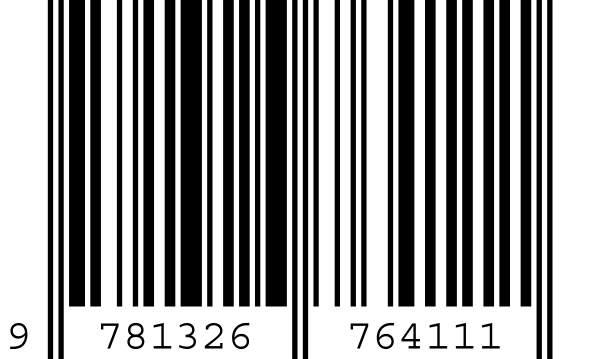
\includegraphics[width=4.7cm]{isbnbarcode}$
        	\end{minipage}
    	}
	}
}



\end{document}
